\documentclass[smallextended]{svjour3}
\smartqed

\usepackage[utf8]{inputenc}
\usepackage[T1]{fontenc}
\usepackage[numbers,sort&compress]{natbib}
\usepackage{amsmath,amssymb}
\usepackage{graphicx}
\usepackage{booktabs}
\usepackage{xcolor}
\definecolor{darkgreen}{HTML}{008000}
\usepackage{tikz}
\usetikzlibrary{arrows.meta,positioning,fit,backgrounds}
\usepackage{enumitem}
\usepackage{microtype}
\usepackage{placeins} % [section] RETIRÉ : Empêche la génération de trous blancs massifs
\usepackage[hidelinks,colorlinks=true,linkcolor=blue,citecolor=blue,urlcolor=blue]{hyperref}

\graphicspath{{figures/}}

\spnewtheorem{assumption}{Assumption}{\bfseries}{\rmfamily}
\spnewtheorem{empresult}{Empirical Result}{\bfseries}{\rmfamily}

% ── Stream S6 measured constants. Source: results/S6_synchronized_traces/.
% Every value is read from a committed artifact; none is typed by hand.
\newcommand{\SixSeeds}{100}                  % config/experiment_ssot.py S6_CAMPAIGN_SEEDS
\newcommand{\SixHorizon}{2500}               % S6_T_HORIZON
\newcommand{\DeltaPtext}{0.01}               % R2_CUSUM_DELTA = S6_AUDIT_DELTA_P
\newcommand{\SixCanonDeltaE}{0.3268}         % canonical grid point (transfer\_S1 label 0.33)
\newcommand{\SixTauFirst}{57.4}              % mean tau\_swap^(1/M), s6\_causal.json
\newcommand{\SixTauErase}{612}               % mean argmax A\_unrefl, s6\_causal.json
\newcommand{\SixMuWfirst}{18.2}              % (Delta e - delta\_P) * SixTauFirst
\newcommand{\SixMuWerase}{194}               % (Delta e - delta\_P) * SixTauErase
\newcommand{\SixCeilingFull}{31.3}           % median S\_max, arm full, canonical point
\newcommand{\SixCeilingNoSwap}{41.1}         % median S\_max, arm no\_swap
\newcommand{\SixCeilingFrozen}{650}          % median S\_max, arm frozen
\newcommand{\FullSpreadGrid}{6.58}           % max/min median S\_max, full, 20-point grid
\newcommand{\FrozenSpreadGrid}{133}          % idem, frozen (132.98)
\newcommand{\SuppressLo}{12}                 % frozen/full median ratio at Delta e = 0.24
\newcommand{\SuppressHi}{59}                 % idem at Delta e = 0.50
\newcommand{\StarvFullK}{1}                  % crossings of lambda=50, full, envelope
\newcommand{\StarvFullN}{1600}               % seed-runs, 16 magnitudes x 100 seeds
\newcommand{\StarvFullUpper}{0.35}           % Clopper-Pearson 95\% upper, percent
\newcommand{\StarvFrozenLower}{99.4}         % Clopper-Pearson 95\% lower, percent
\newcommand{\NoSwapLeak}{18}                 % percent detection at lambda=50, no\_swap, canonical
\newcommand{\SwapRatio}{17.9}                % tau\_swap^(1)/tau\_swap^(1/M), pooled median
\newcommand{\SwapElasticity}{0.66}           % AFT beta\_1
\newcommand{\SwapElasticityZ}{-14.9}         % z against H0 = 1
\newcommand{\LambdaFA}{15}                   % R4\_PHT\_LAMBDA. FIXED operating threshold, NOT a
                                             % calibration: ProteuS carries an identically zero
                                             % pre-drift error, so no false-alarm budget selects
                                             % 15 or any other value. Cf. the footnote at
                                             % \ref{sec:crossover} and Section~\ref{sec:limitations}.
\newcommand{\LambdaOpNarrow}{21.93}          % envelope\_stats.json, lambda\_op\_bootstrap 0.20\_0.40
\newcommand{\LambdaOpNarrowCI}{[19.88,\,22.40]}
\newcommand{\WideEnvUnstable}{62.6}          % percent of replicates with lambda\_op below LambdaFA
\newcommand{\EnvLo}{0.20}\newcommand{\EnvHi}{0.40}
\newcommand{\DeFloorLo}{0.085}\newcommand{\DeFloorHi}{0.141}
\newcommand{\QlowFloorLo}{9.38}\newcommand{\QlowFloorHi}{18.32}
\newcommand{\DeCrit}{0.120}                  % measured Action 4: 0.1197, n=300
\newcommand{\DeCritCI}{[0.114, 0.127]}       % 95% bootstrap CI (10,000 draws)

% ── Stream S8, ab initio arms. Source: results/S8\_ab\_initio/data/s8\_causal.json,
% decomposition\_ab\_initio.a\_pos\_common. Reference arm forked at tau*, not at the first swap.
% Every value is read from a committed artifact; none is typed by hand.
\newcommand{\LearnSharePure}{98.6}           % E\_learn\_pure / E\_total, learning with no tree
                                             % EVER replaced. 0.98637, n = 1999
\newcommand{\LearnSharePureCI}{[98.5,\,98.8]}% seed-paired bootstrap, 10\,000 resamples
\newcommand{\SwapFirstShare}{0.71}           % E\_swap\_first / E\_total, the FIRST replacement alone
\newcommand{\SwapFirstShareCI}{[0.63,\,0.78]}
\newcommand{\SwapRestShare}{0.56}            % E\_swap\_rest / E\_total, every later replacement
\newcommand{\SwapRestShareCI}{[0.47,\,0.67]}
\newcommand{\AbInitDetect}{49}               % detections out of 100 at lambda = 50, Delta\_e = 0.3268,
                                             % replacement suppressed from tau* onward (18 when
                                             % suppressed only after the first, 0 nominal)

% ── v4 abstract, stream S11-b. Source: results/S2\_theory/tables/s2\_gate\_T20.json and
% results/S2bis\_calibration/tables/s2bis\_proteus\_gate.json. Every value is read from a committed
% artifact; none is typed by hand.
\newcommand{\CeilingCanon}{33.5}             % budget\_restitution.measured.per\_magnitude at Delta e = 0.326793: 33.5115
\newcommand{\CeilingGridMin}{19.2}           % idem .min = 19.243
\newcommand{\CeilingGridMax}{36.6}           % idem .max = 36.6025, argmax at Delta e = 0.193621
\newcommand{\RcusumFifty}{59.3}              % floor\_and\_family.family\_requirements.common\_alpha\_ladder[3].R\_CUSUM = 59.2724
\newcommand{\RcusumOp}{31.2}                 % family\_requirements\_at\_lambda\_eq, couple S6 measured lambda\_op (c=0): 31.2007

% ── Stream S2 recomputation at the MEASURED base rate. Source: results/S2_theory/tables/.
% Every value is read from a committed artifact; none is typed by hand.
\newcommand{\PzeroMeas}{0.024}               % ssot.P0\_MEASURED; median e\_pre, arm full, n = 2000
\newcommand{\PzeroBand}{[0.015,\,0.032]}     % central 95 \% of per-run e\_pre, s2\_gate\_T20.json
\newcommand{\ThetaStar}{0.6813}              % Cramer root at PzeroMeas, delta\_P = DeltaPtext
\newcommand{\ArlFifteen}{4.0\times10^{6}}    % ARL\_0(lambda = 15), s2\_arl0\_columns.csv
\newcommand{\ArlFifty}{9.1\times10^{16}}     % ARL\_0(lambda = 50), idem
\newcommand{\FloorBand}{[13.9,\,18.3]}       % eq:floor\_chord over PzeroBand, s2\_gate\_T20.json
\newcommand{\ChiLoose}{6.74}                 % chi\^{}2 looseness factor at PzeroMeas
\newcommand{\FloodLamArf}{20.97}             % mean lambda\_calibrated, pht\_arf\_c1
\newcommand{\FloodLamHt}{132.50}             % idem, pht\_ht (insects\_per\_episode.parquet)
\newcommand{\FloodPredArf}{210}              % re-arm model, s2\_flooding\_retrodiction.json
\newcommand{\FloodPredHt}{28}                % idem
\newcommand{\FloodArlGap}{3\times10^{4}}     % shortfall factor of the ARL\_0 model

% ── Stream S2-bis, equal-false-alarm-budget calibration. Source: results/S2bis\_calibration/.
% Every value is read from a committed artifact; none is typed by hand.
\newcommand{\SpanOverWarm}{4.8}              % armed pre-change span / warm-up, gradual\_balanced
\newcommand{\LamEqArf}{93}                   % lambda\_eq at the span budget, PHT+ARF(c=1)
\newcommand{\LamEqHt}{186}                   % idem, PHT+HT
\newcommand{\FaSpanArf}{11.3}                % alarms over the span at the warm-up threshold, ARF
\newcommand{\FaSpanHt}{2.0}                  % idem, HT
\newcommand{\RhoRefMeas}{10.57}              % F1 ratio at the warm-up calibration (reproduced)
\newcommand{\RhoEqSpan}{1.27}                % F1 ratio at the span budget
\newcommand{\RhoEqSpanCI}{[1.16,\,1.43]}     % seed-paired bootstrap, 10\,000 resamples
\newcommand{\ThresholdShare}{90}             % \% of the log-ratio attributable to the threshold

% Artifact repository, anonymised. Declared once here so the venue never leaks into the body.
% \url{\RepoURL} expands only because this URL carries no catcode-active character. If it ever
% gains a # % ~ _ or &, switch the call site to \expandafter\url\expandafter{\RepoURL}.
\newcommand{\RepoURL}{https://anonymous.4open.science/r/TheBlindSpot-Experiments}

% ─────────────────────────────────────────────────────────────────
\journalname{Machine Learning}
\title{The Calibration Blind Spot: Sizing Cumulative Drift Monitors Against Adaptive Classifiers}
\titlerunning{The Calibration Blind Spot}
\authorrunning{Anonymous Author(s)}
\author{Anonymous Author(s)}
\institute{Anonymous Affiliation(s)}
\date{Received: date / Accepted: date}
% ─────────────────────────────────────────────────────────────────

\begin{document}
\maketitle

% ══════════════════════════════════════════════════════════════════
% ABSTRACT
% ══════════════════════════════════════════════════════════════════
\begin{abstract}
  Concept-drift monitoring composes an adaptive classifier with an external detector that reads
  the classifier's error stream. The composition closes a loop: the classifier reacts to the very
  residual the detector measures, so a persistent change leaves a transient signature and the
  evidence available to the monitor is bounded by adaptation rather than by the horizon. We treat
  the pipeline as fault detection on an endogenous residual and size it with two quantities in one
  unit---the evidence an adaptation leaves inside the window, and the evidence a monitor requires
  at a stated false-alarm level---so that a missed detection is attributed to a calibration rather
  than to a detector family. Synchronised instrumentation of $8{,}000$ runs measures the first
  directly: at the canonical operating point the median evidence ceiling is $\CeilingCanon$ (grid range
  $\CeilingGridMin$--$\CeilingGridMax$), which clears the information-theoretic floor $\FloorBand$ that binds every
  monitor of that false-alarm level. A cumulative monitor nonetheless reports no detection there,
  and the arithmetic states why: at $\lambda = 50$ its requirement is $\RcusumFifty$, while at the
  threshold the same certificate returns, $\lambda_{\mathrm{op}} = \LambdaOpNarrow$
  $\LambdaOpNarrowCI$, the requirement is $\RcusumOp$ and the ceiling clears it. The published collapses
  are threshold facts. On heteroscedastic ARMA--GARCH streams the same Page--Hinkley monitor that
  detects $0$ of $1{,}080$ drifts at the deployed threshold detects $1{,}080$ of $1{,}080$ at
  $\lambda = 5$ with precision $1.000$; the three detector families the evaluation compares are
  read at false-alarm levels thirteen orders of magnitude apart; and counterfactual arms sharing
  one stream and one fork assign $\LearnSharePure\%$ of the erasure to ordinary incremental learning with
  no tree replaced rather than to any internal detector. The rule these measurements support is
  operational: set the threshold from the false-alarm budget of the span the monitor will run armed
  over, on the error stream of the classifier it will be paired with, and check that the resulting
  requirement lies below the measured evidence ceiling. Validation spans instrumented Bernoulli
  streams, ProteuS, and six real-world streams (BAF, INSECTS), on which the two regime-dependent
  faces of the calibration---recall collapse and precision collapse---are reported separately.
\keywords{Concept drift \and Adaptive blind spot \and ADWIN \and Page-Hinkley \and Adaptive Random Forest}
\end{abstract}

% ══════════════════════════════════════════════════════════════════
\section{Introduction}\label{sec:intro}
% ══════════════════════════════════════════════════════════════════

An adaptive stream classifier repairs itself; it does not report.
When an Adaptive Random Forest (ARF)~\cite{gomes_arf_2017} replaces a drifting
subtree, predictive loss returns towards its pre-drift level and nothing else
leaves the model: no change timestamp, no localisation, no record a downstream
system can act on. Deployment separates three objectives that the streaming
literature routinely merges.
\emph{(i) Adaptation} minimises predictive loss; the model is its own consumer.
\emph{(ii) Monitoring and diagnosis} establish whether the environment changed,
when, and where; the consumers are the engineers who must decide whether a shift
is benign seasonality or a broken upstream feature.
\emph{(iii) System alarm} notifies operators, downstream pipelines and auditors.
Objectives (ii) and (iii) survive a model that repairs itself perfectly, because
their consumers are not the model. Regulation states the separation directly:
Article~15(4) of the EU Artificial Intelligence Act~\cite{eu_ai_act_2024}
requires providers of high-risk systems that keep learning after deployment to
eliminate or mitigate the feedback loops that continued learning creates, and
Article~72 requires a documented post-market monitoring system collecting
performance evidence over the system's lifetime. United States banking
supervision requires ongoing monitoring of deployed models under independent
effective challenge~\cite{frb_sr26_2_2026}. A model that silently absorbs a
change satisfies none of this.

The architecture we study---a self-updating model observed by a monitor it does
not control---is the ordinary shape of production monitoring. Managed services
attach drift and model-quality jobs to a deployed endpoint on their own
schedule~\cite{gcp_vertex_monitoring, aws_model_monitor}; open-source libraries
run the same checks in pipelines and CI~\cite{evidently_lib}; NannyML names its
object of observation \emph{the monitored model} and estimates that model's
performance from predictions when labels arrive late or never~\cite{nannyml_pe}.
None of these stacks assumes a frozen model, and none couples the monitor to the
model's update path. River~\cite{montiel_river_2021} and MOA ship both halves and
compose them. We claim no census of deployments; we claim that the composition is
the default design pattern and that regulation now requires the monitoring half
to stay independent of the adaptation half.

Composing the two halves closes a loop. Let $\tau^{*}$ denote the change instant,
$e_t \in \{0,1\}$ the classifier's error indicator at time $t$, and $\Delta e$ the
error excess the change induces before any adaptation. The external monitor
observes $e_t$; the classifier reacts to that same $e_t$ by replacing trees. The
measured signal is endogenous. Fault detection under feedback has studied this
configuration for three decades: a controller that rejects a disturbance also
removes it from the residual, and a residual-based detector loses the evidence it
was calibrated on~\cite{chen_patton_1999, gertler_1998, isermann_2006}. ARF's
internal ADWIN detectors~\cite{bifet_adwin_2007} act as a high-gain,
event-triggered corrector on the error rate; the external cumulative monitor is
the residual test. The change is not undone---the environment has shifted and
stays shifted---the loop has removed its signature.

Adaptation therefore converts a persistent change into a transient one. Write
$\tau_{\mathrm{erase}}$ for the erasure time: the delay from $\tau^{*}$ until
ensemble error returns to within tolerance of its pre-drift level. Any monitor
reading $e_t$ has $\tau_{\mathrm{erase}}$ observations of the change, not the
horizon of the stream. Cumulative-evidence monitors of the CUSUM
family~\cite{page_1954, lorden_1971, moustakides_1986} require a fixed quantity of
evidence, accumulated at a rate set by $\Delta e$, before stopping; when the
window closes first, no alarm fires. Stated this way the effect is a power
deficit under window truncation, and the design problem is a sizing problem: fit
the evidence a monitor requires inside the window the classifier leaves open.
Sequential detection of transient signals~\cite{nikiforov_2012,
tartakovsky_2023_transient} supplies the matching criterion---worst-case
probability of missed detection over a window of finite length at a fixed
false-alarm rate---in place of the F1 scores that dominate drift-detector
benchmarks and that fold calibration and delay into one scalar comparable across
no two detectors.

We call \textbf{blind spot} the region of the design space where the window
closes before the required evidence arrives, and \textbf{starvation} the
mechanism that closes it. Two consequences follow on the same threshold.
Raising the monitor's threshold to control false alarms lengthens the required
accumulation and widens the blind spot; lowering it to fit inside
$\tau_{\mathrm{erase}}$ floods a heteroscedastic stream with alarms. Recall
collapse on stationary streams and precision collapse on non-stationary ones are
the two faces of one calibration, not two phenomena
(Fig.~\ref{fig:ontology}). Our real-data streams exhibit the precision face; the
recall face is established on controlled and semi-synthetic streams, and we
mark the distinction wherever results are reported.

% Ontology of the retained effects. The terminal node is the comparison of the evidence budget A
% against the monitor's own requirement R(D, eps, alpha); the blind spot splits at the universal
% detection floor into an information-theoretic regime and a calibration regime; the requirement
% is shown as a function of the false-alarm level, beside the negative feedback loop, the single
% lambda axis carrying starvation and flooding, and the P(X) monitor outside the loop. Nodes are
% placed on an explicit millimetre grid; no \ref crosses out of this file, so it compiles against
% the preamble alone.
% Requires in the preamble:
%   \usepackage{tikz}
%   \usetikzlibrary{arrows.meta,positioning,fit,backgrounds}
\begin{figure}[t]
\centering
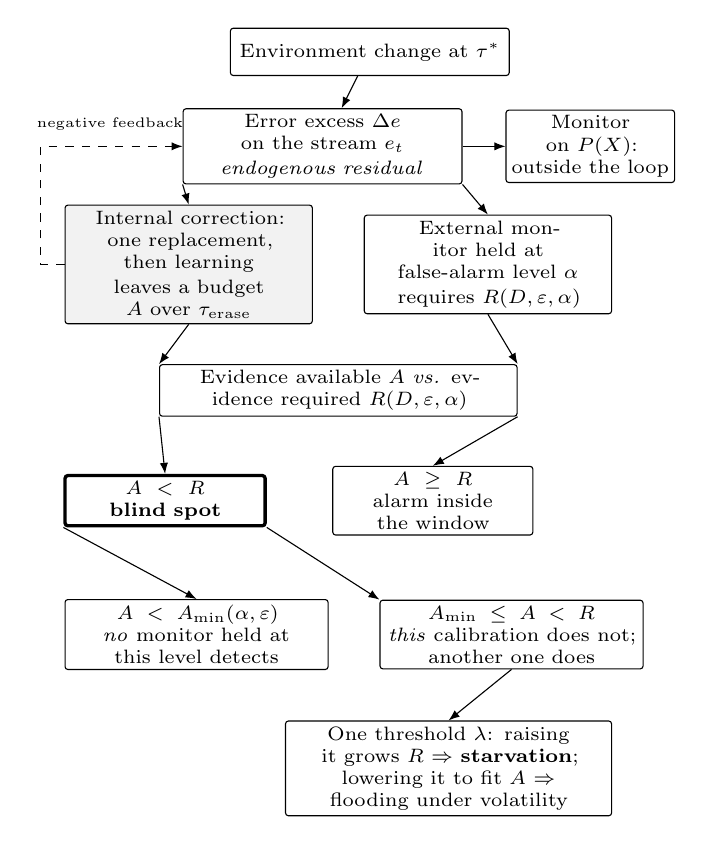
\begin{tikzpicture}[
  x=1mm, y=1mm,
  font=\scriptsize,
  box/.style   ={draw, rounded corners=1pt, align=center, inner sep=2pt,
                 text width=34mm, minimum height=6mm},
  loop/.style  ={box, fill=black!5},
  outcome/.style={box, text width=24mm},   % not `out`: /tikz/out is reserved by to[out=..]
  bad/.style   ={box, very thick, text width=24mm},
  ar/.style    ={-{Latex[length=1.4mm]}, thin},
  fb/.style    ={-{Latex[length=1.4mm]}, thin, dashed}
]

\node[box] (chg) at (0,0) {Environment change at $\tau^{*}$};
\node[box] (res) at (-6,-12)
  {Error excess $\Delta e$ on the stream $e_t$\\[1pt]\emph{endogenous residual}};
\node[outcome, text width=20mm] (px) at (28,-12)
  {Monitor on $P(X)$:\\outside the loop};

\node[loop, text width=30mm] (adapt) at (-23,-27)
  {Internal correction:\\one replacement, then learning\\[1pt]
   leaves a budget $A$ over $\tau_{\mathrm{erase}}$};
\node[box, text width=30mm] (mon) at (15,-27)
  {External monitor held at\\false-alarm level $\alpha$\\[1pt]
   requires $R(D,\varepsilon,\alpha)$};

\node[box, text width=44mm] (cmp) at (-4,-43)
  {Evidence available $A$ \emph{vs.} evidence required
   $R(D,\varepsilon,\alpha)$};

\node[bad] (blind) at (-26,-57) {$A < R$\\\textbf{blind spot}};
\node[outcome] (late) at (8,-57) {$A \geq R$\\alarm inside the window};

\node[outcome, text width=32mm] (info) at (-22,-74)
  {$A < A_{\min}(\alpha,\varepsilon)$\\\emph{no} monitor held at this
   level detects};
\node[outcome, text width=32mm] (cal) at (18,-74)
  {$A_{\min} \leq A < R$\\\emph{this} calibration does not;\\another one does};

\node[outcome, text width=40mm] (lam) at (10,-91)
  {One threshold $\lambda$: raising it grows $R$ $\Rightarrow$
   \textbf{starvation}; lowering it to fit $A$ $\Rightarrow$ flooding
   under volatility};

\draw[ar] (chg) -- (res);
\draw[ar] (res.south west) -- (adapt.north);
\draw[ar] (res.south east) -- (mon.north);
\draw[ar] (res.east) -- (px.west);
\draw[fb] (adapt.west) -- ++(-3,0) |- (res.west);
\node[font=\tiny, anchor=south] at (-33,-11.2) {negative feedback};
\draw[ar] (adapt.south) -- (cmp.north west);
\draw[ar] (mon.south)   -- (cmp.north east);
\draw[ar] (cmp.south west) -- (blind.north);
\draw[ar] (cmp.south east) -- (late.north);
\draw[ar] (blind.south west) -- (info.north);
\draw[ar] (blind.south east) -- (cal.north west);
\draw[ar] (cal.south) -- (lam.north);

\end{tikzpicture}
\caption{Relations between the retained effects. The classifier acts by negative
feedback on the very stream the monitor reads, so the evidence reaching the
monitor is a budget $A$ bounded by adaptation rather than by the horizon. The
terminal comparison is $A$ against the evidence $R(D,\varepsilon,\alpha)$ the
monitor's own false-alarm level requires: a blind spot is a deficit between two
quantities in one unit, and it splits at the universal detection floor
$A_{\min}(\alpha,\varepsilon)$. Below the floor no monitor held at that level
detects; above it the deficit belongs to this calibration, and another threshold
or another family meets the same budget. Recall collapse and precision collapse
are two settings of one threshold $\lambda$, not two phenomena. A monitor on the
input distribution is not exposed to the loop, at the cost of blindness to a
change in $P(Y\mid X)$ at fixed $P(X)$.}
\label{fig:ontology}
\end{figure}


\noindent\textbf{Contributions.}
\begin{enumerate}[nosep, label=\textbf{(C\arabic*)}]
  \item \textbf{Monitoring under closed-loop adaptation.} We state the concept-drift monitoring
  problem as fault detection on an endogenous residual, give the mapping to the
  fault-detection-under-feedback setting, and derive the prediction that severity is governed by
  the comparison of the evidence the loop leaves against the evidence the monitor's calibration
  requires---not by River, by ARF, or by ADWIN, and not by any one internal detector
  (Section~\ref{sec:blindspot}).
  \item \textbf{A transient-detection analysis of the sizing problem.} We characterise the
  observability window adaptation induces, define the blind spot as a deficit of budget against
  requirement in a single unit, and derive a detection floor that binds every monitor at a given
  false-alarm level. The floor separates two regimes: below it no monitor detects, above it the
  deficit is a property of the calibration and a different setting escapes it
  (Section~\ref{sec:framework}).
  \item \textbf{Synchronised measurement of the budget.} We instrument tree replacement, ensemble
  error and the monitor's statistic on a shared clock across counterfactual arms that share one
  stream, one history and one fork; we measure the evidence ceiling directly rather than through a
  rectangular surrogate, and we report the dilation between the first replacement and erasure as a
  measurement rather than as a definitional assumption (Section~\ref{sec:experiments}).
  \item \textbf{An ordering of monitor families, indexed by the stream.} We compare cumulative,
  adaptive-window and fixed-window two-sample monitors on the error stream at their deployed
  levels and at a common false-alarm level, on two streams whose pre-change error rate $p_0$ is
  not zero. Equalising the level lowers the fixed-window two-sample monitor (KSWIN, $0.458 \to
  0.337$ of runs detected) and raises the adaptive-window one (ADWIN, $0.885 \to 0.926$, median
  delay $28 \to 15$ steps), both at zero pre-change alarms: the deployed comparison orders
  calibrations, not families. EDDM has no rank of its own---it never arms at $p_0 = 0$, is first
  at $p_0 = 0.024$ ($0.974$ detected, $0.020$ pre-change alarms) and last at $p_0 = 0.069$
  ($0.022$ detected, $0.930$)---so the ordering is a table with $p_0$ as a column
  (Table~\ref{tab:family_order}), not a ranking. A monitor on the input distribution does not
  enter it: on a change of $P(Y \mid X)$ at fixed $P(X)$ it does not see the drift
  (Section~\ref{sec:related} and Section~\ref{sec:discussion}).
\end{enumerate}

% ══════════════════════════════════════════════════════════════════
\section{Background and Related Work}\label{sec:related}
% ══════════════════════════════════════════════════════════════════

\subsection{Detection and adaptation, evaluated apart}
Concept drift detection has been surveyed for two
decades~\cite{gama_survey_2014, lu_concept_drift_2018, bayram_2022}, from
Klinkenberg and Joachims~\cite{klinkenberg_2000} onwards. The surveys frame the
detector as a module serving the classifier: the detector fires, the classifier
adapts. Evaluation follows the frame. Detector
benchmarks~\cite{goncalves_2014, lukats_2025} run on pre-generated bitstreams
with no classifier in the loop; work introducing adaptive ensembles such as
ARF~\cite{gomes_arf_2017} or SRP~\cite{gomes_srp_2019} reports predictive
accuracy. Deployed pipelines stack the two. Stirling et
al.~\cite{stirling_2018} studied the effect of the internal detector on a
Hoeffding Adaptive Tree~\cite{bifet_hat_2009} and measured classification
accuracy only. Read~\cite{read_2018} flagged destructive adaptation in
Hoeffding-tree ensembles as a classification inefficiency and argued for
detector-free continuous adaptation; read from the monitoring side, the same
mechanism removes the evidence an external monitor needs.

\subsection{Fault detection on an endogenous residual}
Monitoring a signal that a controller is actively regulating is the standard
setting of model-based fault detection and isolation~\cite{chen_patton_1999,
gertler_1998, isermann_2006, blanke_2006}. A residual generator compares
observed behaviour to nominal behaviour and a decision rule tests the residual
for a shift. Under feedback the residual is no longer a free measurement: the
controller compensates the fault and the residual returns towards zero while the
fault persists, so residual sensitivity falls and detectability degrades. The
effect is reported across process control and is not confined to linear
plants---adaptive controllers mask fault signatures that data-driven detectors
rely on. Two properties transfer to our setting. Detectability is a property of
the loop, not of the detector alone. Instrumenting a signal the loop does not
close over restores it.

The mapping is structural and we state its limits. The plant is the conditional
law $P_t(Y \mid X)$; the fault is the change at $\tau^{*}$; the residual is the
error stream $e_t$; the controller is the internal drift-detection and
tree-replacement mechanism; the residual test is the external monitor. Unlike a
linear regulator with integral action, ARF's corrector is discrete,
event-triggered and non-parametric, so no transfer-function argument carries
over and we make none. What carries over is the topology and its consequence:
the quantity the monitor reads is a function of the corrector's own action.

\subsection{Change-point criteria}
Sequential change-point theory supplies the criteria we report against. Page's
CUSUM~\cite{page_1954} is minimax optimal for Lorden's worst-case expected
delay~\cite{lorden_1971, moustakides_1986}; Lai~\cite{lai_1995} unifies the
procedures scattered across quality control and fault detection; Tartakovsky,
Nikiforov and Basseville~\cite{tartakovsky_2014} give the reference treatment.
A detector is characterised by a pair: the in-control average run length
$\mathrm{ARL}_0$, and the detection delay attained at that $\mathrm{ARL}_0$. The
pair is comparable across detector families because it fixes calibration before
measuring speed. An F1 score computed over a matching window is not: it depends
on the window, on the number of true change points in the stream, and on an
implicit and unequal false-alarm budget per detector.

Changes of finite duration require a further departure. When a change persists
for a bounded interval, mean delay is the wrong functional and the criterion
becomes the worst-case probability of missed detection within the
interval~\cite{nikiforov_2012, tartakovsky_2023_transient}. Adaptation places our
problem in exactly this class: the interval is $\tau_{\mathrm{erase}}$, and it is
set by the classifier rather than by the environment.

\subsection{Monitoring deployed models}
Production monitoring separates the monitor from the model by
construction. Managed services schedule data-quality and model-quality jobs
against a deployed endpoint, comparing live features to a training
baseline and, where labels are ingested, live error to a baseline
error~\cite{gcp_vertex_monitoring, aws_model_monitor}. Open-source libraries run
equivalent checks offline and in pipelines~\cite{evidently_lib}. Where labels are
delayed, performance is estimated from prediction confidence or from a secondary
loss model~\cite{nannyml_pe}; both estimators assume the conditional law is
unchanged, so they degrade under precisely the drift they are deployed to
survive. None of these systems is coupled to the monitored model's own update
path, and Article~15(4) of the EU Artificial Intelligence
Act~\cite{eu_ai_act_2024} requires providers of continually learning high-risk
systems to address the feedback loops that continued learning creates.

\subsection{Monitors outside the loop}
A monitor that never reads $e_t$ is not exposed to erasure. Detectors on the
input distribution $P(X)$ compare a reference window to a current window:
Hellinger-distance monitoring on feature histograms~\cite{ditzler_hdddm_2011},
density comparison in a principal-component
subspace~\cite{qahtan_pcacd_2015}, and discriminative separability between the
two windows~\cite{gozuacik_d3_2019}. Margin-density
monitoring~\cite{sethi_md3_2017} sits between the families: it reads the
classifier's decision geometry rather than its realised error. Surveys and
benchmarks cover the family~\cite{gemaque_2020, hu_nofreelunch_2020,
lukats_2025}.

The exemption has a price, and it is symmetric. An input-space monitor is blind
to a change in $P(Y \mid X)$ at fixed $P(X)$---the case where the labelling rule
moves and the features do not---which is the case error-stream monitors are
built for. Neither family dominates. The design consequence is that the two
occupy different positions with respect to the loop and are therefore
complementary rather than substitutable. On the generators of this paper the
price is measured: a Hellinger-distance monitor~\cite{ditzler_hdddm_2011} that
detects a mean shift of the features ($0.35$, $0.55$ and $1.00$ of runs at
$0.25$, $0.5$ and $1$ standard deviation) returns the same output on every seed
at every drift magnitude, because both generators move the decision boundary at
fixed $P(X)$. It does not see the drift this paper studies.

\subsection{Detectors instantiated in this work}
\textbf{ADWIN}~\cite{bifet_adwin_2007} maintains a window split into two
sub-windows and declares a change when their means diverge beyond a Hoeffding
bound~\cite{hoeffding_1963}, testing every $c$ steps.
\textbf{PHT}~\cite{page_1954, basseville_1993} accumulates a running statistic
net of a tolerance $\delta_P>0$ and fires when it exceeds a threshold $\lambda>0$
governing $\mathrm{ARL}_0$. \textbf{DDM}~\cite{gama_ddm_2004} and \textbf{ECDD}~\cite{ross_ecdd_2012}
accumulate evidence on the error rate and are exposed to the same window
truncation. \textbf{EDDM}~\cite{baena_eddm_2006} is not: it compares the
cumulative mean and standard deviation of the distance between errors with their
running maximum, so the post-change evidence it needs grows with the stationary
history, and Section~\ref{sec:requirement} assigns it no requirement.
\textbf{KSWIN}~\cite{raab_kswin_2020} runs a two-sample test between a
reference reservoir and a recent window at a stated level $\alpha$ ($0.005$ as
deployed here), so its evidence requirement is set by the window and by
$\alpha$ rather than by an accumulated sum; at the false-alarm level of a
$\lambda = 50$ CUSUM it exceeds the measured evidence ceiling
(Remark~\ref{rem:split_measured}).

\subsection{Classifiers instantiated in this work}\label{sec:adwin}
\textbf{Hoeffding Trees (HT)}~\cite{gama_survey_2014} are incremental decision trees, \emph{non-adaptive} once converged. \textbf{Adaptive Random Forests (ARF)}~\cite{gomes_arf_2017} maintain $M$ HTs, each paired with an internal ADWIN: upon an internal drift warning the ARF pre-trains a background tree and, upon confirmation, instantly replaces the active tree. This adaptive \emph{tree-swap} mechanism is central to the blind spot phenomenon. Every ADWIN instance, internal or external, evaluates its test only every $c$ steps (Remark~\ref{rem:clock}). For the PHT, by Wald's equation, the expected accumulation time after an abrupt mean shift $\Delta\mu$ is $\tau_{\mathrm{det}} = \lambda / (\Delta\mu - \delta_P) = \mathcal{O}(1/\Delta e)$, where $\Delta e$ denotes the effective error jump.

\begin{remark}[Clock parameter]\label{rem:clock}
  ADWIN in River~\cite{montiel_river_2021} evaluates its statistical test every $c$ steps ($c=32$ by default). By contrast, River's Page-Hinkley Test (PHT) evaluates at every step (no clock parameter).
\end{remark}

% docs/manuscript/sections/framework_v2.tex
% Unified formal framework: observability, stopping times, evidence budget, proof requirement.

\section{Formal Framework}\label{sec:framework}

\subsection{Stream, Labels, and Observability}\label{sec:observability}

We consider a stream of pairs $(x_t, y_t)_{t \ge 1}$ drawn from a joint law
$P_t$ that is stationary before an unknown change point $\tau^*$ and
stationary after it. A classifier $C$ emits $\hat{y}_t$ and the
\emph{prediction error} is $e_t := \mathbf{1}[\hat{y}_t \ne y_t]$.
Write $\bar{e}_t := \mathbb{E}[e_t]$ for its expectation under the joint law
of stream and classifier, $p_0 := \bar{e}_t$ for $t < \tau^*$ for the
pre-change error rate, and $\Delta e := \sup_{t \ge \tau^*} \bar{e}_t - p_0$
for the error jump.

\begin{assumption}[Observability split]\label{ass:obs}
  The change point $\tau^*$ and the post-change law $P_{\tau^*+}$ are
  unobservable. The error $e_t$ is observable exactly when $y_t$ is revealed.
\end{assumption}

Assumption~\ref{ass:obs} fixes the semantics of every subsequent statement:
what is hidden is the drift \emph{state}, never the error \emph{stream}.

\begin{definition}[Label protocol]\label{def:labels}
  A label protocol $\Pi$ reveals $y_t$ at time $t + \ell$ with probability
  $p \in (0,1]$, independently across $t$. Immediate supervision is
  $\Pi(\ell{=}0, p{=}1)$. The \emph{label clock} indexes the subsequence of
  revealed labels; the \emph{stream clock} indexes $t$.
\end{definition}

\begin{definition}[Monitor and windowed false-alarm level]\label{def:monitor}
  A monitor $D$ is a stopping time $\tau_{\mathrm{det}}$ adapted to the
  filtration generated by the observed errors. Its \emph{initial law} is
  part of the definition: the statistic is restarted at the change point,
  $S_{\tau^*} = 0$, and its reference level is the plug-in estimate
  $\hat p_0$ read from the $1000$ steps immediately before $\tau^*$ ---
  the construction every cumulative-evidence number in this paper is
  measured under. Its \emph{windowed false-alarm level} at horizon $W$ is
  $\alpha := \mathbb{P}_0(\tau_{\mathrm{det}} \le W)$, the probability of
  alarming within $W$ consecutive steps under the no-change law $P_0$.
\end{definition}

Definition~\ref{def:monitor} replaces family-specific tuning constants by a
single quantity shared by every sequential test. For the restarted
StrictCUSUM of Eq.~\eqref{eq:cusum} at increments
$+(1 - \hat p_0 - \delta_P)$ on an error and $-(\hat p_0 + \delta_P)$
otherwise, $\alpha$ is a first-passage probability from $0$ and is computed
\emph{exactly} by a lattice recursion under the i.i.d.\ Bernoulli($\hat p_0$)
null; the geometric approximation $\alpha \approx W/\mathrm{ARL}_0$ standard
in statistical process control is \emph{not} used, because it ignores the
dead time a restart at $\tau^*$ imposes: at
$(\hat p_0, \delta_P) = (0.024, 0.01)$ a threshold $\lambda = 50$ cannot be
reached in fewer than $52$ steps, and at the first-swap window of
$57.4$ steps the exact level is $2.2 \times 10^{-78}$ where the geometric
approximation returns $6.3 \times 10^{-16}$ --- sixty-two orders of
magnitude apart, on the quantity every floor of
Theorem~\ref{thm:floor} consumes through $\ln(1/\alpha)$. The reference
$\hat p_0$ is itself dispersed: over the campaign's $8{,}000$ runs the
$1000$-step estimate falls at or below $\hat p_0 - \delta_P$ in $1.75\%$ of
them, a case in which the null drift of the restarted statistic is
non-negative and no per-run Cram\'er root represents it; the exact levels
and floors below are therefore stated at the measured median
$\hat p_0 = 0.024$ and banded over its central $95\%$
(Remark~\ref{rem:floor_band}).

\begin{lemma}[Label-clock invariance]\label{lem:clock}
  If $C$ and $D$ consume the same label subsequence, then the quantities
  $A$ and $R$ of Definitions~\ref{def:budget} and~\ref{def:requirement} are
  invariant under $\Pi(\ell, p)$ when evaluated in the label clock.
\end{lemma}

\begin{proof}
  A uniform latency $\ell$ shifts both the adaptation and the detection
  filtrations by the same $\ell$, leaving every difference of stopping times
  unchanged. Under thinning at rate $p$, $C$ requires the same number of
  labelled examples to complete adaptation, so the recovery window dilates by
  $1/p$ in the stream clock, while the number of monitor updates inside that
  window contracts by $p$. The two factors cancel.
\end{proof}

Lemma~\ref{lem:clock} fails only when the monitor and the classifier read
different filtrations, e.g.\ an unsupervised feature-space monitor paired
with a supervised learner.

\subsection{Adaptation Times}\label{sec:times}

Let $M$ be the ensemble size and $N_{\mathrm{swap}}(t)$ the number of base
learners replaced in $(\tau^*, t]$.

\begin{definition}[Adaptation times]\label{def:times}
  For $q \in (0,1]$ and $\rho > 0$,
  \begin{align*}
    \tau_{\mathrm{swap}}^{(q)} &:= \inf\{\, t \ge \tau^* :
      N_{\mathrm{swap}}(t)/M \ge q \,\}, \\
    \tau_{\mathrm{err}}(\rho) &:= \inf\{\, t \ge \tau^* :
      \bar{e}_s \le p_0 + \rho \ \ \forall s \ge t \,\}, \\
    \tau_{\mathrm{erase}} &:= \tau_{\mathrm{err}}(\delta_P), \qquad
    W := \tau_{\mathrm{erase}} - \tau^*,
  \end{align*}
  where $\delta_P > 0$ is the drift tolerance of the monitor and $W$ is the
  \emph{exploitable transient}.
\end{definition}

\begin{proposition}[Ordering]\label{prop:order}
  $\rho \mapsto \tau_{\mathrm{err}}(\rho)$ is non-increasing and
  $q \mapsto \tau_{\mathrm{swap}}^{(q)}$ non-decreasing. If the ensemble error is
  not already within tolerance for every $s \ge t$ at some
  $t < \tau_{\mathrm{swap}}^{(1/M)}$ --- that is, if the drift is not resolved
  before the first replacement --- then
  $\tau_{\mathrm{swap}}^{(1/M)} \le \tau_{\mathrm{erase}}$.
\end{proposition}

\begin{proof}
  Monotonicity is immediate from Definition~\ref{def:times}: enlarging $\rho$
  weakens the constraint defining $\tau_{\mathrm{err}}(\rho)$, so its infimum
  cannot increase; raising $q$ strengthens the constraint defining
  $\tau_{\mathrm{swap}}^{(q)}$, so its infimum cannot decrease.

  For the inequality, write $t_1 := \tau_{\mathrm{swap}}^{(1/M)}$ and suppose
  $\tau_{\mathrm{erase}} < t_1$. By Definition~\ref{def:times},
  $\tau_{\mathrm{erase}} = \tau_{\mathrm{err}}(\delta_P)$ is the infimum of the
  times $t$ at which $\bar{e}_s \le p_0 + \delta_P$ holds \emph{for every}
  $s \ge t$. So $\tau_{\mathrm{erase}} < t_1$ exhibits a
  $t < t_1$ at which the error is already within tolerance for all subsequent
  $s$ --- which is exactly the hypothesis excluded. Hence
  $t_1 \le \tau_{\mathrm{erase}}$.

  The universal quantifier over $s \ge t$ is what carries the argument, and it is why the ordering does not need the pointwise assumption of Remark~\ref{rem:order}: a transient dip of $\bar{e}$ below $p_0 + \delta_P$
  at some $t < t_1$ does not make $t$ admissible unless the error stays there,
  so it cannot move $\tau_{\mathrm{err}}$. The hypothesis excluded above is
  strictly weaker than that assumption --- it forbids \emph{resolution} before
  the first replacement, not \emph{elevation} at every step before it --- and it
  is the weakest hypothesis under which the conclusion can hold, since its
  negation is the conclusion's negation. Measured status: the conclusion holds
  in $1{,}835$ of the $1{,}836$ runs where $\tau_{\mathrm{erase}}$ is
  estimable, and in all $2{,}000$ under the hysteresis estimator.
\end{proof}

\begin{remark}[The ordering is measured, not assumed]\label{rem:order} The inequality follows immediately from an assumption of \emph{no recovery without replacement}: $\bar{e}_t > p_0 + \delta_P$ pointwise on $[\tau^*, \tau_{\mathrm{swap}}^{(1/M)})$. That assumption is contradicted by measurement, and we do not use it. Synchronised instrumentation refutes
  it ($100$ seeds $\times$ $20$ magnitudes of the nominal arm, $\delta_P = 0.01$).
  Under a cumulative mean from $\tau^*$ it holds in $31.0\%$ of $2{,}000$ runs;
  under a $20$-step trailing mean, in $83.1\%$; and under the $200$-step window
  $\bar{e}_t$ actually denotes it is not evaluable at all on the $89.7\%$ of
  intervals shorter than the window itself, holding in $57.0\%$ of the remainder.
  The failure rate is monotone in magnitude and reaches no majority at any grid
  point.

  The ordering survives because it never needed that much. $\tau_{\mathrm{err}}$
  quantifies over \emph{all} $s \ge t$, so the transient dips that break the
  pointwise reading do not move it: $\tau_{\mathrm{erase}} \ge
  \tau_{\mathrm{swap}}^{(1/M)}$ in $1{,}835$ of the $1{,}836$ runs where
  $\tau_{\mathrm{erase}}$ is estimable, and in all $2{,}000$ under the hysteresis
  estimator. The assumption was strictly stronger than the conclusion it was
  introduced to support, and false exactly where it exceeded it.

  The converse bound $\tau_{\mathrm{erase}} \le \tau_{\mathrm{swap}}^{(1)}$ does not follow from that assumption either, and fails on its own evidence: it holds in $55.3\%$ of the runs where both sides
  are defined, and $\tau_{\mathrm{swap}}^{(1)}$ is itself undefined in $11.3\%$ of
  runs, the sweep of all $M$ trees never completing within the horizon. Audit:
  \path{experiments/S6_synchronized_traces/s6_audit_ass_repair.py}.
\end{remark}

\begin{definition}[Dilation ratio]\label{def:kappa}
  $\kappa := (\tau_{\mathrm{erase}} - \tau^*) /
             (\tau_{\mathrm{swap}}^{(1/M)} - \tau^*)$.
\end{definition}

The first swap is retained as an instrumented lower bound on $W$; $\kappa$ is measured, never assumed: asserting $\kappa \ge 1$ inside the definition would make a claim about measured quantities under the guise of a definition.
Measured, $\kappa \ge 1$ in $1{,}835/1{,}836$ runs, median $14.6$; the single
exception is a run whose $200$-step trailing mean reports erasure before the first
replacement, a lag artefact of the estimator rather than a recovery.
$\kappa \ge 1$ is exactly the conclusion of Proposition~\ref{prop:order} divided
by $\tau_{\mathrm{swap}}^{(1/M)} - \tau^* > 0$, so it inherits that
proposition's hypothesis and nothing more: it holds whenever the drift is not
resolved before the first replacement, and it is not an assumption of
Definition~\ref{def:kappa}. Definition~\ref{def:kappa} requires only
$\tau_{\mathrm{swap}}^{(1/M)} > \tau^*$, which the campaign satisfies on
$2{,}000$ of $2{,}000$ cells.

\subsection{Proof Budget}\label{sec:budget}

\begin{definition}[Proof budget]\label{def:budget}
  \begin{equation}\label{eq:budget}
    A \;:=\; \sum_{t = \tau^*+1}^{\tau_{\mathrm{erase}}}
             \bigl(\bar{e}_t - p_0 - \delta_P\bigr)^{+} .
  \end{equation}
\end{definition}

$A$ is the integrated excess error above the monitor's tolerance over the
exploitable transient, measured in units of excess errors. It depends on the
classifier and the stream, never on the monitor beyond the scalar
$\delta_P$. A rectangular transient of height $\Delta e$ and duration $W$
gives $A = (\Delta e - \delta_P)\,W$.

\begin{proposition}[Budget invariance]\label{prop:invariance}
  Assume (i) a \emph{rectangular} transient, $A = (\Delta e - \delta_P) W$, and
  (ii) an adaptation time obeying the power law
  $W(\Delta e) = K (\Delta e)^{-\alpha}$. Then
  \begin{equation}\label{eq:invariance}
    A \;=\; K (\Delta e)^{1-\alpha}\bigl(1 - \delta_P/\Delta e\bigr),
  \end{equation}
  so at $\alpha = 1$ exactly, $A = K(1 - \delta_P/\Delta e) \to K$ as
  $\Delta e / \delta_P \to \infty$: the proof budget is asymptotically
  independent of the drift magnitude. For $\alpha \ne 1$ the budget is not
  constant but varies as $(\Delta e)^{1-\alpha}$.
  Proof: Appendix~\ref{sec:prop3}.
\end{proposition}

Proposition~\ref{prop:invariance} is the formal content of the magnitude invariance.
Increasing the magnitude of a drift does not increase the evidence delivered
to an external monitor, because adaptation accelerates in proportion.

\begin{remark}[Both hypotheses are measured, and both are contradicted]\label{rem:invariance_measured}
  Hypothesis~(i) is the rectangular surrogate that synchronised instrumentation
  withdraws: $A/A_{\mathrm{rect}}$ spans $2.70$ to $-14.12$ over the magnitude
  grid and \emph{changes sign} at $\Delta e \ge 0.452$, where the adapted
  ensemble ends the window below its pre-change error rate. That sign change is
  a property of the \emph{generator} and is reported as such: the boundary-shift
  family carries a post-drift class prior $P(y{=}1) = 0.5 - \Delta e$, which
  falls under $2.5\%$ over the last seven magnitudes, so the drift makes the
  problem easier and the integrated excess turns negative. On a rotation family
  with the same $\Delta e$ but a class balance held at $50/50$ --- the post-drift
  half-plane turned by $\theta = \pi \Delta e / (1 - 2\eta)$, label noise $\eta$
  giving a Bayes error that does not vanish --- the same ratio is monotone
  increasing to $+8.0$ at the top magnitude and negative on no run, against
  $100\%$ of runs negative on the boundary-shift family. The withdrawal of
  hypothesis~(i) does not depend on the generator; the sign change does. Hypothesis~(ii) is
  measured at $\hat\alpha \approx 0.98$, not $1$; by~\eqref{eq:invariance} that
  predicts a spread of $(0.50/0.10)^{0.02} = 1.03$ over the envelope. The
  measured threshold-free ceiling --- the peak $S_{\max}$ of the reflected
  walk of Eq.~\eqref{eq:cusum} at the declared tolerance $\delta_P = 0.01$,
  the statistic every ceiling in this paper is quoted on --- spreads by a
  factor $1.76$ ($19.1$ to $33.6$) and is \emph{non-monotone}, peaking near
  $\Delta e \approx 0.19$; the claimed band $A \in [16.8, 18.1]$ with $K = 18.5$
  is exceeded at every magnitude of the envelope.

  What survives is the comparative statement, and it survives on a
  counterfactual rather than on a power law: on the \texttt{no\_swap} and
  \texttt{frozen} branches of the same streams, where adaptation is suppressed,
  the same ceiling spreads by a factor of $133$ and is monotone increasing.
  Invariance is therefore an \emph{effect of adaptation}, demonstrated by
  removing it, and not a consequence of an exponent equal to one.
\end{remark}

\begin{empresult}[The evidence bell over the magnitude grid]\label{res:bell}
  The peak of the reflected walk of Eq.~\eqref{eq:cusum} over the post-drift
  horizon, $\mathbb{E}[S_{\max}(H)]$ (nominal arm, $H = 2000$,
  $\delta_P = 0.01$, $100$ seeds per amplitude), is unimodal over the
  magnitude grid: it rises from $5.28$ $[5.01, 5.55]$ at $\Delta e = 0.028$
  to a plateau near $33$ over $\Delta e \in [0.19, 0.25]$, then falls
  monotonically to $19.13$ $[18.73, 19.50]$ at $\Delta e = 0.498$. The two
  plateau points differ by $0.58$ against bootstrap half-widths of $0.97$,
  so the mode is not separable at $100$ seeds per amplitude and we report
  the plateau rather than a point. Past the plateau a stronger drift
  delivers \emph{less} evidence --- the reflected counterpart of the
  unreflected ceiling of Remark~\ref{rem:invariance_measured} --- because
  adaptation consumes the transient faster than the walk accumulates it.
\end{empresult}

\begin{empresult}[The trivial floor at the degenerate end]\label{res:skillfloor}
  The highest grid points carry a minority prior below $1.8\%$, and there
  the adaptive ensemble stops beating the constant majority-class
  predictor. The skill score is reported against two error estimators,
  because they answer different questions and disagree on how far the
  deficit extends. Against the mean error over the post-drift episode ---
  which charges the ensemble for a transient the constant predictor never
  pays --- skill turns negative from $\Delta e = 0.482$ and reaches $-3.47$
  at $\Delta e = 0.498$. Against the converged residual error (mean over
  the last $200$ steps of the horizon), which no transient can explain
  away, skill stays non-negative over the grid but collapses onto the
  trivial floor at the last three magnitudes: $+0.06$ $[-0.13, +0.23]$,
  $+0.01$ $[-0.22, +0.23]$ and $+0.02$ $[-0.26, +0.29]$, every interval
  straddling zero. These intervals carry few events: at $\Delta e = 0.498$
  the trivial floor is $0.23\%$, so the last $200$ steps of $100$ runs
  contain $46$ errors in total ($105$, $72$ and $46$ across the three
  magnitudes). Every interval is therefore reported with its event count,
  and the comparison is widened to the last $1000$ steps of the horizon ---
  the transient is over within $\sim 30$ steps at these magnitudes, so the
  widened window charges no transient --- where the same amplitudes carry
  $501$, $340$ and $212$ errors: $+0.10$ $[+0.02, +0.18]$, $+0.07$
  $[-0.04, +0.17]$ and $+0.09$ $[-0.03, +0.21]$. Widened, the window
  resolves a small positive advantage at $\Delta e = 0.494$; the two most
  degenerate magnitudes remain statistically indistinguishable from the
  trivial floor, and there the equality is a result, not a limit of the
  window. Under either reading the right end of the grid describes
  a degenerate classification problem rather than a monitoring one, and
  every residual error there is reported with its trivial floor beside it.
\end{empresult}

\begin{remark}[The first replacement, isolated]\label{rem:first_swap}
  The two counterfactual arms of the synchronised campaign fork \emph{at}
  $\tau_{\mathrm{swap}}^{(1/M)}$ and therefore share the first replacement with
  the nominal arm; no contrast among them can attribute anything to it. Two
  further arms fork at $\tau^*$ instead --- an instant fixed by the protocol
  rather than by the trajectory --- with both internal detector paths made
  inert, the second additionally stopping \texttt{learn\_one}. With the
  $\tau^*$-frozen arm as the single reference the decomposition closes
  identically,
  \[
    E_{\mathrm{total}} = E_{\mathrm{learn}} + E_{\mathrm{swap}}^{(1)}
                       + E_{\mathrm{swap}}^{(>1)} ,
  \]
  measured additivity residual $2.3\times10^{-13}$ over $1{,}999$ cells. Over
  $100$ seeds and $20$ magnitudes, incremental learning with \emph{no} tree ever
  replaced accounts for $98.64\%$ of the erasure ($95\%$ seed-paired bootstrap
  $[98.48, 98.82]$), the first replacement alone for $0.71\%$
  $[0.63, 0.78]$, and every later replacement together for $0.56\%$
  $[0.47, 0.67]$. The first replacement therefore carries \emph{more} of the
  erasure than all its successors combined.

  The volumetric share understates it at the threshold. At $\Delta e = 0.3268$
  and $\lambda = 50$ the external CUSUM fires in $0$ of $100$ nominal runs, $18$
  of $100$ when replacement is suppressed after the first, and $49$ of $100$
  when it is suppressed from $\tau^*$ onward. Isolating the first replacement is
  worth $31$ points of detection rate --- more than suppressing every
  replacement after it.
\end{remark}

\subsection{Proof Requirement}\label{sec:requirement}

\begin{definition}[Proof requirement]\label{def:requirement}
  For a monitor $D$, a miss level $\varepsilon \in (0,1)$ and a windowed
  false-alarm level $\alpha$,
  \[
    R(D, \varepsilon, \alpha) := \inf\bigl\{\, a > 0 :
      A \ge a \Rightarrow
      \mathbb{P}(\tau_{\mathrm{det}} \le \tau^* + W) \ge 1 - \varepsilon
      \,\bigr\},
  \]
  the infimum being taken over error trajectories of window $W$ compatible
  with budget $A$.
\end{definition}

\begin{definition}[Blind spot]\label{def:blindspot}
  A pipeline $(C, D)$ exhibits a \emph{blind spot} at $(\Delta e, W)$ when
  $A < R(D, \varepsilon, \alpha)$.
\end{definition}

\begin{remark}[Scope of the predicate]\label{rem:predicate_scope}
  The budget $A$ of Definition~\ref{def:blindspot} is the evidence a monitor
  spends when its window can span the whole transient, as for the cumulative
  statistics and ADWIN. A fixed-window two-sample monitor reads at most
  $\min(W, n_{\mathrm{stat}})$ steps of the transient at once, so the budget is
  not the quantity its detection tracks: its condition is the contrast
  of~\eqref{eq:Rkswin_contrast}, a mean-field boundary whose scope
  Remark~\ref{rem:window_requirement} measures. We state the two conditions
  separately; a single predicate covering both was pre-registered and not
  retained (Section~\ref{sec:limitations}).
\end{remark}

Definition~\ref{def:blindspot} compares two quantities in the same unit and
contains no implementation constant. It supersedes any condition coupling an
ADWIN clock to a CUSUM threshold.

\begin{empresult}[The budget is the sufficient statistic; the erasure time is
not]\label{res:budget_sufficient}
  Nine pipelines --- an ARF driven by each of ADWIN, DDM, EDDM, PageHinkley and
  KSWIN, plus SRP, leveraging bagging, ADWIN bagging and a Hoeffding adaptive
  tree --- were run over six magnitudes with the external monitor calibrated to
  one false alarm per warm-up \emph{per pipeline}. Grouped by $A$, the miss-rate
  curves collapse: in the single budget band whose outcome is not saturated at
  $0$ or $1$, the miss rate is monotone in the band's median $A$ across every
  mechanism present. Grouped by $\tau_{\mathrm{erase}}$ they do not. At
  $\Delta e = 0.327$ the DDM-driven forest erases over $836$ steps against the
  ADWIN-driven forest's $808$ --- within $3.4\%$ --- and leaves $A = 75.4$
  against $43.9$; at $\lambda = 50$ the first is never missed in $30$ runs and
  the second is missed in $77\%$ of $30$. Erasing over the same window does not
  mean leaving the same evidence, and only the second decides.
\end{empresult}

The blind spot is therefore a statement about the budget, not about the
mechanism and not about the erasure time. The internal detector enters only
through the $A$ it leaves, which is what makes
Definition~\ref{def:blindspot} implementation-free rather than merely
implementation-agnostic.

\begin{theorem}[Universal detection floor]\label{thm:floor}
  Write $\pi_t := \mathbb{P}_1(e_t = 1 \mid \mathcal{F}_{t-1})$ for the
  conditional error probability under the post-change law, given the
  observed past, and assume, on the window $(\tau^*, \tau^* + W]$:
  \emph{(i)} the no-change law of the observed errors is i.i.d.\
  Bernoulli($p_0$), so the conditional null rate is $p_0$ after every
  past; \emph{(ii)} $\pi_t - p_0 \in [0, \Delta_{\max}]$ almost surely.
  Let $\Delta_{\max}$ be any almost-sure bound so defined. Every monitor
  satisfying Definition~\ref{def:monitor} at level $\alpha$ and detecting
  with probability at least $1 - \varepsilon$ within $W$ obeys
  \begin{equation}\label{eq:floor}
    A \;\ge\; \frac{p_0(1-p_0)}{\Delta_{\max}}\,
              d\bigl(1-\varepsilon \,\Vert\, \alpha\bigr) \;-\; W \delta_P ,
  \end{equation}
  where $d(a \Vert b) := a \ln(a/b) + (1-a)\ln\frac{1-a}{1-b}$ is the binary
  Kullback--Leibler divergence.
\end{theorem}

\begin{proof}
  Let $P_1$ be the post-change law and $P_0$ the no-change law restricted to
  the $W$ error observations. By the chain rule,
  $\mathrm{KL}(P_1 \Vert P_0) = \sum_t \mathbb{E}_1\bigl[
  d(\pi_t \Vert \pi_t^{(0)})\bigr]$, the expectation being over the
  filtration generated by the past; hypothesis~(i) makes
  $\pi_t^{(0)} = p_0$ after every past, so each term is
  $d(\pi_t \Vert p_0)$. Hypothesis~(ii) confines $\pi_t - p_0$ to
  $[0, \Delta_{\max}]$, where $u \mapsto d(p_0 + u \Vert p_0)$ is convex and
  vanishes at $u = 0$, so $d(\pi_t \Vert p_0) \le
  \bigl((\pi_t - p_0)/\Delta_{\max}\bigr)\, d_{\max}$ with
  $d_{\max} := d(p_0 + \Delta_{\max} \Vert p_0)$; the product form of the
  marginal rates is a lower bound on this conditional sum and is not used.
  Taking expectations and writing $u_t := \mathbb{E}_1[\pi_t] - p_0$ gives
  $\mathrm{KL}(P_1 \Vert P_0) \le (d_{\max}/\Delta_{\max}) \sum_t u_t$.
  Since $u_t \le (u_t - \delta_P)^{+} + \delta_P$,
  $\sum_t u_t \le A + W\delta_P$, and $d_{\max} \le
  \Delta_{\max}^2/(p_0(1-p_0))$ (the $\chi^2$ bound applied once) gives
  $\mathrm{KL}(P_1 \Vert P_0) \le \Delta_{\max}(A + W\delta_P) /
  (p_0(1-p_0))$. Applying the data-processing inequality to the event
  $E := \{\tau_{\mathrm{det}} \le \tau^*+W\}$, which has $P_1$-probability at
  least $1-\varepsilon$ and $P_0$-probability at most $\alpha$, yields
  $\mathrm{KL}(P_1 \Vert P_0) \ge d(1-\varepsilon \Vert \alpha)$.
  Rearranging gives~\eqref{eq:floor}.
\end{proof}

Both hypotheses are stated, not tacit. Hypothesis~(i) is the idealised null:
the measured pre-change error rate is itself dispersed
(Remark~\ref{rem:floor_band}), and the floors are banded over that
dispersion. Hypothesis~(ii) has a measured upper end and an idealised lower
one. The upper end is measured on the arm frozen at $\tau^*$, whose model
never updates after the change, so its error rate \emph{is} the conditional
probability $\pi$ under the post-change law: over the $100$ runs at
$\Delta e = 0.3268$ the per-run estimate (2500 steps) has median $0.332$ and
maximum $0.358$ absolute, $0.333$ in excess of its own pre-change rate, and
we charge every floor at $\Delta_{\max} = 0.36$, which covers that maximum
plus three standard errors ($0.009$) of the estimate. The lower end
($\pi_t \ge p_0$: no adaptation below baseline inside the window) is
measured false at the canonical point over the full horizon --- the
$200$-step trailing error rate dips below the pre-change rate in $100$ of
$100$ runs, by a median $0.022$ --- so the floor is a statement about the
window in which the transient lives, not about the adapted tail that
follows it.

Theorem~\ref{thm:floor} separates two regimes. When $A$ falls below the
right-hand side of~\eqref{eq:floor}, no monitor of that false-alarm level
detects, and the blind spot is information-theoretic. When $A$ exceeds it
while remaining below $R(D,\varepsilon,\alpha)$, the blind spot is a property
of $D$'s calibration, and a different monitor family escapes it.

\begin{remark}[The $\chi^2$ step is where~\eqref{eq:floor} loses its strength]\label{rem:floor_tight}
  The proof relaxes each chain-rule term by $d(x \Vert y) \le (x-y)^2/(y(1-y))$,
  which is the $\chi^2$ bound. Since $u \mapsto d(p_0 + u \Vert p_0)$ is convex
  on $[0, \Delta_{\max}]$ and vanishes at $u = 0$, the chord through the
  endpoints gives directly
  $d(p_0+u \Vert p_0) \le (u/\Delta_{\max})\, d_{\max}$ with
  $d_{\max} := d(p_0 + \Delta_{\max} \Vert p_0)$, hence the strictly stronger
  \begin{equation}\label{eq:floor_chord}
    A \;\ge\; \frac{\Delta_{\max}}{d_{\max}}\, d(1-\varepsilon \Vert \alpha)
              \;-\; W \delta_P .
  \end{equation}
  The two coincide only as $\Delta_{\max}/p_0 \to 0$. At the measured
  $p_0 = 0.024$ and the measured almost-sure bound
  $\Delta_{\max} = 0.36$ the $\chi^2$ step costs a
  factor $7.08$, so~\eqref{eq:floor} understates the floor by nearly an order
  of magnitude precisely at the operating point the experiments occupy. All
  floors quoted below use~\eqref{eq:floor_chord}.
\end{remark}

\begin{remark}[The floor is evaluated at the exact level, and banded over the
measured reference]\label{rem:floor_band}
  $\hat p_0$ is not a determined quantity on these streams. The pre-change
  error rate is measured per run, and over the central $95\%$ of its empirical
  distribution, $p_0 \in [0.015, 0.032]$, the Cram\'er root moves from $0.968$
  to $0.542$ and $\mathrm{ARL}_0$ at $\lambda = 50$ spans $1.1\times10^{14}$
  to $1.1\times10^{23}$ --- nine orders of magnitude. No scalar evaluation of
  any quantity consuming $\mathrm{ARL}_0$ is reportable at that dispersion,
  and none is attempted: the level $\alpha$ that the floor consumes is the
  \emph{exact} first-passage probability of the restarted statistic
  (Definition~\ref{def:monitor}), recomputed at each point of the band, so
  $\mathrm{ARL}_0$ enters no published floor at all.

  Over the same band, \eqref{eq:floor_chord} at $\Delta e = 0.3268$,
  $\Delta_{\max} = 0.36$, $\lambda = 50$ and the first-swap window
  $\tau_{\mathrm{swap}}^{(1/M)} = 57.4$ in place of $W$ evaluates to
  $[74.7,\, 82.3]$ --- a $\pm 5\%$ interval around its midpoint. Every
  floor in this paper is stated as that interval, never as its midpoint.

  The interval is evaluated at $\tau_{\mathrm{swap}}^{(1/M)}$, a lower bound
  on $W$, through both $\alpha$ and the term $-W\delta_P$. At the exploitable
  transient the floor weakens as $W$ grows, but no longer becomes vacuous:
  at $W = 391$ (the argmax of the charged walk at the declared tolerance
  $\delta_P = 0.01$) it is $[27.1,\, 30.1]$, at $W = 612$ (the superseded
  $\delta_P = 0.005$ argmax) $[18.8,\, 22.4]$, and at $W = 1{,}367$ (the last
  crossing of Definition~\ref{def:times} at $\rho = \delta_P = 0.01$)
  $[3.7,\, 7.8]$; at $W = 1{,}996$, past the last crossing, it is negative
  again, $[-4.9,\, -0.6]$, and vacuous. The tolerance $\delta_P$ is charged
  on every step of the window, and the exact level grows with it; the two
  effects no longer cancel.
\end{remark}

\paragraph{Family instantiations.} Write $\lambda(\alpha)$ for the CUSUM
threshold calibrated to level $\alpha$, $n_{\mathrm{stat}}$ for the KSWIN
statistic size, and $\sigma^2 \le 1/4$ for the per-step error variance.
Up to universal constants,
\begin{align}
  R_{\mathrm{CUSUM}} &= \lambda(\alpha)
     + \sqrt{\tfrac{W}{2}\ln \tfrac{1}{\varepsilon}},
     \label{eq:Rcusum} \\
  R_{\mathrm{ADWIN}} &= \sqrt{\tfrac{W}{2}\ln \tfrac{4W}{\alpha}}
     + \sqrt{\tfrac{W}{2}\ln \tfrac{1}{\varepsilon}},
     \label{eq:Radwin} \\
  R_{\mathrm{KSWIN}} &= \sqrt{n_{\mathrm{stat}} \ln \tfrac{2}{\alpha}}
     + \sqrt{\tfrac{W}{2}\ln \tfrac{1}{\varepsilon}} .
     \label{eq:Rkswin}
\end{align}
The three formulas are order statements: they carry unspecified universal
constants and no finite-sample error term, and no verdict is drawn from a
margin those unspecified constants could move. The rows of
Remark~\ref{rem:split_measured} report each margin, and a family is declared
``met'' only where the margin exceeds the requirement's own $\varepsilon$-margin
--- the one term of the formulas whose size is controlled --- and ``none''
where the deficit does; the near-threshold rows are reported as such and
decide nothing.

For $R_{\mathrm{CUSUM}}$ and $R_{\mathrm{ADWIN}}$ the quantity compared against
the requirement is the budget $A$ of Definition~\ref{def:budget}. For
$R_{\mathrm{KSWIN}}$ it is not, and the difference is structural rather than a
constant: a two-sample test reads a fixed window of $n_{\mathrm{stat}}$
observations, so at most $\min(W, n_{\mathrm{stat}})$ steps of the transient
are ever in evidence at once. Writing $k^*(\alpha, n_{\mathrm{stat}})$ for the
smallest integer with
$\mathbb{P}(D \ge k^*/n_{\mathrm{stat}}) \le \alpha$ under the exact
two-sample null,
\begin{equation}\label{eq:Rkswin_contrast}
  \min(W,\, n_{\mathrm{stat}})\,\Delta e \;\ge\; k^*(\alpha, n_{\mathrm{stat}})
\end{equation}
is the condition that governs detection on a controlled rectangular transient, where it agrees
with the measurement on $93.1\%$ of $3{,}840$ cells. It is a mean-field boundary: on the two
classifier-driven families it agrees on $62$ of $80$ and $36$ of $40$ cells, and every disagreement
is a detection it promises, within about two excess errors of $k^*$, that occurs in fewer than the
$1-\varepsilon$ share of runs. Two consequences separate it from~\eqref{eq:Rkswin}. It is not monotone in the evidence budget: over the
magnitude grid of Section~\ref{sec:experiments}, $A$ falls from $24.0$ to $1.2$
while KSWIN's detection rate rises from $0$ to $1$. And $k^*$ lives on the
lattice $k/n_{\mathrm{stat}}$, so the requirement is a step function of
$\alpha$ rather than the smooth $\sqrt{n_{\mathrm{stat}}\ln(2/\alpha)}$;
at $n_{\mathrm{stat}} = 30$ the asymptotic form understates it by $4.4\%$ at
$\alpha = 0.005$, which is the level deployed.

The family is deliberately not closed over every cumulative detector.
EDDM~\cite{baena_eddm_2006} is \emph{not} instantiated here, and no
$R_{\mathrm{EDDM}}$ is claimed. Its statistic is not an accumulated sum
compared against a fixed threshold but a ratio of the cumulative mean and
standard deviation of inter-error distances to the \emph{running maximum} of
that same path, reset on detection. Two consequences place it outside
Definition~\ref{def:requirement} as instantiated above: the comparison level is
not computed at all while the running maximum is still being raised, and the
statistic is diluted by every pre-change error since the last reset, so the
post-change evidence required grows with the length of the stationary history
and does not scale as $\lambda/\Delta e$. Modelling it is left open
(Appendix~\ref{sec:prop3}); the \emph{empirical} EDDM collapse of
Section~\ref{sec:proteus} is a measurement and stands independently of any
requirement being assigned to it. It is also not a property of the detector
alone. On the ProteuS stream EDDM never arms---its warm-up counts monitored
\emph{errors}, and the stream delivers nine in eight thousand steps---so the
$0/1080$ is a warm-up that never completed rather than an accumulation that
failed. Armed, its standing inverts with the pre-change error rate: at
$p_0 = 0.024$ it detects $97.4\%$ of runs at a $2\%$ pre-drift alarm rate, and
at $p_0 = 0.069$, armed $554$ steps before the change, it detects $2.2\%$ at a
$93\%$ pre-drift alarm rate. Any ordering that assigns EDDM a rank must carry
its arming state and its $p_0$ alongside.

\begin{remark}[The windowed requirement in amplitude]\label{rem:window_requirement}
  On a binary error stream the two-sample statistic of KSWIN is a difference of error counts
  between its two samples of size $n_{\mathrm{stat}}$, so a rectangular transient of height
  $\Delta e$ and length $W$ offers it at most $\Delta e \min(W, n_{\mathrm{stat}})$ excess errors
  at once. Against the exact lattice level $k^*(\alpha, n_{\mathrm{stat}})$ the windowed family
  requires, in amplitude, $\Delta e \ge k^*/\min(W, n_{\mathrm{stat}})$, while~\eqref{eq:Rkswin}
  read on $A = (\Delta e - \delta_P) W$ requires
  $\Delta e \ge \delta_P + \bigl[\sqrt{n_{\mathrm{stat}} \ln(2/\alpha)}
  + \sqrt{(W/2)\ln(1/\varepsilon)}\bigr]/W$. For $W \le n_{\mathrm{stat}}$ both scale as $1/W$
  and~\eqref{eq:Rkswin} is the stricter. For $W > n_{\mathrm{stat}}$ the first saturates at the
  lattice distance $k^*/n_{\mathrm{stat}}$ while the second keeps falling toward $\delta_P$; they
  cross at $W_\times = \bigl[(b + \sqrt{b^2 + 4 c R_{\mathrm{fa}}})/(2c)\bigr]^2$, with
  $b = \sqrt{\ln(1/\varepsilon)/2}$, $c = k^*/n_{\mathrm{stat}} - \delta_P$ and
  $R_{\mathrm{fa}} = \sqrt{n_{\mathrm{stat}}\ln(2/\alpha)}$, which is $47.9$ at the deployed
  $(\alpha, n_{\mathrm{stat}}) = (0.005, 30)$ and the declared tolerance
  $\delta_P = 0.01$ ($47.3$ only under the superseded $\delta_P = 0.005$). Past $W_\times$,~\eqref{eq:Rkswin} promises the
  detection of amplitudes below $k^*/n_{\mathrm{stat}}$, which no transient length makes
  detectable. Over the $3{,}840$ cells of a controlled-transient grid its errors follow these
  frontiers away from the threshold: all $91$ of its errors with $W \le n_{\mathrm{stat}}$ forbid a
  detection that occurs, all $478$ with $W \ge W_\times$ promise one that does not, and between
  the two $7$ of $8$ are broken promises, because near the threshold the rate observed at level
  $1 - \varepsilon$ sits above the mean-field boundary both conditions use. On the two
  classifier-driven families that boundary agrees with the observation on $62$ of $80$ and $36$ of
  $40$ cells, each disagreement a detection it promises; it locates the median run, not a
  $(1 - \varepsilon)$ requirement. Both prices of $R_{\mathrm{KSWIN}}$ are set by
  $n_{\mathrm{stat}}$: a $(1 - \varepsilon)$ guarantee at one test adds
  $\sqrt{n_{\mathrm{stat}} \ln(1/\varepsilon)}$ to the critical count and carries no $W$.
\end{remark}

\begin{corollary}[Family split]\label{cor:split}
  Let $\alpha \to 0$ at fixed $W$, $\varepsilon$ and $n_{\mathrm{stat}}$. Then
  \begin{equation}\label{eq:split_alpha}
    R_{\mathrm{CUSUM}} = \tfrac{1}{\theta^*}\ln\tfrac{1}{\alpha}\,(1+o(1)),
    \qquad
    R_{\mathrm{ADWIN}},\ R_{\mathrm{KSWIN}}
      = \Theta\Bigl(\sqrt{\ln\tfrac{1}{\alpha}}\Bigr),
  \end{equation}
  where $\theta^*$ is the Cram\'er root of the error increment. The
  false-alarm price is therefore \emph{linear} in $\ln(1/\alpha)$ for the
  cumulative monitor and \emph{square-root} for the windowed and
  distributional ones, so for every fixed budget $A$ there is a level
  $\alpha^\dagger$ below which the cumulative monitor alone fails.
  In $W$ the three separate differently again: the $\alpha$-price of
  $R_{\mathrm{CUSUM}}$ is free of $W$, that of $R_{\mathrm{ADWIN}}$ vanishes as
  $W \to 0$, and that of $R_{\mathrm{KSWIN}}$ is free of $W$ and set by
  $n_{\mathrm{stat}}$ alone. Proof: Appendix~\ref{sec:prop3}.
\end{corollary}

Corollary~\ref{cor:split} derives the empirically observed separation between
the cumulative and the windowed families from a scaling law rather than
positing it as a taxonomy. Stating the split in $W$ alone would place the $\alpha$-price of $R_{\mathrm{KSWIN}}$ inside a square root of $W$, which~\eqref{eq:Rkswin} contradicts: that term carries no $W$. The
operative axis is $\alpha$, which the practitioner sets, rather than $W$, which
the classifier does.

Neither statement makes $R_{\mathrm{KSWIN}}$ a sufficient condition. Measured
over a controlled-transient grid of $192{,}000$ runs, the sign of
$A - R_{\mathrm{KSWIN}}$ predicts detection on $85.0\%$ of cells against
$93.1\%$ for the contrast condition of~\eqref{eq:Rkswin_contrast}, and the
deficit is concentrated where the transient outlasts the window that reads it:
$79.8\%$ for $W \ge n_{\mathrm{stat}}$ and $73.0\%$ for
$W > W_{\mathrm{win}} - n_{\mathrm{stat}}$. The reservoir-contamination regime
is not a failure regime: the alarm rate rises with $W$ and then plateaus,
because a long transient is tested early, while the reference window is still
clean.

\begin{remark}[The split, at the measured operating point]\label{rem:split_measured}
  At $\Delta e = 0.3268$, $\tau_{\mathrm{swap}}^{(1/M)} = 57.4$ in place of $W$, $\varepsilon = 0.05$,
  and $n_{\mathrm{stat}} = 30$, with the level
  $\alpha$ of each row the \emph{exact} windowed level of the restarted
  CUSUM at that $\lambda$ (Definition~\ref{def:monitor}) and the windowed
  families read at the same $\alpha$, the requirements, the floor
  of~\eqref{eq:floor_chord} at $\Delta_{\max} = 0.36$, the measured budget
  accumulated over $(\tau^*, \tau^* + W]$ --- the charged walk
  $Z_W = \sum_{t \le W}(e_t - \hat p_0 - \delta_P)$, median $\BudgetWfirst$
  $\BudgetWfirstCI$ over $100$ seeds --- and the measured crossing rate of each
  threshold within $W$ are

  \smallskip
  \centerline{\begin{tabular}{rrrrrrrl}
    \toprule
    $\lambda$ & $\alpha$ & $\ln\frac{1}{\alpha}$ &
      $R_{\mathrm{CUSUM}}$ & $R_{\mathrm{ADWIN}}$ / $R_{\mathrm{KSWIN}}$ &
      floor & $\Pr(S_{\max}(W) \ge \lambda)$ & met \\
    \midrule
     8 & $1.1\!\times\!10^{-6}$  & 13.8 & 17.3 & 32.7 / 30.1 & 5.4 & 0.99 & CUSUM \\
    15 & $1.6\!\times\!10^{-14}$ & 31.8 & 24.3 & 41.9 / 40.5 & 13.2 & 0.62 & CUSUM \\
    25 & $1.3\!\times\!10^{-28}$ & 64.2 & 34.3 & 54.0 / 53.4 & 27.5 & 0.01 & none \\
    50 & $2.2\!\times\!10^{-78}$ & 178.8 & 59.3 & 82.0 / 82.7 & 77.6 & 0.00 & none \\
    \bottomrule
  \end{tabular}}
  \smallskip

  \noindent Three readings of this table are separated, and none is
  interchangeable with another. \emph{Against the floor}: at $\lambda = 8$
  and $\lambda = 15$ the budget $15.9$ clears the floor, so a monitor at
  those levels can in principle detect within the first-swap window and a
  miss is calibrational; at $\lambda = 25$ and $\lambda = 50$ the floor
  ($27.5$, $77.6$) exceeds every measured budget, and no monitor at those
  levels detects within $W$ --- the blind spot there is
  \emph{information-theoretic} at this window, the first regime of
  Theorem~\ref{thm:floor}. \emph{Against the requirement}: the CUSUM is the
  cheapest family at every row of the ladder, and its margin at
  $\lambda = 8$ ($31.3 - 17.3 = 14.0$) and $\lambda = 15$ ($7.0$) exceeds the
  formulas' $\varepsilon$-margin, so those two verdicts are drawn; the
  windowed families' margins at $\lambda = 8$ ($1.2$ for KSWIN, $-1.4$ for
  ADWIN) do not, and are reported as within the formulas' declared error
  rather than as verdicts. \emph{Against the measurement}: the crossing
  rates in the seventh column are what the runs do --- at $\lambda = 8$ the
  restarted CUSUM crosses within $57$ steps in $99$ of $100$ runs, at
  $\lambda = 15$ in $62$, at $\lambda = 50$ in none, the dead time of the
  restart being visible in the last row.

  The operating point is a lower bound on $W$:
  $\tau_{\mathrm{swap}}^{(1/M)} \le \tau_{\mathrm{erase}}$ by
  Proposition~\ref{prop:order}, and every $W$-slot of the table is read
  there. At the exploitable transient itself --- $W = 391$, the argmax of the
  charged walk at the declared tolerance, and $W = 1{,}367$, the last crossing
  of Definition~\ref{def:times} at $\rho = \delta_P$ --- the budget
  accumulated over the window is $\BudgetWtrans$ $\BudgetWtransCI$ and $18.8$, the floor
  at $\lambda = 50$ weakens to $[27.1, 30.1]$ and $[3.7, 7.8]$, and the
  regime classification turns: at $W = 391$ the median budget clears the
  midband floor by $0.9$, so the $\lambda = 50$ blind spot is calibrational
  there, while the CUSUM requirement at $\lambda = 50$ has risen to
  $50 + \sqrt{(W/2)\ln(1/\varepsilon)} = 74.2$ and is met by nothing. The
  requirement formulas are meanwhile too loose to decide anything at that
  window: at $W = 391$ they promise detection only above $39.2$ at
  $\lambda = 15$, yet the measured crossing rate within $W$ is $1.00$ ---
  the shared margin $\sqrt{(W/2)\ln(1/\varepsilon)} = 24.2$ exceeds the whole
  fluctuation of the walk. The verdicts above are therefore drawn at the
  first-swap window only, with the measured crossing rates beside them; at
  the exploitable transient the floor classifies the regime and the
  requirement formulas do not.
\end{remark}

% ══════════════════════════════════════════════════════════════════
\section{The Blind Spot Phenomenon}\label{sec:blindspot}
% ══════════════════════════════════════════════════════════════════

We instrument the blind spot phenomenon on the Adaptive Random Forest (ARF) in River 0.23.0~\cite{montiel_river_2021}.
Rather than simulating the concurrency between erasure and accumulation with independent proxy streams, we monitor the exact time step of each internal tree swap via River's internal swap counter, and compare it against a concurrent external detector observing the \emph{same} correlated error stream.

\subsection{Preliminary: The ADWIN Mechanical Phase Delay}\label{sec:clock}

Because ADWIN evaluates its test only at multiples of the clock parameter $c$, the measured detection delay for any abrupt drift at unknown time $\tau^*$ satisfies:
\begin{equation}\label{eq:clock}
  \mathrm{ADD} = \bigl(c - 1 - (\tau^* \bmod c)\bigr) + \tau_{\mathrm{stat}}\,,
\end{equation}
where $\tau_{\mathrm{stat}}$ is the irreducible statistical delay. For large drifts, $\tau_{\mathrm{stat}}$ is a small constant and delay is dominated by phase alignment: for uniform $\tau^*$, $\mathrm{ADD} \sim \mathcal{U}\{\tau_{\mathrm{stat}},\, \tau_{\mathrm{stat}} + c - 1\}$ (mean $\tau_{\mathrm{stat}} + 15.5$ at $c{=}32$). Table~\ref{tab:results_concept} measures $\mathrm{ADD} = 31$ with zero variance over $360$ runs in each of the three regimes at $\tau^{*} \bmod c = 0$, i.e.\ $\tau_{\mathrm{stat}} = 0$, so the uniform-phase mean is $15.5$. This is a deterministic artefact of \emph{mismatched} clocks, not an ADWIN property.

\subsection{First Replacement and the Measured Error Jump}\label{sec:race}

Concept Drift monitoring relies on the binary error stream of a classifier.
When the classifier is adaptive (ARF), its internal mechanism reacts to drift by replacing trees, and the instrumentation records when.

Let $N_{\mathrm{swap}}(t)$ denote the cumulative number of internal tree replacements (tree swaps) in the adaptive classifier up to time $t$. This quantity is directly observable via River's internal \texttt{\_drift\_tracker} counter. Its first increment after the change is the first-replacement time $\tau_{\mathrm{swap}}^{(1/M)}$ of Definition~\ref{def:times}, and throughout the empirical sections we write
\[
  \tau_{\mathrm{ARF}} := \tau_{\mathrm{swap}}^{(1/M)} - \tau^* = \inf\bigl\{t > \tau^* : N_{\mathrm{swap}}(t) > N_{\mathrm{swap}}(\tau^*) \bigr\} - \tau^*
\]
for the delay it measures. $\tau_{\mathrm{ARF}}$ marks the onset of adaptation, not its completion: by Proposition~\ref{prop:order} it is a lower bound on the exploitable transient $W$, and the blind spot is the budget deficit of Definition~\ref{def:blindspot}, not an ordering of $\tau_{\mathrm{ARF}}$ and $\tau_{\mathrm{det}}$.

\noindent\textbf{Measurement Blindness.}
We shift the classifier's decision boundary at time $\tau^*$ from $x_0 + x_1 > 0$ to $x_0 + x_1 > b$ ($b > 0$).
For $x_0, x_1 \sim \mathcal{N}(0,1)$, the theoretical error jump is $\Delta e = \Phi(b/\sqrt{2}) - 0.5$. A naive empirical measurement of $\Delta e$ systematically fails because the ARF adapts \emph{during} the measurement window (e.g., at $b = 4.0$ the empirical $\Delta e$ measures $-0.02$---not merely attenuated but \emph{negative}---against a theoretical $\Delta e_{\mathrm{th}} \approx 0.50$). All subsequent results use the theoretical $\Delta e$.

\subsection{Ensemble Onset Acceleration}\label{sec:hydra}

The ARF maintains $M$ trees, each equipped with an internal ADWIN detector.
Upon drift, tree $i$ detects and swaps at time $\tau_i$; the trees share one stream and one random generator, so the $\tau_i$ are not independent (Appendix~\ref{sec:dependence}). The first replacement of the ensemble is the first of the $M$:
\begin{equation}\label{eq:hydra}
  \tau_{\mathrm{ARF}} = \min_{1 \le i \le M} \tau_i\,,
\end{equation}
the onset of its adaptation, not its completion (Section~\ref{sec:race}).
By order statistics~\cite{david_order_2003}, were the $\tau_i$ independent with CDF $F$, the expected minimum would be $\mathbb{E}[\tau_{(1:M)}] = \int_0^{\infty} \bigl(1 - F(t)\bigr)^M \, dt$.
The $M$-fold acceleration is exact for exponential $F$ ($\mathbb{E}[\tau_{(1:M)}] = \mathbb{E}[\tau_1]/M$), and the asymptotic scaling $\mathbb{E}[\tau_{(1:M)}] \sim 1/(M f(0))$ holds if the density $f(0)>0$. For heavy-tailed distributions, acceleration can exceed $M$-fold, as the minimum selects aggressively from the left tail.

\textbf{Empirical validation.}
Comparing a single-member forest (an ARF with $M = 1$, whose one Hoeffding tree is replaced wholesale when its ADWIN fires; the subscript HAT below names this arm, not the Hoeffding Adaptive Tree of~\cite{bifet_hat_2009}, which Empirical Result~\ref{res:budget_sufficient} measures as a pipeline of its own) against the full ARF ($M = 10$), our instrumentation reveals an onset acceleration $\gamma_M := \mathbb{E}[\tau_{\mathrm{HAT}}] / \mathbb{E}[\tau_{\mathrm{ARF}}]$, a ratio of restricted means of first-replacement delays, of \emph{at least} $4.12\times$ ($\Delta e = 0.14$; $95\%$ CI $[3.45, 4.96]$) and $7.99\times$ ($\Delta e = 0.33$; $[6.40, 9.72]$), with a grid maximum of $8.04\times$ at $\Delta e = 0.028$. Both anchors are lower bounds, not point estimates: runs whose internal swap does not occur within the common administrative horizon $t_c = 4000$ post-drift steps are censored, and censoring truncates the numerator only---the HAT arm loses $0$--$13\%$ of runs, concentrated at low $\Delta e$, while the ARF arm is censoring-free at every magnitude---so the restricted-mean ratio understates the true factor. The claim is one about \emph{expectations}: $\tau_{\mathrm{HAT}}$ is strongly right-skewed, and the ratio of Kaplan--Meier medians is $5.32\times$ at $\Delta e = 0.14$ but only $3.10\times$ at $\Delta e = 0.33$. The power-law fits (Figure~\ref{fig:pht_scenarios}) reveal that HAT and ARF share the \emph{same} complexity exponent ($\hat\alpha_{\mathrm{HAT}} \approx 1.02$, $\hat\alpha_{\mathrm{ARF}} \approx 0.98$), while the prefactor drops from $K_{\mathrm{HAT}} \approx 102$ to $K_{\mathrm{ARF}} \approx 18.5$. Onset acceleration thus operates as a \emph{constant factor}, not a complexity-class change.

This phenomenon is structurally analogous to the multichart CUSUM of Tartakovsky~\cite{tartakovsky_2005_multichart}, where running $M$ parallel CUSUM charts and alarming on the first exceedance reduces detection delay by a factor approaching $M$. Read as a quantitative null, that analogy predicts $10\times$ at $M = 10$; the measured $4.1$--$8.0\times$ sits strictly below it. The shortfall is not the cost of inter-tree correlation: the order statistics of the single-tree delay law alone predict $9.22\times$ at $\Delta e = 0.3268$ and $4.83\times$ at $\Delta e = 0.1409$, against $7.99\times$ and $4.12\times$ measured, which leaves factors of $0.87$ and $0.85$ for dependence and marginal mismatch together, and the measured within-run correlation of the swap times is $\hat\rho \in [-0.021, 0.053]$ (Appendix~\ref{sec:dep_exponential}). Non-exponentiality of the delay law carries most of the departure from the parallel-chart reference.

\paragraph{What the first replacement does, and what it does not.}
Counterfactual arms sharing one stream, one history and one fork separate two mechanisms that earlier versions of this work conflated. Suspending adaptation entirely at the first replacement leaves the error excess in place and the evidence ceiling rises to $\SixCeilingFrozen$ at $\Delta e = \SixCanonDeltaE$; suspending every \emph{subsequent} replacement while the surviving trees keep learning gives $\SixCeilingNoSwap$; the nominal arm reaches $\SixCeilingFull$. Volumetric erasure is therefore the work of ordinary incremental learning by the $M-1$ trees that were not replaced. The mechanism is direct: instrumentation shows that the two ADWIN instances guarding a member are identical clones fed identical input, so they fire on the same step and the promoted background tree has learned nothing at the instant it replaces an active one. A tree with no training cannot restore an ensemble's error rate, and one member in ten alters one vote in ten.

The replacement sequence keeps a narrower and better-identified role. First, it accelerates onset: the forest reacts on $\min_i \tau_i$, so the learning phase that erases the residual begins $4.1$--$8.0\times$ sooner than a single adaptive tree's would. Second, it locks the \emph{thresholded} decision: suppressing the replacements after the first raises the median ceiling from $\SixCeilingFull$ to $\SixCeilingNoSwap$ and lifts detection at $\lambda = 50$ from zero to $\NoSwapLeak\%$; a residue worth under one percent of the erased evidence flips nearly a fifth of the decisions, because the threshold sits in the upper tail of the ceiling distribution. The first replacement weighs more than all its successors together: suppressing replacement from $\tau^*$ onward lifts detection to $\AbInitDetect$ runs in $100$ (Remark~\ref{rem:first_swap}). We report $\tau_{\mathrm{swap}}^{(1)}/\tau_{\mathrm{swap}}^{(1/M)} = \SwapRatio$ and an elasticity of $\SwapElasticity$ ($z = \SwapElasticityZ$ against unity) so that the first replacement is read as the onset of adaptation and not as its completion, and we no longer describe the replacement sequence as an avalanche.

\subsection{Starvation: Transient Signal Erasure}\label{sec:starvation}

When the ARF adapts, the external detector observes a \emph{transient} error signal: the error rate jumps from $p_0$ to at most $p_0 + \Delta e$ at $\tau^*$ and returns within tolerance of $p_0$ only after the exploitable transient $W$ of Definition~\ref{def:times}, which the first replacement at $\tau^* + \tau_{\mathrm{ARF}}$ precedes (Proposition~\ref{prop:order}).
A CUSUM detector with threshold $\lambda$ and tolerance $\delta_P$ accumulates the statistic:
\begin{equation}\label{eq:cusum}
  S_t = \max\bigl(0,\, S_{t-1} + e_t - p_0 - \delta_P\bigr)\,.
\end{equation}
In the rectangular idealisation of Proposition~\ref{prop:starvation}, each increment contributes $\mathbb{E}[\Delta S] = \Delta e - \delta_P > 0$ during the transient window $[\tau^*, \tau^* + W]$.
After adaptation ($t > \tau^* + W$), the increments become $\mathbb{E}[\Delta S] = -\delta_P < 0$, and the statistic decays toward zero.

\begin{proposition}[Starvation: Finite-Horizon Boundary Crossing]\label{prop:starvation}
  Write $W$ for the length of the exploitable transient (Definition~\ref{def:times}), $\mu := \Delta e - \delta_P > 0$, $S_{\tau^*} = s_0 \ge 0$, and $S^* := \sup_{t\in[\tau^*,\, \tau^* + W]} S_t$. Then
  \begin{equation}\label{eq:markov_bound}
    \mathbb{P}\bigl(S^* \ge \lambda\bigr) \;\le\; W \exp\!\Bigl(-\tfrac{2}{W}\bigl(\lambda - s_0 - \mu W\bigr)_{+}^{2}\Bigr)\,.
  \end{equation}
  Equivalently, the detector misses the transient with probability at least $1-\varepsilon$ as soon as
  \begin{equation}\label{eq:starve_boundary}
    \lambda \;\ge\; s_0 + \mu W + \sqrt{\tfrac{W}{2}\,\ln(W/\varepsilon)}\,.
  \end{equation}
  The second term is the mean accumulated evidence; the third is the fluctuation margin, and it dominates whenever $\mu\sqrt{W} \lesssim 1$.
\end{proposition}

\begin{proof}
  Let $\xi_i := e_i - p_0 - \delta_P - \mu$ be the centered increments, of range at most $1$. Unrolling the reflection in~\eqref{eq:cusum} gives $S_t = \max\bigl(s_0 + \sum_{i \le t}(\xi_i + \mu),\ \max_{k < t}\sum_{k < i \le t}(\xi_i + \mu)\bigr)$, so $\{S^* \ge \lambda\}$ is contained in the union, over the at most $W$ restart points $k$, of the events $\bigl\{\max_{k < j \le \tau^*+W}\sum_{k < i \le j}\xi_i \ge \lambda - s_0 - \mu W\bigr\}$. Doob's maximal inequality applied to the exponential submartingale of the centered walk, with the Azuma--Hoeffding estimate for increments of range $1$~\cite{hoeffding_1963,tartakovsky_2014}, bounds each event by $\exp\bigl(-2(\lambda - s_0 - \mu W)_{+}^{2}/W\bigr)$; a union bound over $k$ gives~\eqref{eq:markov_bound}, and solving for $\lambda$ gives~\eqref{eq:starve_boundary}. No positive term is discarded: the fluctuation contribution survives as the $\sqrt{W \ln(W/\varepsilon)}$ margin, and the pre-drift value $s_0$ enters explicitly rather than being set to zero.
\end{proof}

\begin{remark}[Where the bound binds]\label{rem:transient_length}
  Eq.~\eqref{eq:markov_bound} is informative only while $\mu W < \lambda$, and $W$ must be the length of the \emph{exploitable} transient. Instantiated at the first internal replacement, $\tau_{\mathrm{swap}}^{(1/M)} = \SixTauFirst$ steps in place of $W$ at $\Delta e = \SixCanonDeltaE$, so $\mu W = \SixMuWfirst$ and the bound is non-vacuous. Synchronised instrumentation measures the exploitable transient at $W_{\mathrm{argmax}} = \SixTauErase$ steps (Proposition~\ref{prop:certificate})---an order of magnitude longer, since replacing one member of $M$ does not return the ensemble error to its pre-change level. At that $W$, $\mu W = \SixMuWerase$ exceeds every threshold considered here, the positive part in~\eqref{eq:markov_bound} vanishes and the bound degenerates to $\Pr(S^* \ge \lambda) \le 1$. The assumption that fails is the constant accumulation rate $\mu$ across the window: the error excess decays inside it rather than persisting. Proposition~\ref{prop:certificate} removes the rate model altogether.
\end{remark}

\begin{proposition}[Deterministic detection certificate]\label{prop:certificate}
  Write $Z_t := \sum_{u = \tau^*+1}^{t}\bigl(e_u - p_0 - \delta_P\bigr)$ for the charged excess-error walk, $A_{\mathrm{sig}}(H) := \sum_{t = \tau^*+1}^{\tau^*+H}(e_t - p_0)$ for the raw excess-error integral over a window of length $H$, and $S_{\max}(H) := \max_{\tau^* \le t \le \tau^*+H} S_t$. Set $W_{\mathrm{argmax}} := \arg\max_{t} Z_t - \tau^*$, the argmax reading of the exploitable transient $W$ of Definition~\ref{def:times}, and $A_{\mathrm{swap}} := \max_t Z_t$, the exploitable evidence budget. Then, for every $H \ge 1$,
  \begin{equation}\label{eq:cert_chain}
    S_{\max}(H) \;\ge\; A_{\mathrm{swap}} \;\ge\; A_{\mathrm{sig}}(H) - H\,\delta_P\,,
  \end{equation}
  and consequently
  \begin{equation}\label{eq:certificate}
    A_{\mathrm{sig}}(H) - H\,\delta_P \;\ge\; \lambda \;\;\Longrightarrow\;\; \tau_{\mathrm{det}} \le H\,.
  \end{equation}
  The left-hand side of~\eqref{eq:certificate} is maximised at $H = W_{\mathrm{argmax}}$, where it equals $A_{\mathrm{swap}}$.
\end{proposition}

\begin{proof}
  Unrolling~\eqref{eq:cusum} from $S_{\tau^*} = 0$ gives the Lindley identity $S_t = Z_t - \min_{\tau^* \le u \le t} Z_u$. The minimum is at most $Z_{\tau^*} = 0$, so $S_t \ge Z_t$ pointwise, and taking maxima over $[\tau^*, \tau^*+H]$ gives the first inequality of~\eqref{eq:cert_chain}. A maximum dominates any endpoint, so $A_{\mathrm{swap}} \ge Z_{\tau^*+H} = A_{\mathrm{sig}}(H) - H\delta_P$, which is the second. If that quantity reaches $\lambda$ then $S_{\max}(H) \ge \lambda$ and the walk has crossed by $\tau^*+H$. The maximiser of $H \mapsto Z_{\tau^*+H}$ is $W_{\mathrm{argmax}}$ by definition. No distributional assumption is used.
\end{proof}

\begin{remark}[A short-window certificate]\label{rem:shortwindow}
  The penalty $H\delta_P$ grows linearly while the signal integral saturates once the ensemble has adapted, so~\eqref{eq:certificate} weakens with the window. At $H = \SixHorizon$ and $\delta_P = \DeltaPtext$ the penalty alone is $25$, and no magnitude of the grid supplies a full-window integral clearing $\lambda = 50$ on top of it. Only the short window $H = W_{\mathrm{argmax}}$ carries information, and the quantity it certifies is the ceiling $A_{\mathrm{swap}}$, not the window length. This retires the window-based sufficient statistic: starvation is governed by how much evidence exists, not by how long it lasts.
\end{remark}

\begin{empresult}[Measured starvation of the cumulative-evidence family]\label{res:starvation}
  Synchronised traces (\SixSeeds{} seeds $\times$ $20$ magnitudes $\times$ four causal arms, $M = 10$, $c_{\mathrm{int}} = 1$, $H = \SixHorizon$, re-accumulated at $\delta_P = \DeltaPtext$) give, on the operational envelope $\Delta e \in [\EnvLo, 0.50]$ and with seeds as the unit of independence:
  \begin{itemize}[leftmargin=*,topsep=2pt,itemsep=1pt]
    \item nominal arm, $\Pr(S_{\max} \ge 50) = \StarvFullK/\StarvFullN$, exact $95\%$ upper bound $\StarvFullUpper\%$;
    \item counterfactual arm with adaptation suspended at the first replacement, $\ge \StarvFrozenLower\%$ (exact $95\%$ lower bound);
    \item median evidence ceiling suppressed by a factor $\SuppressLo\times$ to $\SuppressHi\times$ across the envelope, monotone increasing in $\Delta e$.
  \end{itemize}
  Across the full grid the nominal ceiling spans a factor $\FullSpreadGrid\times$ against $\FrozenSpreadGrid\times$ for the suspended arm: increasing the magnitude of a drift does not increase the evidence delivered to an external monitor, and removing adaptation restores the scaling.
\end{empresult}

\begin{remark}[Unit of independence and aggregation]\label{rem:aggregation}
  Crossing rates are a function of $\Delta e$ by construction, so magnitudes are not exchangeable and seeds may not be pooled across them before homogeneity is tested. Rates are computed per magnitude; the envelope figure above is reported after an exact Fisher test over the grid fails to reject at the $5\%$ level. Intervals are Clopper--Pearson throughout. At \SixSeeds{} seeds a single magnitude certifies no rate below $3.6\%$, which is why the envelope aggregate, and not the per-magnitude one, carries the claim.
\end{remark}

\begin{remark}[Finite horizon, and what follows it]\label{rem:sufficient}
  Eq.~\eqref{eq:markov_bound} bounds a crossing probability over the transient window only; it does not assert permanent erasure. Once the increments turn negative ($-\delta_P$) the reflected statistic stays positive recurrent and still crosses any finite $\lambda$ eventually. The correct post-transient statement is not a vanishing trigger probability but a mean time between false alarms growing exponentially in $\lambda$~\cite{tartakovsky_2014,page_1954}: an alarm raised after $\tau^* + W$ is uninformative about the drift, which is precisely the flooding regime (Remark~\ref{rem:flooding}). The $\sqrt{W}$ margin in~\eqref{eq:starve_boundary} also explains why the empirical crossover (Section~\ref{sec:crossover}) is a finite-width \emph{stochastic} transition rather than a sharp threshold, alongside the bimodal $\tau_{\mathrm{ARF}}$ in the Safe Zone and noise swaps (Remark~\ref{rem:bgswap}).
\end{remark}

This is a concrete instance of the \emph{transient change detection} problem studied by Nikiforov~\cite{nikiforov_2012} and Tartakovsky~\cite{tartakovsky_2023_transient}: classical sequential tests are designed for \emph{persistent} changes ($\Delta\mu$ sustained indefinitely), and their performance degrades catastrophically when the post-change regime has finite duration.
The ARF's internal adaptation burns the evidence of any persistent drift, collapsing it to a transient of duration $W$ before the external monitor can react.

\textbf{Empirical validation and post-recovery alarms.}
With the instrumented ARF ($M = 10$, $c_{\mathrm{int}} = 1$) and an external StrictCUSUM ($\lambda = 50$, $\delta_P = 0.01$), the external detector achieves a ${<}0.1\%$ detection rate across 100 seeds for $\Delta e > 0.24$ ($1$ detection in $1{,}600$ runs, itself after the first replacement: $\tau_{\mathrm{ARF}} = 54 \ll \tau_{\mathrm{det}} = 649$) (Figure~\ref{fig:pht_scenarios}(A)). This is the extreme manifestation: \emph{total starvation}.
Crucially, continuous monitoring of the joint stopping times $(\tau_{\mathrm{ARF}}, \tau_{\mathrm{det}})$ reveals a transitional failure mode at standard operating thresholds (e.g., $\lambda = 25$). In this regime, the CUSUM still triggers an alarm in most runs (Detection Rate $92\%$), but it does so \emph{after} the internal ARF has already swapped ($\tau_{\mathrm{ARF}} < \tau_{\mathrm{det}}$, or $\tau_{\mathrm{det}}$ censored, in $89.5\%$ of runs). Both figures are measured on the arm whose reference rate $p_{\mathrm{pre}}$ is estimated from the pre-drift warm-up. The same runs also carry a control arm holding $p_{\mathrm{pre}}$ at a nominal $0.05$ against a measured $\PzeroMeas$, hence an effective tolerance of $0.036$ rather than $\DeltaPtext$; on that arm the same threshold gives $39.0\%$ and $96.5\%$. We report the calibrated arm throughout, and note that a monitor whose reference rate is assumed rather than measured makes the blind spot look \emph{larger}, not smaller. We call this a \textbf{post-recovery alarm}: the monitor fires for a drift the ensemble has \emph{already} absorbed. The danger is not the alarm but the standard MLOps reaction to it---a full retraining---which discards the self-healed model and resets it to a cold start, transiently \emph{degrading} accuracy instead of restoring it. Figure~\ref{fig:race_condition} maps the two stopping times.

\begin{figure*}[t]
  \centering
  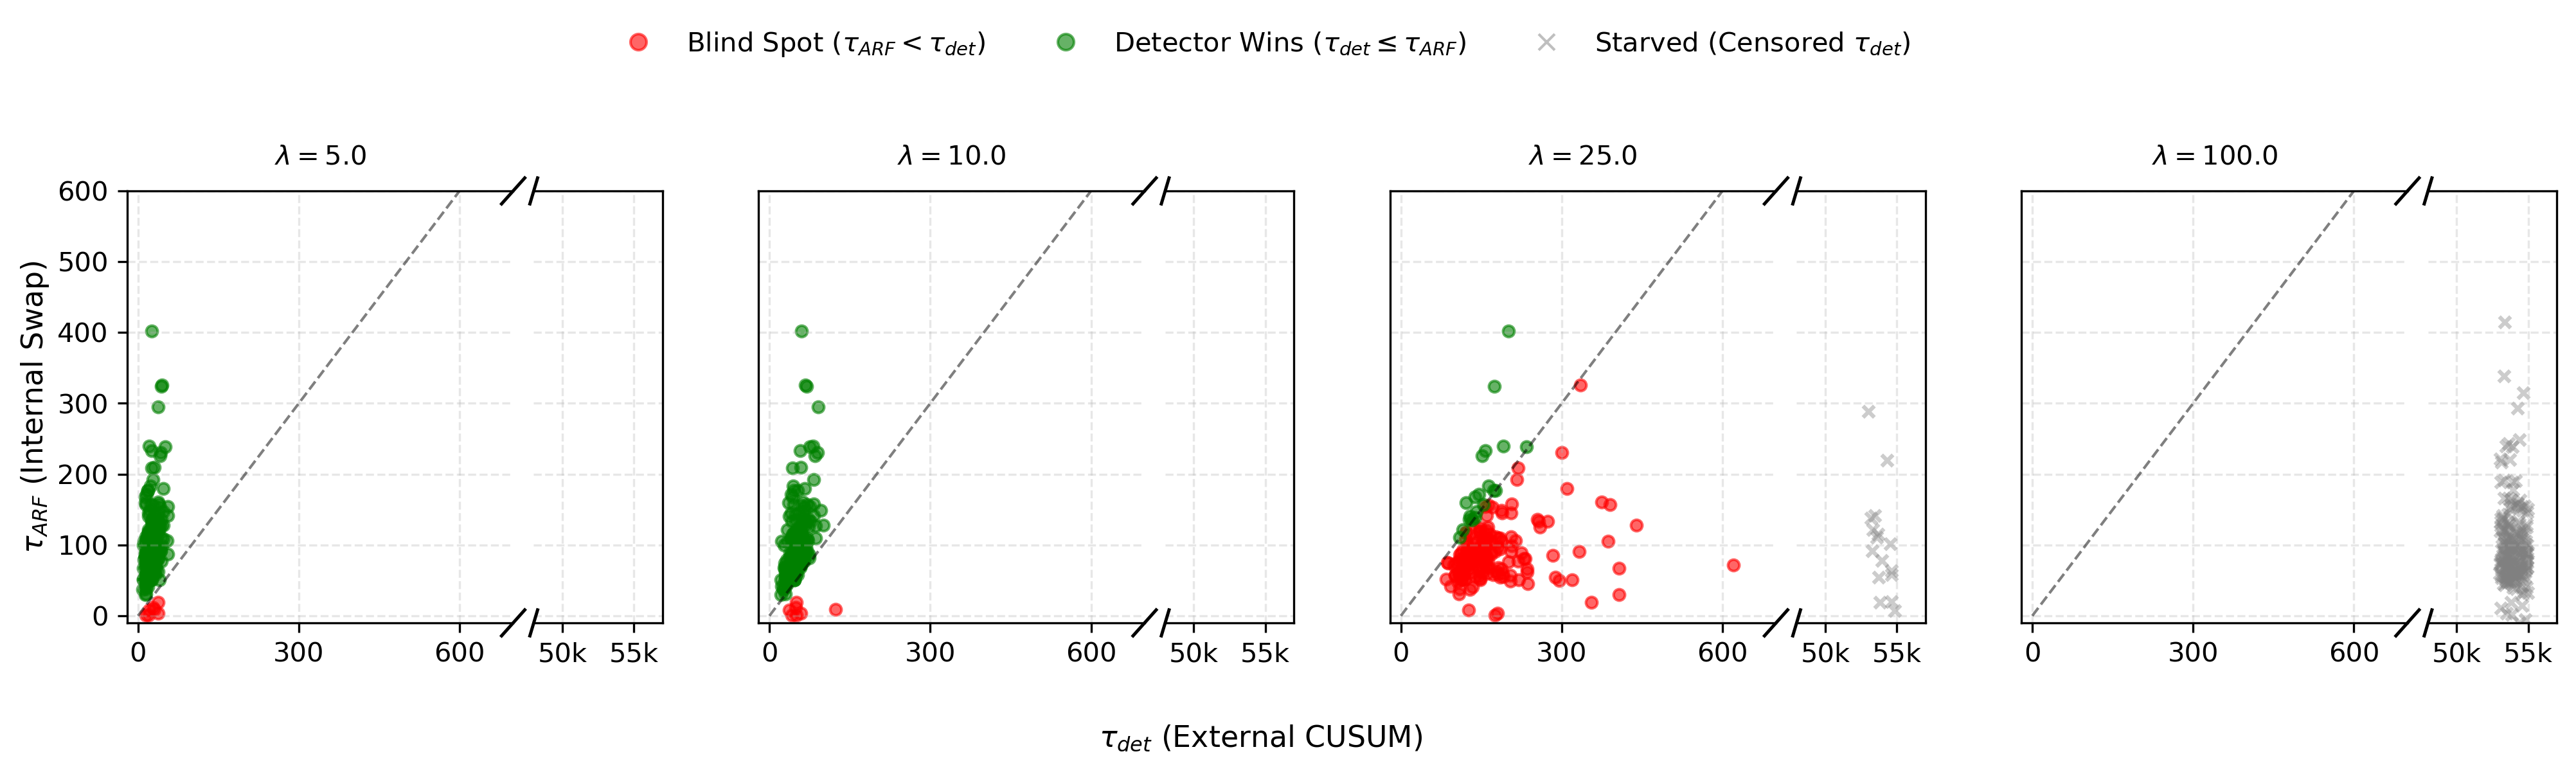
\includegraphics[width=0.90\textwidth]{Fig_R1_race_condition.png}
  \caption{First replacement ($\tau_{\mathrm{ARF}}$) against external alarm ($\tau_{\mathrm{det}}$) at $\Delta e{=}0.25$ across critical $\lambda$ ($200$ seeds/panel). \textcolor{darkgreen}{\textbf{Green}}: detector wins ($\tau_{\mathrm{det}}{\le}\tau_{\mathrm{ARF}}$). \textcolor{red}{\textbf{Red}}: first replacement before the alarm, post-recovery alarms included ($\tau_{\mathrm{ARF}}{<}\tau_{\mathrm{det}}$; labelled `Blind Spot' in the legend after the ordering of the submitted version, not Definition~\ref{def:blindspot}). \textcolor{gray}{\textbf{Gray $\times$}}: starvation ($\tau_{\mathrm{det}}$ censored at horizon $50{,}000$, offset in the broken right-hand zone). Axes: broken linear $x$, $y\le 600$. The transition $\lambda^*{\approx}15$--$25$ separates the detector-wins, replacement-first (post-recovery-dominated) and total-starvation regimes (Prop.~\ref{prop:starvation_boundary}).}
  \label{fig:race_condition}
\end{figure*}

\subsection{Regime 1: The Clock-Mismatch Artefact}\label{sec:hardware}

We isolate the impact of the evaluation clock on the real ARF across three configurations ($100$ seeds $\times$ $20$ magnitudes; Figure~\ref{fig:clock_mismatch}, Table~\ref{tab:r7_regime1}). Under \emph{mismatched} clocks ($c_{\mathrm{int}}{=}1$, $c_{\mathrm{ext}}{=}32$---River's default), the ensemble-accelerated ARF preempts the batched external ADWIN: miss rates exceed $50\%$ for $\Delta e > 0.35$ and \emph{increase} with magnitude, the counter-intuitive artefact signature. This is \emph{not} a structural ADWIN vulnerability. Under \emph{matched} clocks ($c_{\mathrm{int}}{=}c_{\mathrm{ext}}{=}1$) the external ADWIN \emph{wins} for $\Delta e > 0.30$ (miss $<5\%$; the residual $\approx 11\%$ at $\Delta e{\approx}0.19$ is the tail of the weak-signal band), because it reads the \emph{ensemble} error averaged over $M{=}10$ trees---a higher-SNR signal than any single tree (under the same clock the single-member arm stays at $30\%$ miss over that band, and $35\%$ across the full magnitude grid). The decoupled configuration ($c_{\mathrm{int}}{=}32$, $c_{\mathrm{ext}}{=}1$) confirms detection before adaptation for $\Delta e > 0.30$, consistent with the reactivity condition of Definition~\ref{def:decoupling}.

\begin{figure}[t]
  \centering
  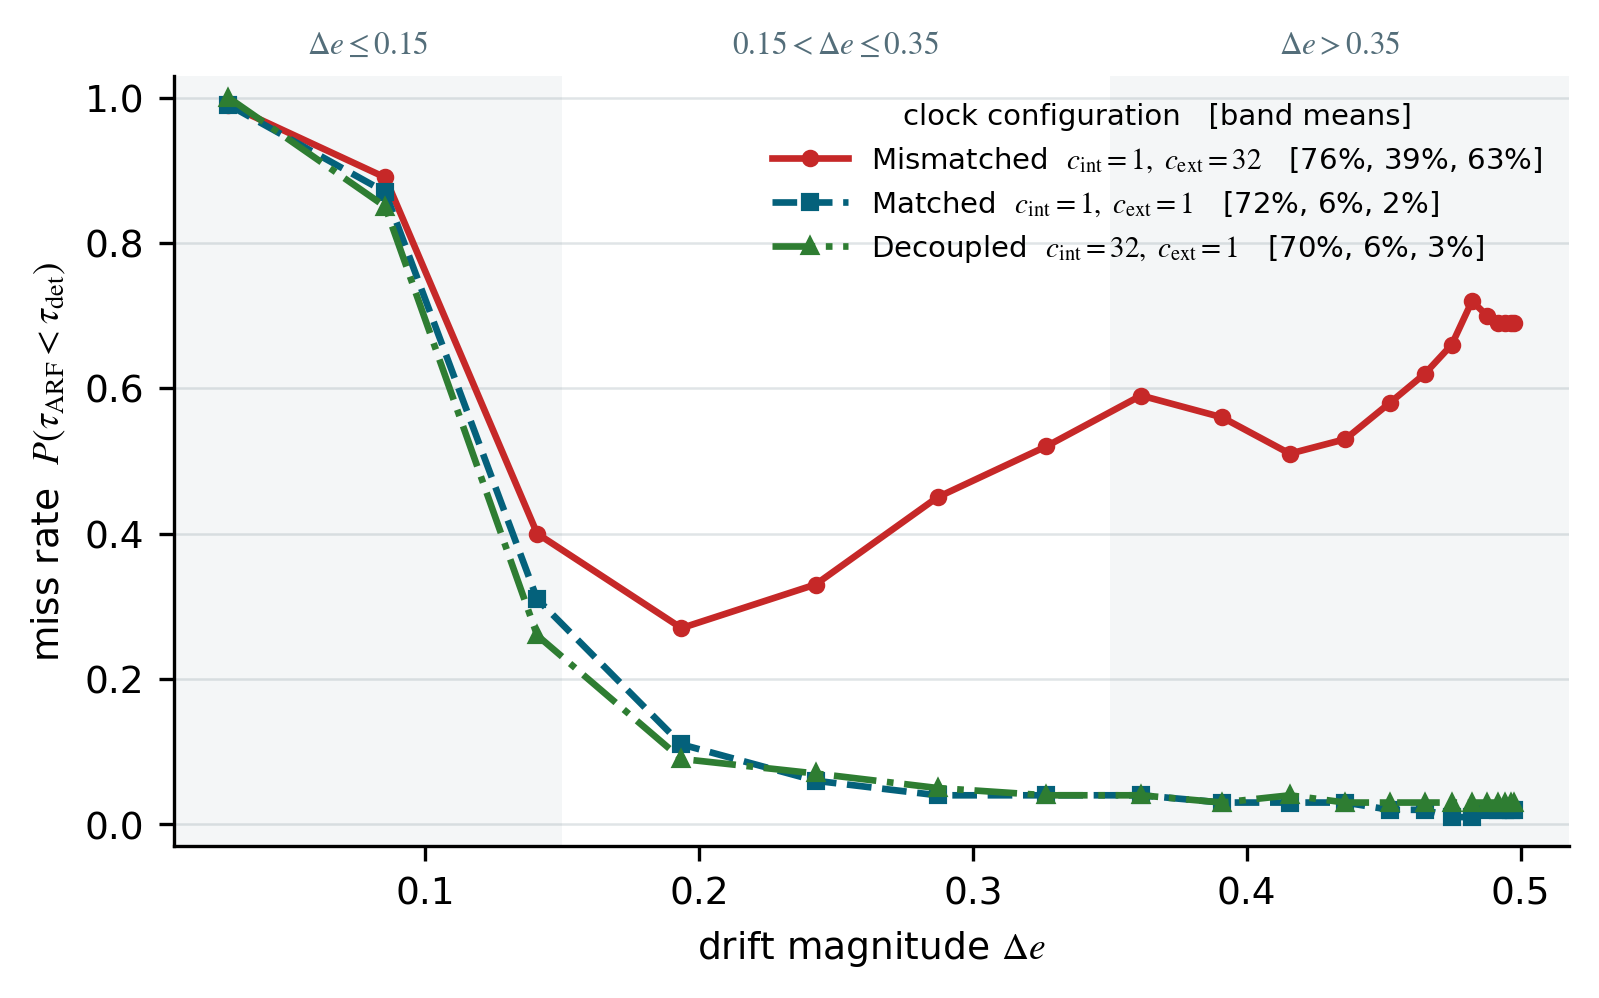
\includegraphics[width=\columnwidth]{figures/Fig_R7_clock_mismatch.png}
  \caption{Regime 1, the clock-mismatch artefact. Miss rate
    $P(\tau_{\mathrm{ARF}} < \tau_{\mathrm{det}})$ against drift magnitude for the three clock
    configurations, $100$ seeds $\times$ $20$ magnitudes. Under mismatched clocks the miss rate
    \emph{increases} with magnitude above $\Delta e \approx 0.2$; under matched and decoupled clocks
    it decays monotonically. Band means in the legend are those of
    Table~\ref{tab:r7_regime1}.}
  \label{fig:clock_mismatch}
\end{figure}

\begin{table}[t]
  \centering
  \caption{Regime 1, the clock-mismatch artefact: miss rate $P(\tau_{\mathrm{ARF}} < \tau_{\mathrm{det}})$ of the external ADWIN, averaged over three magnitude bands ($100$ seeds $\times$ $20$ magnitudes).}
  \label{tab:r7_regime1}
  \begin{tabular}{@{}lccc@{}}
  \toprule
  Clock configuration & $\Delta e \le 0.15$ & $0.15 < \Delta e \le 0.35$ & $\Delta e > 0.35$ \\
  \midrule
  Mismatched ($c_{\mathrm{int}}{=}1,\ c_{\mathrm{ext}}{=}32$) & $76\%$ & $39\%$ & $63\%$ \\
  Matched ($c_{\mathrm{int}}{=}1,\ c_{\mathrm{ext}}{=}1$) & $72\%$ & $6\%$ & $2\%$ \\
  Decoupled ($c_{\mathrm{int}}{=}32,\ c_{\mathrm{ext}}{=}1$) & $70\%$ & $6\%$ & $3\%$ \\
  \bottomrule
\end{tabular}

\end{table}

\subsection{Regime 2: Asymptotic Complexity Intersection}\label{sec:complexity}

Which family is the most exposed depends on the false-alarm level: the cumulative monitor asks the least evidence of the three families below $\ln(1/\alpha) \approx 16.3$ and the most above $\ln(1/\alpha) \approx 19.0$ (Corollary~\ref{cor:split}); at the thresholds studied here the CUSUM/PHT is starved (Section~\ref{sec:starvation}).
Figure~\ref{fig:pht_scenarios} shows the instrumented race between the real ARF ($M = 10$, $c_{\mathrm{int}} = 1$) and an external StrictCUSUM at three thresholds.

A high threshold ($\lambda = 50$) produces \emph{complete} starvation: the PHT detects in $<$1\% of runs across all $\Delta e$ (Figure~\ref{fig:pht_scenarios}A), as the ARF's ensemble-accelerated adaptation leaves less evidence than the threshold requires (Remark~\ref{rem:shortwindow}). An intermediate threshold ($\lambda = 25$) reveals partial detection at moderate $\Delta e$ but complete starvation at large $\Delta e$ (Figure~\ref{fig:pht_scenarios}B): miss rates rise from 68\% to 100\% as $\Delta e$ increases---the signature of starvation, a stronger drift missed more often. A low-threshold PHT ($\lambda = 8$) achieves a safe zone for $\Delta e > 0.15$ (Figure~\ref{fig:pht_scenarios}C), but sacrifices false-alarm robustness.

\begin{figure*}[t]
  \centering
  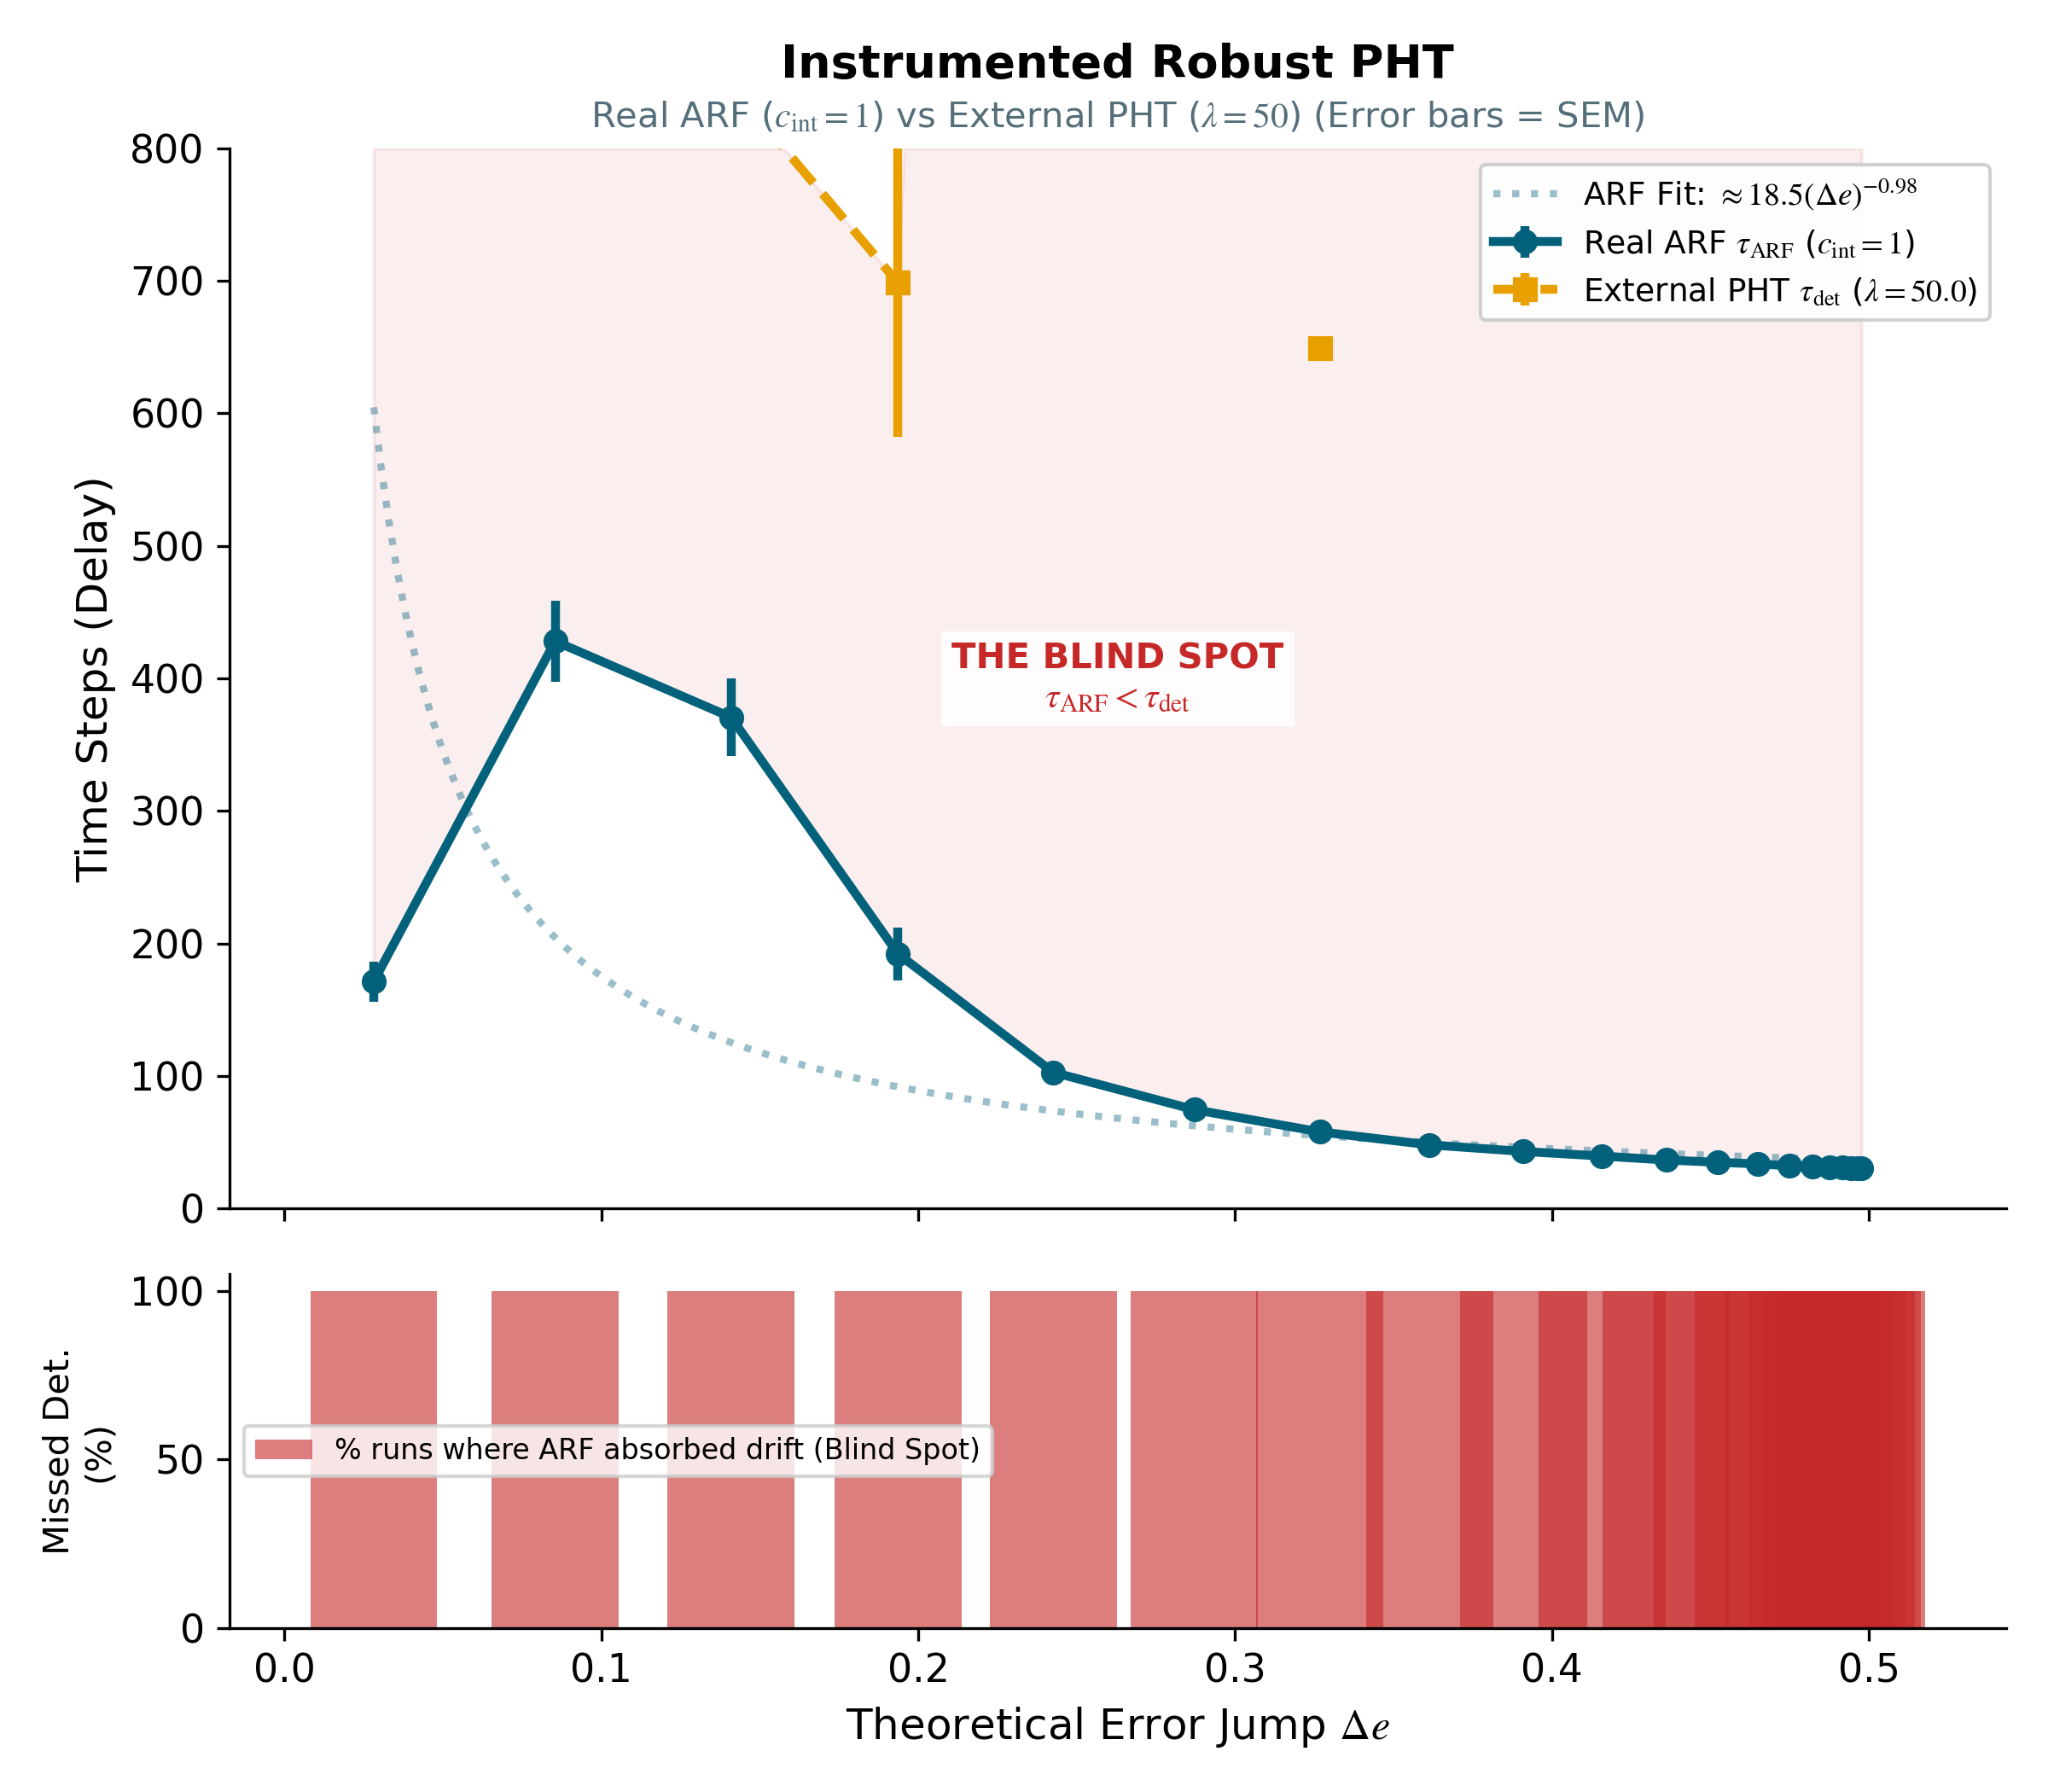
\includegraphics[width=0.31\textwidth]{Fig_R2_A_PHT_ARF.png}
  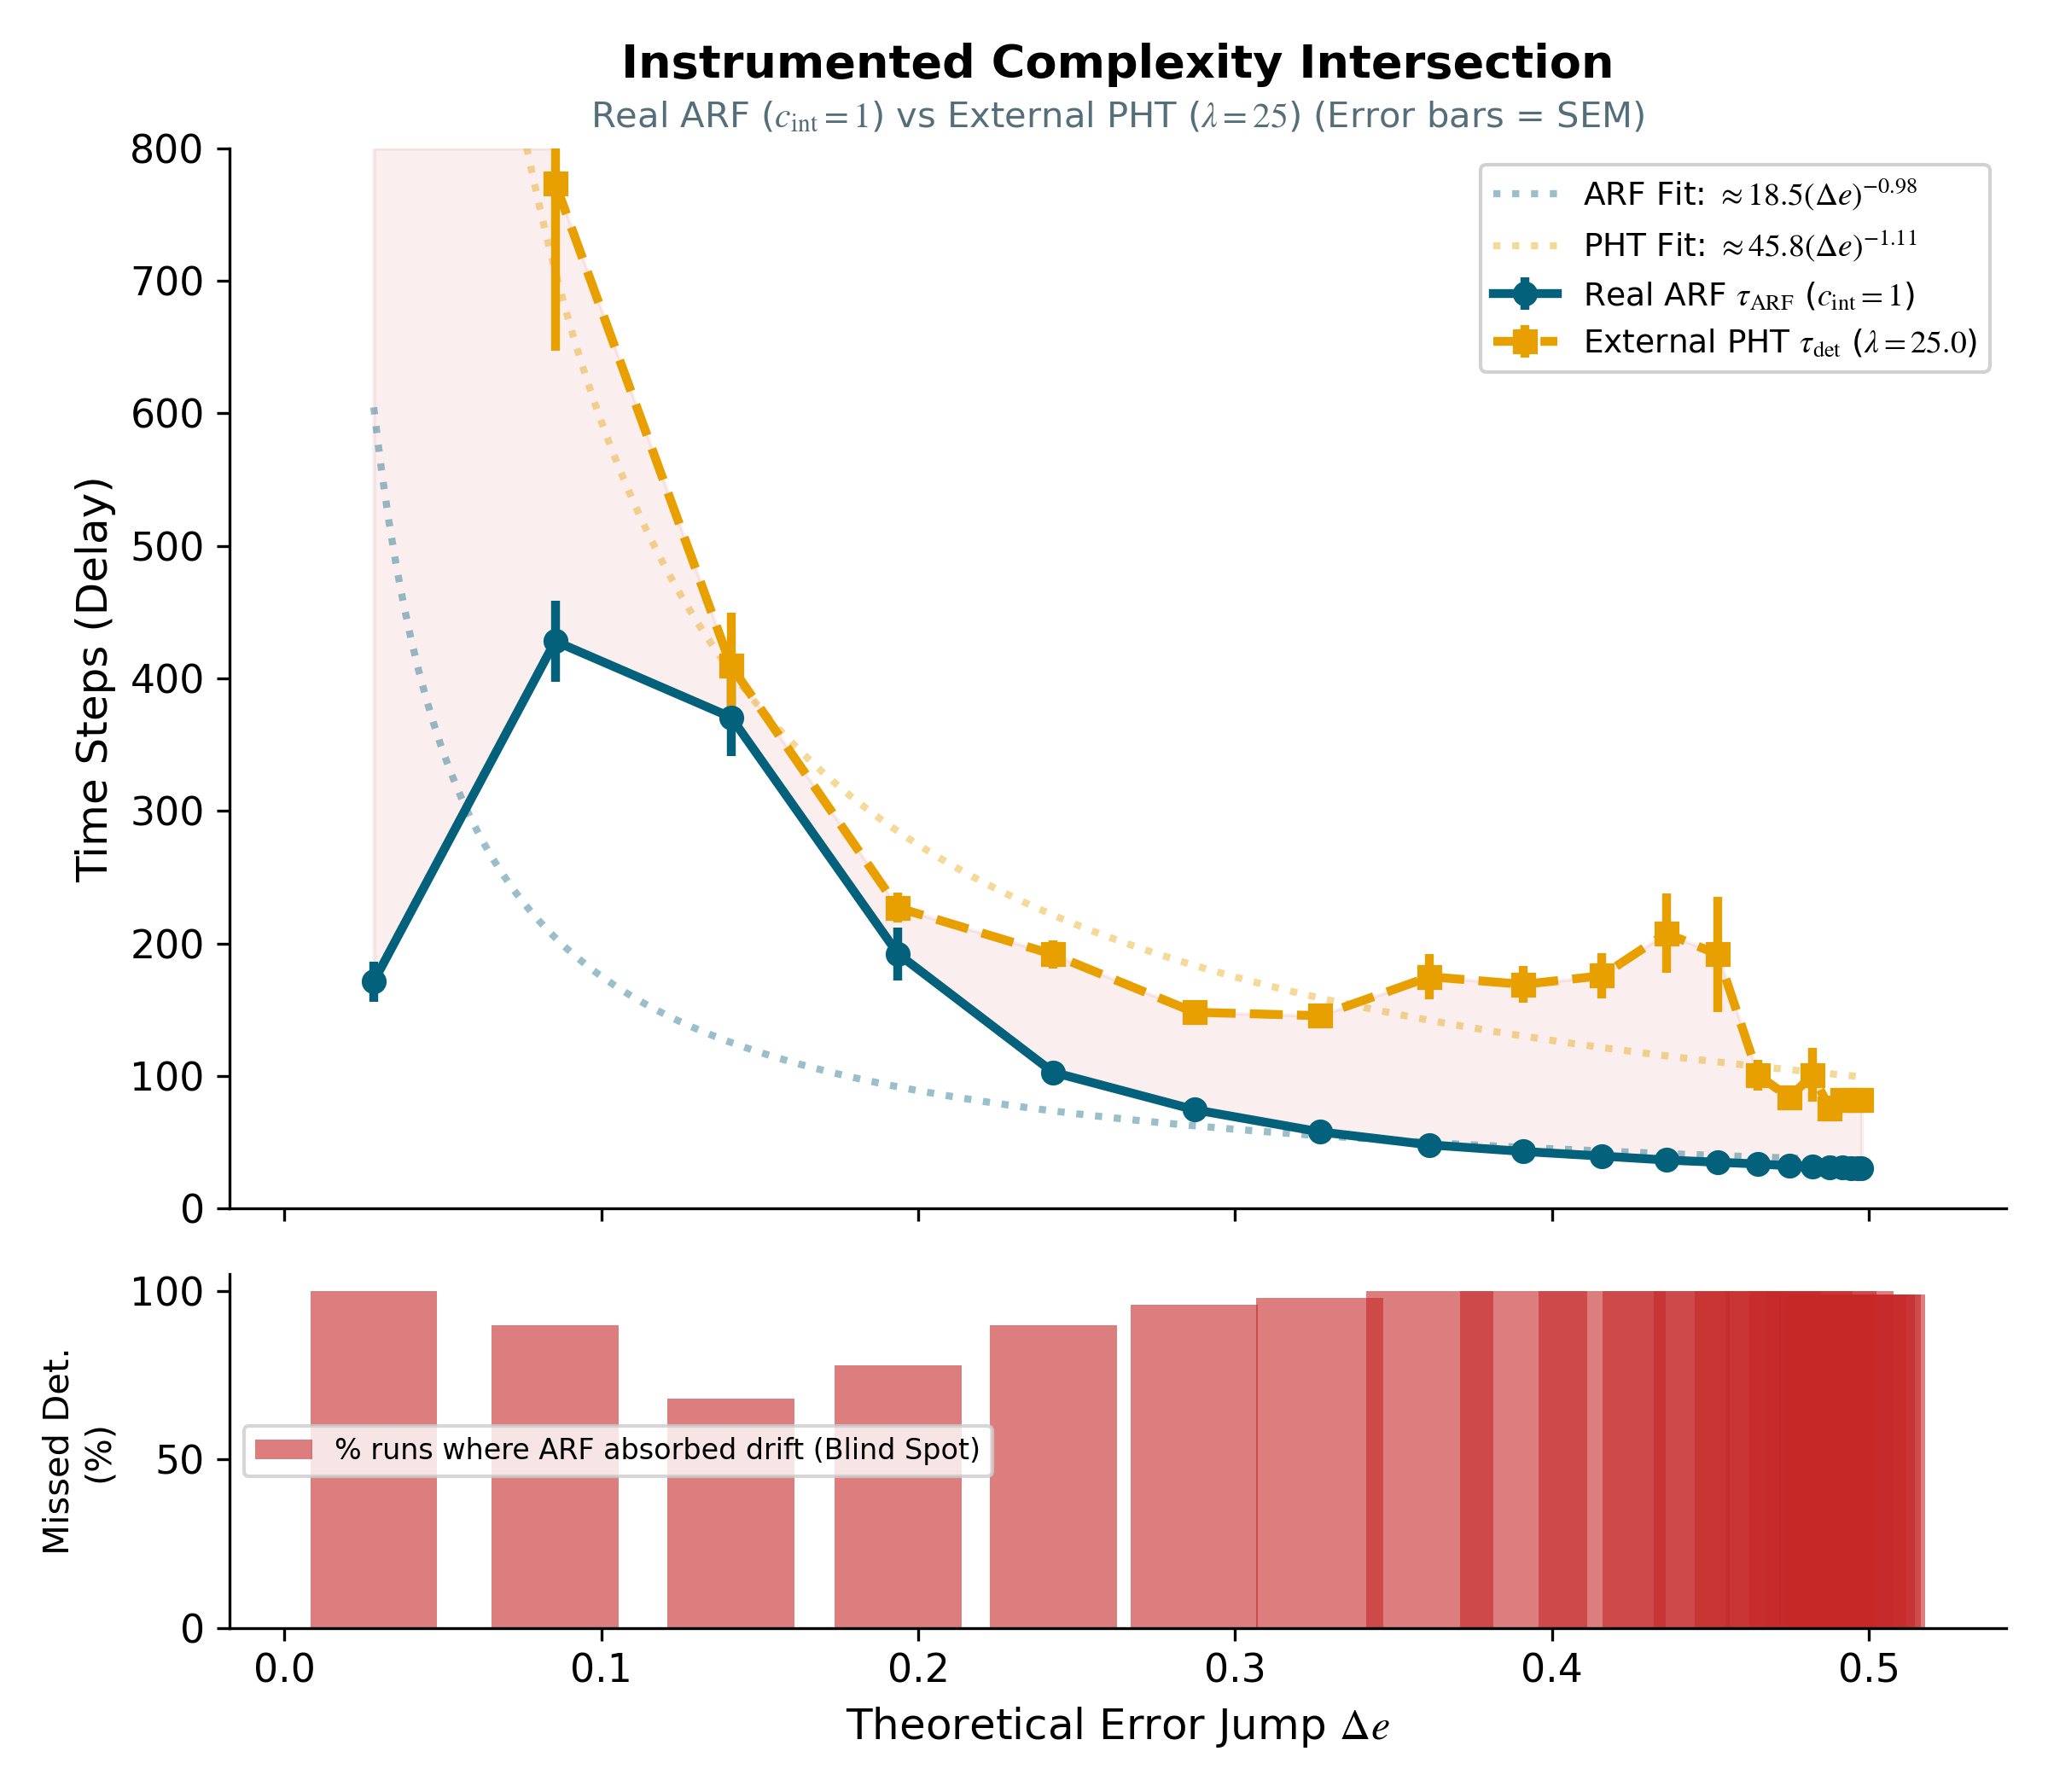
\includegraphics[width=0.31\textwidth]{Fig_R2_B_PHT_ARF.png}
  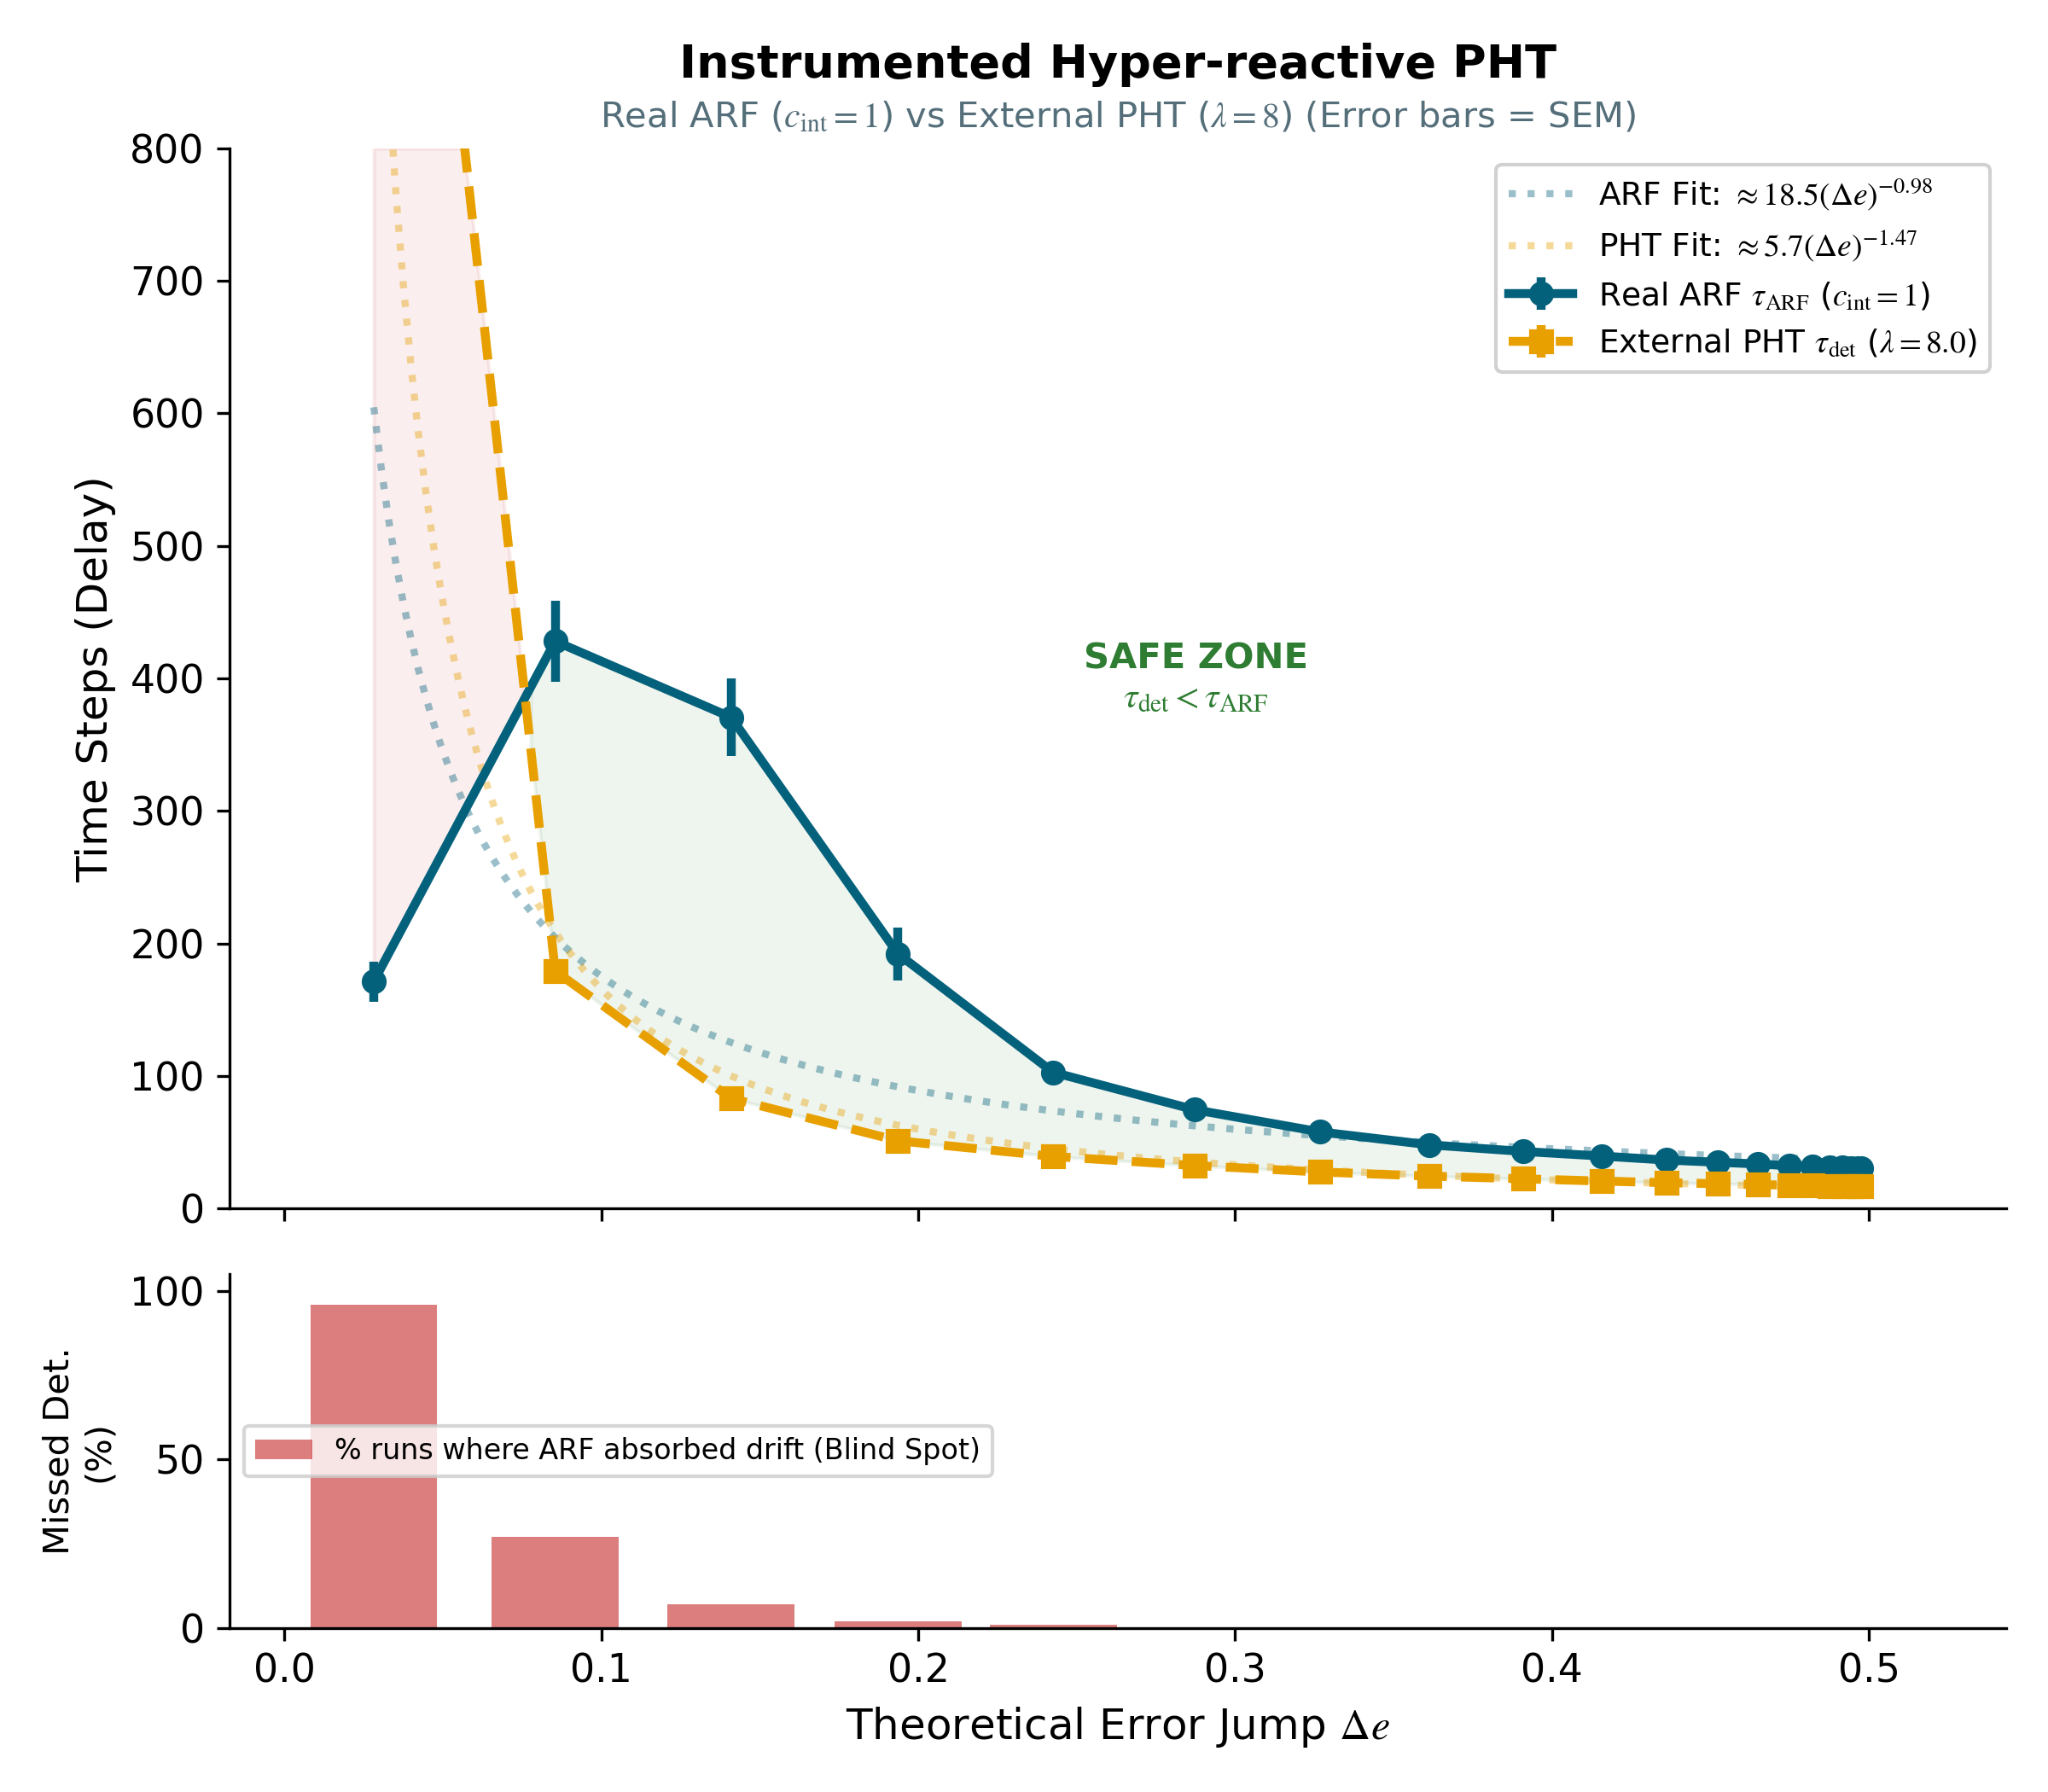
\includegraphics[width=0.31\textwidth]{Fig_R2_C_PHT_ARF.png}
  \caption{Instrumented Asymptotic Complexity: ARF ($M{=}10$) vs.\ external StrictCUSUM (ARF fit $\approx 18.5(\Delta e)^{-0.98}$ vs.\ HAT $\approx 102(\Delta e)^{-1.02}$; ensemble onset acceleration converts partial into total starvation). (A)~$\lambda{=}50$: $100\%$ miss. (B)~$\lambda{=}25$: misses increasing with $\Delta e$. (C)~$\lambda{=}8$: safe zone at $\Delta e{>}0.15$. The shaded `Blind Spot' region and bars mark the ordering $\tau_{\mathrm{ARF}}{<}\tau_{\mathrm{det}}$, not Definition~\ref{def:blindspot}.}
  \label{fig:pht_scenarios}
\end{figure*}

\begin{remark}[Exponent revision]\label{rem:exponent}
  The instrumented experiments yield $\hat\alpha_{\mathrm{ARF}} \approx 0.98$ and $\hat\alpha_{\mathrm{HAT}} \approx 1.02$, both consistent with $\mathcal{O}(1/\Delta e)$ rather than the Hoeffding bound $\mathcal{O}((\Delta e)^{-2})$.
  This discrepancy arises because the Hoeffding bound governs sub-window splitting, while real tree-swap dynamics involve warning phases, background-tree pre-training, and Poisson-weighted bootstrap---mechanisms that accelerate adaptation beyond the concentration inequality.
  The ordering $\tau_{\mathrm{ARF}} < \tau_{\mathrm{det}}$ survives the shared exponent: onset acceleration reduces $K_{\mathrm{ARF}}$ by at least $4.1$--$8.0\times$ relative to a single tree (censoring-aware lower bounds, $95\%$ CIs $[3.45, 4.96]$ and $[6.40, 9.72]$; Section~\ref{sec:hydra}), compensating for the shared exponent.
\end{remark}

\begin{remark}[Background swap rate]\label{rem:bgswap}
  At very low drift magnitudes ($\Delta e < 0.10$), $\tau_{\mathrm{ARF}}$ exhibits non-monotonic behavior: the ARF occasionally swaps trees even under stationarity due to the high sensitivity of ADWIN at $c = 1$.
  These ``noise swaps'' produce artifactually short $\tau_{\mathrm{ARF}}$ values and carry essentially no information about recovery in the weak band: for $\Delta e \le 0.15$ the first swap correlates with the error-recovery times at Spearman $0.06$ ($\tau_{\mathrm{err}}(0.50)$) and $0.10$ ($\tau_{\mathrm{err}}(0.10)$), against $0.850$ and $0.694$ over the whole grid. They are not the adaptation event, and they are not evidence of erasure.
\end{remark}

\begin{remark}[False-alarm flooding: the non-stationary dual of starvation]\label{rem:flooding}
  Starvation and flooding are duals in their effect on $F_1$, not two faces of one cause. Starvation is the erasure of a genuine transient, and the $\tau^*$-anchored decomposition assigns $\LearnSharePure\%$ of that erasure to ordinary incremental learning with no tree replaced (Remark~\ref{rem:first_swap}) rather than to the internal clock: the internal ADWIN at $c_{\mathrm{int}}{=}1$ fixes \emph{when} adaptation starts, not \emph{what} removes the evidence. Flooding has a different mechanism, and the two should not be attributed to one root cause.

  Read through $\mathrm{ARL}_0$, an alarm raised after the transient is uninformative and arrives under the no-change law at rate $1/\mathrm{ARL}_0$ (Remark~\ref{rem:sufficient}). At the measured base rate $p_0 = \PzeroMeas$ with $\delta_P = \DeltaPtext$ that rate is negligible---$\mathrm{ARL}_0 = \ArlFifteen$ steps at $\lambda = \LambdaFA$---and it accounts for essentially none of the alarms observed: on \emph{gradual\_balanced} it predicts $3\times10^{-3}$ alarms over the armed pre-change span against $86$ measured, short by a factor $\FloodArlGap$. The flooding alarms are not null-regime false alarms, and no recalibration of $\mathrm{ARL}_0$ explains them.

  What produces them is the post-change regime itself. The error rate does not return to its pre-change level on that stream ($0.50$ against $0.058$ for the ARF pipeline), so a monitor re-armed after each alarm crosses $\lambda$ again roughly every $\lambda / (\bar e_{\mathrm{post}} - p_{\mathrm{pre}} - \delta_P)$ steps. That re-arm model, with no fitted constant, returns $\FloodPredArf$ alarms for PHT$+$ARF($c{=}1$) against $86$ measured and $\FloodPredHt$ for PHT$+$HT against $7$, and their ratio $7.6\times$ against a measured $12.2\times$. We claim order-of-magnitude agreement only: Sections~\ref{sec:proteus} and~\ref{sec:crossover} run River's adaptive mean-tracking PageHinkley at $\delta_P = 0.005$, not the fixed-$p_0$ recursion of Eq.~\eqref{eq:cusum}, so this is a consistency check across estimators and is labelled as one. The asymmetry between the two pipelines is a threshold asymmetry, and it is an artefact of where the false-alarm budget is measured. The one-false-alarm-per-warm-up calibration hands the ARF $\FloodLamArf$ and the HT $\FloodLamHt$, a factor of $6.3$; but the warm-up is $10\%$ of the stream while the detector then runs armed over a pre-change span $\SpanOverWarm$ times longer, and over that span the two nominally equal budgets buy $\FaSpanArf$ alarms for the ARF against $\FaSpanHt$ for the HT. Re-calibrating each pipeline to one expected false alarm over the span it actually runs gives $\LamEqArf$ and $\LamEqHt$, and the $F_1$ ratio falls from $\RhoRefMeas$ to $\RhoEqSpan$ $\RhoEqSpanCI$ (seed-paired bootstrap): $\ThresholdShare\%$ of the published log-ratio is threshold-attributable and the residual coupling effect is a factor $\RhoEqSpan$, small but with a confidence interval excluding $1$. Nor does the asymmetry reflect a variance property of bagging: it is largest exactly where the calibration window is shortest---the two classifiers have least converged there---and on the other two INSECTS variants, whose warm-ups are two and three times longer, the ordering reverses and the ARF receives the \emph{higher} threshold. What floods is not the adaptive classifier but a threshold set on a window too short to represent the regime the monitor will run in. Flooding remains parametrically controllable---alarms scale as $1/\lambda$ in the re-arm model---whereas starvation is structural: no CUSUM threshold escapes it (Section~\ref{sec:starvation_boundary}).
\end{remark}

\subsection{Theoretical Bounds: The Starvation Boundary}\label{sec:starvation_boundary}

Onset acceleration (Section~\ref{sec:hydra}) and starvation (Section~\ref{sec:starvation}) combine into a boundary on the viability of external monitoring.
We bound the probability of missed detection without any dependence hypothesis, and show that no critical ensemble size follows from that bound (Corollary~\ref{cor:mcrit}): a reliability target $r$ is settled on the measured race instead.

\paragraph{Dependence: what the bound needs.}
The $M$ trees in the ARF are trained on the \emph{same} data stream via Poisson-weighted bootstrap (Oza bagging with $\lambda = 6$~\cite{gomes_arf_2017}), so the individual detection delays $\tau_1, \ldots, \tau_M$ are \emph{positively correlated}: a drift that is easy for tree $i$ to detect is also easy for tree $j$.
Positive correlation is not enough to license the independence formula as an upper bound. What that formula needs is positive \emph{association of the events} $\{\tau_i \le s\}$ at the level $s$, i.e.\ $\mathbb{P}(\tau_i \le s,\ \tau_j \le s) \ge F(s)^2$, and an exchangeable pair with $\mathrm{Corr}(\tau_1,\tau_2) = +0.51$ can fail it: placing mass $0.3$ on each of $(1,100)$ and $(100,1)$ and $0.2$ on each of $(2,2)$ and $(200,200)$ gives $F(2) = 0.5$ but $\mathbb{P}(\min \le 2) = 0.80 > 0.75 = 1 - [1-F(2)]^2$.
What does license it is the \emph{common-factor} structure --- conditional independence of the $\tau_i$ given the shared stream, which yields the direction by Jensen's inequality --- and that is a hypothesis about River's implementation, not a corollary of shared training data. Instrumenting the forest generator refutes its positional precondition: River threads one generator through all $M$ trees, the Oza weight is a rejection loop whose cost is itself random ($1$--$16$ draws per tree and step, mean $7.07$), and perturbing one tree's state displaces $9{,}839$ of the draw positions consumed by the others.
We therefore state the boundary below in a form that needs \emph{no} dependence hypothesis, and our claims rest on the directly measured adaptation time $\tau_{\mathrm{ARF}}$ (Section~\ref{sec:hydra}), not on the independence formula. Appendix~\ref{sec:dependence} gives the counterexample, the generator gate, the plug-in refutation and the competing-risks form in full.

\begin{proposition}[Starvation Boundary]\label{prop:starvation_boundary}
  Let $\tau_1, \ldots, \tau_M$ denote the internal detection delays of the $M$ trees in the ARF, and let $F$ denote the marginal CDF of a single $\tau_i$ \emph{inside the ensemble}.
  Write $P_{\mathrm{miss}}(s) := \mathbb{P}(\tau_{\mathrm{ARF}} \le s)$ for the probability that the ensemble has already adapted by a level $s$, so that the external monitor accumulates against an error stream the classifier has removed.
  Then, for every $s$ and \emph{whatever} the dependence structure of the $\tau_i$,
  \begin{equation}\label{eq:pmiss}
    F(s) \;\le\; P_{\mathrm{miss}}(s) \;\le\; \min\bigl(1,\, M\,F(s)\bigr)\,,
  \end{equation}
  and both ends are attained, so the envelope cannot be tightened without a dependence hypothesis.
  If in addition the $\tau_i$ are exchangeable and conditionally independent given the shared data stream, the upper end may be replaced by the tighter $1 - \bigl[1 - F(s)\bigr]^M$.
\end{proposition}

\begin{proof}
  By Eq.~\eqref{eq:hydra}, $\tau_{\mathrm{ARF}} = \min_{1 \le i \le M} \tau_i$, so with $A_i := \{\tau_i \le s\}$ the event $\{\tau_{\mathrm{ARF}} \le s\}$ is $\bigcup_{i} A_i$.
  Monotonicity gives $\mathbb{P}(\bigcup_i A_i) \ge \mathbb{P}(A_1) = F(s)$; sub-additivity gives $\mathbb{P}(\bigcup_i A_i) \le \sum_i \mathbb{P}(A_i) = M F(s)$, and a probability is at most $1$. The two ends are the Fr\'echet--Hoeffding pair for a union of $M$ equiprobable events, hence attained.
  For the conditional statement, write $\mathcal{S}$ for the $\sigma$-field of the shared stream and $G := \mathbb{P}(\tau_i > s \mid \mathcal{S})$, which does not depend on $i$ by exchangeability. Conditional independence gives $\mathbb{P}(\tau_{\mathrm{ARF}} > s \mid \mathcal{S}) = G^M$, and since $x \mapsto x^M$ is convex on $[0,1]$, Jensen's inequality and the tower property give
  \[
    \mathbb{P}(\tau_{\mathrm{ARF}} > s) = \mathbb{E}\bigl[G^M\bigr] \;\ge\; \bigl(\mathbb{E}[G]\bigr)^M = \bigl[1 - F(s)\bigr]^M\,,
  \]
  which is the tighter upper end after complementation. Proposition~\ref{prop:starvation} supplies the sufficient condition under which an ensemble that has adapted by $s$ starves the external CUSUM; this proposition bounds the probability of that event.
\end{proof}

\begin{corollary}[Ensemble size is not certifiable from the envelope]\label{cor:mcrit}
  For a reliability target $r = 1 - P_{\mathrm{miss}}$, inverting Eq.~\eqref{eq:pmiss} in $M$ gives the critical ensemble size
  \begin{equation}\label{eq:mcrit}
    M_{\mathrm{crit}} = \left\lfloor \frac{\ln r}{\ln\!\bigl[1 - F(s)\bigr]} \right\rfloor\,,
  \end{equation}
  \emph{but only for the conditional form} of Eq.~\eqref{eq:pmiss}. The distribution-free upper end saturates as soon as $M F(s) \ge 1$, and in the saturated region $\min(1, M F(s))$ does not depend on $M$ at all: no ensemble size, $M = 1$ included, is certified at any target $r < 1$. At $M = 10$ saturation begins at $F(s) \ge 0.10$, which covers the entire operating range of this work. Eq.~\eqref{eq:mcrit} is therefore not available as a design rule, and the reliability $r$ must be settled empirically.
\end{corollary}

\paragraph{Retraction of the single-tree instantiation.}
Earlier versions evaluated Eq.~\eqref{eq:mcrit} with $F$ read from the empirical CDF $\widehat{F}$ of the single-tree delays $\tau_{\mathrm{HAT}}$ ($M = 1$), obtaining at $\Delta e = 0.33$, $\lambda = 50$: $\mathbb{E}[\tau_{\mathrm{HAT}}] = 463$, $\widehat{F}(158) = 0.49$ and $M_{\mathrm{crit}} = 0$ at $r = 0.95$. Those numerals reproduce, but the substitution $F = \widehat{F}$ does not survive measurement. A standalone HAT is not a tree inside the ARF---Poisson weighting and a one-feature split rule make the ensemble member's delay law strictly more dispersed---and over the $80$ testable cells of the instrumented grid ($20$ magnitudes $\times$ $\lambda \in \{8, 15, 25, 50\}$ at $M = 10$, $\SixSeeds$ runs each) the plug-in upper end falls \emph{below} the Wilson $95\%$ lower end of the measured $P_{\mathrm{miss}}$ in $10$ of them. The mechanism is the left tail: at $\Delta e = \SixCanonDeltaE$ the fastest of $\SixSeeds$ HAT runs adapts at step $33$, so $\widehat{F}$ vanishes below that, while $4$ of $\SixSeeds$ ARF runs have already adapted by step $25$; symmetrically, the slowest member is up to twice as slow as $\widehat{F}$ predicts. The instantiation is retracted rather than recomputed.
The ensemble claim rests instead on the measured race. Treating adaptation and detection as competing risks under the common administrative horizon $t_c = 4000$ post-drift steps, the external monitor at $\lambda = 50$ wins \emph{none} of the $2{,}000$ instrumented runs: $\mathbb{P}(\tau_{\mathrm{ARF}} < \tau_{\mathrm{det}}) = 1$ with a paired bootstrap band of $[1.00, 1.00]$ at every magnitude, which is the ${<}1\%$ detection rate of Figure~\ref{fig:pht_scenarios}(A) read as a race rather than as a threshold comparison. Finally, a Kolmogorov--Smirnov test with parametric bootstrap ($N{=}2000$, rate refitted on each replicate) rejects an exponential fit of $\tau_{\mathrm{HAT}}$ at all twenty magnitudes (largest $p = 0.0030$): the $M$-fold identity invoked in Section~\ref{sec:hydra} is a calibration reference for the exponential family, not a property of the measured delay law.

\subsection{The Reactivity Condition}\label{sec:decoupling}

\begin{definition}[Reactivity condition, reliability form]\label{def:decoupling}

  \smallskip
  \emph{(i)~Formal condition.} Fix an operational envelope $\mathcal{E} = [\Delta e_{\min}, \Delta e_{\max}]$ and a reliability level $1-\alpha$. A monitoring pipeline is \textbf{$(1-\alpha)$-decoupled on $\mathcal{E}$} if
  \begin{equation}\label{eq:decoupling}
    \Pr\bigl(\tau_{\mathrm{det}} \le W_{\mathrm{argmax}}\bigr) \;\ge\; 1-\alpha
    \qquad \text{for every } \Delta e \in \mathcal{E}\,.
  \end{equation}
  The condition compares the detection delay with the erasure delay. It carries no clock parameter and no threshold, and is therefore stated in terms shared by every detector family.

  \smallskip
  \emph{(i-bis)~Certificate for the cumulative-evidence family.} Let $q_\alpha(\Delta e)$ denote the $\alpha$-quantile of the evidence ceiling $A_{\mathrm{swap}}$ at magnitude $\Delta e$. By Proposition~\ref{prop:certificate}, $A_{\mathrm{swap}} \ge \lambda$ forces a crossing at or before $\tau^* + W_{\mathrm{argmax}}$; hence $\lambda \le \lambda_{\mathrm{op}}(\alpha, \mathcal{E}) := \min_{\Delta e \in \mathcal{E}} q_\alpha(\Delta e)$ is sufficient for $(1-\alpha)$-decoupling on $\mathcal{E}$. The certificate is sufficient, not necessary: a pipeline violating it may still detect, through a fluctuation of $S_t$ above $A_{\mathrm{swap}}$ or because its stopping time is not governed by $\lambda$ at all. ADWIN paired with the ARF detects reliably at $c_{\mathrm{ext}} = c_{\mathrm{int}}$ for the second reason. That configuration is consistent with~\eqref{eq:decoupling} and was not with the strict biconditional of the submitted version, which we withdraw.

  \smallskip
  \emph{(ii)~Operational calibration.} Condition~\eqref{eq:decoupling} is existential and circular as stated. The following procedure renders it constructive over an operational envelope $[\Delta e_{\min}, \Delta e_{\max}]$ of drift magnitudes to be guaranteed at reliability $1-\alpha$:

  \textbf{(1)}~Fix the operational envelope $[\Delta e_{\min}, \Delta e_{\max}]$. \textbf{(2)}~For each $\Delta e$ on a grid spanning the envelope, inject a synthetic abrupt drift into the ARF during offline calibration and record the empirical distribution of internal adaptation times $\tau_{\mathrm{ARF}}(\Delta e)$. \textbf{(3)}~Extract the empirical $\alpha$-quantile $q_{\alpha}(\tau_{\mathrm{ARF}}(\Delta e))$ at each grid point. \textbf{(4)}~Record the evidence ceiling $A_{\mathrm{swap}}$ of each calibration run and set $\lambda_{\mathrm{op}} := \min_{\Delta e} q_{\alpha}\bigl(A_{\mathrm{swap}}(\Delta e)\bigr)$. The rectangular surrogate $q_{\alpha}(\tau_{\mathrm{ARF}})\cdot(\Delta e - \delta_P)$ used in the submitted version assumes a constant accumulation rate over a transient of length $\tau_{\mathrm{ARF}}$; synchronised instrumentation invalidates both halves of that assumption and the surrogate is withdrawn. Step~(4) requires no extra simulation: $S_t$ recomputes offline from the recorded error stream for any $\lambda$ and any $\delta_P$.

\begin{empresult}[Envelope dependence of the admissible set]\label{res:tension}
  With $\lambda_{\mathrm{FA}} = \LambdaFA$ as the declared false-alarm threshold of Section~\ref{sec:proteus} and $\alpha = 0.05$, the measured ceiling gives $q_{0.05} = \QlowFloorLo$ at $\Delta e = \DeFloorLo$ and $\QlowFloorHi$ at $\Delta e = \DeFloorHi$. The admissible set $\{\lambda \ge \lambda_{\mathrm{FA}}\} \cap \{\lambda \le \lambda_{\mathrm{op}}\}$ is therefore empty for every envelope floored at or below $\DeFloorLo$ and non-empty for every envelope floored at or above $\DeFloorHi$. The detectability floor $\Delta e_c := \inf\{\Delta e : q_{0.05}(\Delta e) \ge \lambda_{\mathrm{FA}}\}$ lies strictly inside that interval, at $\Delta e_c = \DeCrit$ ($95\%$ bootstrap CI $\DeCritCI$, $n=300$). Standard synthetic benchmarks operate below it, which is why the failure mode does not surface on them.
\end{empresult}

\begin{remark}[Envelope truncation]\label{rem:envelope}
  The magnitude grid is uniform in the boundary shift $b$ and therefore strongly non-uniform in $\Delta e$: seven of its twenty points fall in $\Delta e \in [0.475, 0.498]$, where the post-change class prior $\Pr(y=1) = 0.5 - \Delta e$ drops below $2.5\%$ and the post-change concept is close to constant. Over an untruncated envelope the minimum defining $\lambda_{\mathrm{op}}$ is attained inside that cluster and measures the generator rather than the pipeline. Truncation is not a stylistic choice: a seed-level bootstrap of $\min_{\Delta e} q_{0.05}$ over $[\EnvLo, 0.50]$ places the estimate below $\lambda_{\mathrm{FA}}$ in $\WideEnvUnstable\%$ of $10{,}000$ replicates, so the untruncated calibration is not identified at this sample size. We therefore floor the operational envelope at $\EnvLo$ and cap it at $\EnvHi$, where the prior remains at $10\%$; there the certificate is stable, $\lambda_{\mathrm{op}} = \LambdaOpNarrow$ with bootstrap interval $\LambdaOpNarrowCI$ and no replicate below $\lambda_{\mathrm{FA}}$.
\end{remark}

  The minimum over the envelope (rather than evaluation at $\Delta e_{\min}$ alone) is mandatory because $q_{\alpha}(\tau_{\mathrm{ARF}})$ is \emph{non-monotone} in $\Delta e$: a fine-magnitude sweep ($\Delta e \in [0.10,0.50]$, $200$ seeds, $\alpha = 0.05$) run at $T_{\mathrm{drift}} = 2000$ shows $q_{0.05}$ to be magnitude-\emph{independent} (constant at $12.95$) for $\Delta e \le 0.16$. That plateau is a property of the \emph{warm-up}, not of the ARF: repeating the identical sweep at $T_{\mathrm{drift}} = 4000$ dissolves it, $q_{0.05}$ rising $25.70 \to 30.95 \to 54.70 \to 54.70$ over the same four magnitudes. The floor is therefore a guard against an immature ensemble---not, as we previously argued, a signature of noise-driven swaps (Remark~\ref{rem:bgswap})---and it must be re-derived for the warm-up actually deployed. The procedure requires only offline simulation of the target drift, bypassing analytical estimation of $K_{\mathrm{ARF}}$ and $F$.
\end{definition}

Default River configurations use $c_{\mathrm{int}} = 1$ and $c_{\mathrm{ext}} = 32$, violating Definition~\ref{def:decoupling} and producing the worst-case clock-mismatch artefact (Section~\ref{sec:hardware}).

For cumulative-evidence monitors, one alternative is to deploy a \textbf{non-adaptive classifier} (e.g., Hoeffding Tree): with no internal drift mechanism there is no replacement for the accumulation to compete with, and on ProteuS the HT arm detects $932/1080$ drifts where the ARF arm detects none (Table~\ref{tab:results_concept}). That is a measurement on the tested configurations, not a guarantee by construction.

% docs/manuscript/sections/protocol_v2.tex
% Experimental protocol: the resampling unit of every confidence interval, the inter-seed
% aggregation rule, the treatment of the 12 ProteuS transitions, the complete hyper-parameter set,
% the multiplicity policy, the complete separations, the seed-paired bootstrap and the per-worker
% PRNG lock. Every value below is quoted from a committed artifact or from a source line.

\section{Experimental Protocol}\label{sec:protocol}

This section states, for every interval and every test reported in
Section~\ref{sec:experiments}, what was resampled, what was pooled and what was held fixed. The
answer is not uniform across the paper, and it is not presented as if it were.

\subsection{Resampling Unit of Each Confidence Interval}\label{sec:protocol_ci}

Five distinct resampling units appear in the paper. Table~\ref{tab:protocol_ci} names each one
with its replicate count, its seed and its generator.

\begin{table*}[t]
  \centering
  \caption{Resampling unit of every confidence interval reported in this paper. The unit is not
  uniform: it is the seed wherever arms are seed-paired, the per-drift jump where the estimand is
  itself a per-drift quantity, and parametric where the null is a fitted family. Every generator is
  a locally injected \texttt{numpy.random.Generator}; no bootstrap draws from the global NumPy
  state.}
  \label{tab:protocol_ci}
  \small
  \begin{tabular}{@{}p{0.27\textwidth}p{0.24\textwidth}rlp{0.14\textwidth}@{}}
    \toprule
    \textbf{Statistic} & \textbf{Resampling unit} & \textbf{$n_{\mathrm{boot}}$} & \textbf{Seed} & \textbf{Generator} \\
    \midrule
    Table~\ref{tab:results_concept} F1 and ADD; $\alpha$-sweep & seed index, paired across arms & 1000 & 12345 & local \texttt{default\_rng} \\
    Onset acceleration $\gamma_M$ (RMST ratio $\tau_{\mathrm{HAT}}/\tau_{\mathrm{ARF}}$) & seed index, paired across arms & 10000 & 20260906 & local \texttt{default\_rng} \\
    Evidence ceiling, $\lambda_{\mathrm{op}}$, $\Delta e_c$ & seed, paired and unpaired variants & 10000 & 12345 & local \texttt{default\_rng} \\
    $\Delta e$ on real streams (Table~\ref{tab:real_data_summary}) & the per-drift jump, $K$ per variant & 1000 & 42 & local \texttt{default\_rng} \\
    Exponential-fit KS $p$-value for $\tau_{\mathrm{HAT}}$ & parametric, under the fitted exponential & 2000 & $\lfloor 1000\,\Delta e \rfloor$ & local \texttt{default\_rng} \\
    \bottomrule
  \end{tabular}
\end{table*}

\begin{remark}[The resampling unit of Table~\ref{tab:results_concept}]\label{rem:boot_unit} Resampling the 360 \emph{runs} of a cell with replacement, off a global state seeded once before aggregation, does not resample the unit of statistical independence: runs sharing a seed share their stream. The two statements are incompatible: the 36 streams a seed produces
  share that seed's forest initialisation and are not independent of one another, so a run-level
  resample understates the width of the interval. The bootstrap now resamples the 30 seed indices,
  paired across arms, on a locally injected generator, which is the scheme the onset-acceleration ratio already
  used. The caption's independence claim and the computation now agree.
\end{remark}

Two degeneracies are reported as such rather than as tight intervals. The $\Delta e$ estimate for
\emph{gradual\_balanced} rests on a single canonical drift ($K = 1$), so every bootstrap replicate
returns the same value and the interval collapses to the point estimate $0.450341$; it carries no
information about sampling variability. The detection-rate contrast between KSWIN$+$ARF and
PHT$+$ARF at $c_{\mathrm{int}} = 1$ separates at every one of the 30 seeds with no seed-level
dispersion at all ($1080/1080$ against $0/1080$, per-seed rates $1.00$ against $0.00$), so its
seed-level interval is likewise of zero width.

\paragraph{A non-adapting control for the error-jump estimate.}
The effective error jump on the real streams is read from the error trace of a reference tree that
learns at every step, which is the same adaptation the quantity is supposed to expose: the estimator
is measured on a model already absorbing the change. Every reported value is therefore paired with
an oracle computed in the same pass, from a copy of that tree forked once at the end of the warm-up
and never trained again --- predictions only, no updates. Oracle and estimate share the drift
positions, the adaptive windows and the bootstrap seed, so they differ in exactly one input.

Reading the oracle requires reading the frozen model's own error level beside it, and the artifact
carries it for that reason. A frozen model at chance cannot exhibit an error jump, so an oracle near
zero means ``no jump in the stream'' only while the frozen model still discriminates; otherwise it
means ``nothing left to lose'', and the two are indistinguishable from the jump alone.

\subsection{Aggregation Across Seeds}\label{sec:protocol_aggregation}

A run is one $(\text{transition}, \text{GARCH regime}, \text{seed})$ triple evaluated by one
pipeline. A run counts as a \emph{detection} when its $\mathrm{F1}$ is strictly positive, which on
the tolerance-window protocol of Section~\ref{sec:proteus} is equivalent to at least one alarm
falling inside $[\tau^*, \tau^* + \tau]$. Detections are summed \emph{within} a seed over the 36
streams that seed produces ($12$ transitions $\times$ $3$ GARCH regimes), giving one count per seed
per pipeline. Two pipelines are compared by pairing those counts on the seed and applying a
two-sided sign test to the 30 paired differences; ties contribute to neither side and reduce
$n_{\mathrm{eff}}$. Seeds are never pooled across transitions, and no test is ever computed on the
1080 runs treated as independent units, which is the pseudo-replication the comparison literature
warns against~\cite{demsar_statistical_2006} --- the run-level Fisher figure recorded alongside each pair
in the artifact is retained for documentation only and is not reported as evidence.

Cell means in Table~\ref{tab:results_concept} are plain means over the 360 runs of a
(detector, clock, regime) cell; only the interval around them is computed at
the seed level. $\mathrm{ADD}$ is averaged over detected runs alone and is undefined --- printed
$\infty$ --- when a cell detects nothing, which is the reading of the three blind-spot rows.

\subsection{The Twelve ProteuS Transitions}\label{sec:protocol_transitions}

The 12 transitions are the ordered pairs of the four reference ETFs, and the drift width is a
function of the pair rather than a crossed factor: $w = 100$ for the three transitions \emph{into}
VNQ, $w = 1000$ for the three \emph{out of} it, and $w = 500$ for the remaining six. The evaluation
grid is the Cartesian product of the 12 transitions with the 30 seeds; the three GARCH regimes are
evaluated inside each grid point on streams regenerated from the same seed. Hence $360$ runs per
table cell ($12 \times 30$) and $1080$ per pipeline across the three regimes
($30 \times 36$). Each transition keeps its own tolerance $\tau = \max(1000, w)$, so the scoring
window follows the drift width and is never averaged across widths.

Transitions are a within-seed factor: they are pooled inside a seed to form that seed's detection
count, and the seed remains the unit carried into every test. Pooling in the other order --- across
seeds within a transition --- would treat 30 draws of the same stream family as replicates of the
transition and is not done anywhere in this paper.

\subsection{Detector and Ensemble Hyper-Parameters}\label{sec:protocol_hyper}

Table~\ref{tab:protocol_hyper} gives the complete parameterisation. Every value is pinned in the
single source of truth \texttt{config/experiment\_ssot.py} or in the factory functions of the
experiment under test; none is a local literal, and a constant re-bound to a literal fails the
repository's consistency test without importing any experiment.

\begin{table*}[t]
  \centering
  \caption{Complete detector and ensemble parameterisation. River 0.23.0 throughout. Parameters not
  listed are River defaults. $c$ denotes the internal ADWIN clock of the adaptive forest, swept over
  $\{1, 32\}$; $c_{\mathrm{ext}}$ the clock of an external ADWIN monitor.}
  \label{tab:protocol_hyper}
  \small
  \begin{tabular}{@{}p{0.23\textwidth}p{0.50\textwidth}p{0.19\textwidth}@{}}
    \toprule
    \textbf{Component} & \textbf{Parameterisation} & \textbf{Where used} \\
    \midrule
    Adaptive Random Forest & $M = 10$; \texttt{drift\_detector} $=$ ADWIN($\delta = 0.002$, clock $= c$); & all adaptive arms \\
                           & \texttt{warning\_detector} $=$ ADWIN($\delta = 0.002$, clock $= c$) & \\
    Hoeffding Tree (non-adaptive baseline) & River defaults, no reset & baseline arms \\
    Static Random Forest & bagging of $M = 10$ Hoeffding Trees, no internal detector & Section~\ref{sec:solution_rf} \\
    Streaming Random Patches & $M = 10$, subspace $0.6$, patches, $\lambda = 6.0$; both detectors ADWIN($0.002$, $c$) & Section~\ref{sec:proteus} \\
    \midrule
    Page--Hinkley (external) & $\lambda = 15$, $\delta_P = 0.005$ (ProteuS); $\lambda = 25$, $\delta_P = 0.005$ (crossover) & Sections~\ref{sec:proteus},~\ref{sec:crossover} \\
    Strict CUSUM (external) & $\delta_P = 0.01$, $\lambda \in \{2.5, 5, 8, 10, 15, 20, 25, 50, 100\}$; & Section~\ref{sec:bernoulli_validation} \\
                            & $p_0$ from the 1000-step pre-drift warm-up (see below) & \\
    ADWIN (external) & $\delta = 0.002$, clock $= c_{\mathrm{ext}}$ & Sections~\ref{sec:proteus},~\ref{sec:hardware} \\
    KSWIN (external) & $\alpha \in \{0.001, 0.005, 0.01, 0.05\}$, window $100$, statistic $30$, & Section~\ref{sec:proteus} \\
                     & applied to the error mean over a 30-step buffer & \\
    EDDM (external) & River defaults & Section~\ref{sec:proteus} \\
    \midrule
    ProteuS streams & $n = 8000$, $\tau^* = 4000$, $w \in \{100, 500, 1000\}$, Student-$t_7$ innovations & Section~\ref{sec:proteus} \\
    Bernoulli crossover streams & $n = 8000$, $\tau^* = 4000$, tolerance $1000$, $\Delta e$ on a 15-point grid & Section~\ref{sec:crossover} \\
    Real streams & warm-up $\min(10^5, 0.10\,n)$, tolerance $\min(5000, 0.05\,n)$ & Table~\ref{tab:real_data_summary} \\
    \bottomrule
  \end{tabular}
\end{table*}

\paragraph{The reference level $p_0$ of the external CUSUM.}
The cumulative monitor of Section~\ref{sec:bernoulli_validation} tests the error stream against a
pre-change level $p_0$, and how that level is obtained is part of the protocol rather than an
implementation detail: it sets the drift term of the accumulation, so a $p_0$ above the true
pre-change error rate adds slack and starves the monitor earlier, while one below it accumulates on
noise. Two constructions coexist in the race-condition experiment, on the same error stream, at the
same tolerance and the same threshold, differing only in $p_0$:

\begin{itemize}
  \item a \emph{nominal} arm with $p_0 = 0.05$ fixed before the stream starts --- the historical
        value, retained so the original configuration stays reproducible;
  \item an \emph{empirical} arm with $p_0$ set at the change point to the mean error over the
        preceding 1000 steps.
\end{itemize}

\textbf{Every metric this paper reports for that experiment is the empirical arm.} The blind-spot
indicator and the detection rate are both defined on the empirical stopping time, and Figure~\ref{fig:race_condition} plots
it; the nominal arm is a secondary control column, recorded in the artifact and published nowhere.

The distinction is not cosmetic, and it is worth decomposing rather than asserting. At
$\lambda = 25$ the reported blind-spot share of $0.895$ is $0.815$ of runs in which adaptation
pre-empts the monitor --- both stopping times finite, the internal swap first --- plus $0.080$ in
which the monitor never fires at all within the horizon; the reported detection rate is the
complement of that second term, $0.920$. Under the nominal arm the same decomposition reads $0.355$
pre-empted plus $0.610$ censored for a share of $0.965$, at a detection rate of $0.390$. The two
arms therefore agree that the pipeline is blind and disagree completely about \emph{why}: with
$p_0 = 0.05$ fixed well above the measured pre-drift error rate, the nominal monitor carries so much
slack that it is starved outright in six runs out of ten, and the pre-emption the experiment is
built to measure all but disappears behind that. Quoting a figure from one arm as the other's would
misstate not only its value but its mechanism.

Every later campaign --- the instrumented starvation experiments, the real-world streams, the
$\lambda_{\mathrm{op}}$ sweep and the synchronised traces --- calibrates $p_0$ on the warm-up and
carries one arm only. The fixed literal survives in those as an unreachable fallback for an empty
warm-up buffer, which a 1000-step window never produces. One quantity is declared unmeasured
rather than substituted: the pre-drift span of the synchronised traces carries $1{,}000$ steps
per run, so the baseline window bias of $p_0$ --- a $1000$-step against a $3000$-step window ---
is not computable from the committed corpus and no constant stands in for it.

\paragraph{The warning detector is two parameters, not one.}
River~0.23.0~\cite{montiel_river_2021} resolves an unset \texttt{warning\_detector} on its adaptive forest to
ADWIN($\delta = 0.01$, clock $= 32$) and an unset \texttt{drift\_detector} to
ADWIN($\delta = 0.001$, clock $= 32$); a bare \texttt{ADWIN()} is neither, at
$\delta = 0.002$, clock $= 32$. On the ProteuS and crossover arms only the drift detector is pinned, so their warning detector runs at the library default, $\delta = 0.01$ and clock $32$, while the instrumented arms pin both at $\delta = 0.002$ and clock $c$. Unifying the two therefore moves
\emph{two} parameters, $0.01 \to 0.002$ and $32 \to c$, not the clock alone.

Both consequences of that unification are stated, because they coexist and neither cancels the
other. The warning configuration is mechanically \emph{determining}: it gates when a background
tree starts training, hence how much a replacement has learned when it is installed, hence the
duration of the post-drift transient the external monitor sees. And wherever the two detectors are
pinned identically it is simultaneously \emph{inert}: they become identically parameterised clones
fed the same error sequence, so they fire at the same step, the background tree is created and
promoted within the same update, and nothing ever trains in between. Instrumentation on the pinned
build measures this directly, at both clocks: warning and drift fire element-wise together, the
maximum number of simultaneously live background trees is zero, and \emph{every} replacement
installs a tree created in the same step and warmed by nothing --- 47 of 47 at $c = 1$ and 36 of 36
at $c = 32$, with 0 warmed background trees in both. A mechanism that determines the transient and
never runs is not a contradiction; it is why the effect is insensitive to the warning threshold in
the tested configuration, and why it would not be under a warning detector that genuinely leads the
drift detector --- which is what River's own defaults provide, and what the control arm of
Section~\ref{sec:protocol_arms} measures.

\subsection{Control Arm: River's Own Defaults}\label{sec:protocol_arms}

Unifying the warning detector onto the drift detector buys comparability across experiments at the
cost of disabling the one mechanism that would otherwise give a replacement tree something to learn
before it is installed. Publishing the phenomenon only under that configuration would leave it
measured on a forest whose background-tree mechanism is structurally inert, and a reader who knows
the library would be right to ask whether the blind spot is a property of adaptation or of a
crippled instance of it.

Both arms are therefore measured and both are reported:

\begin{itemize}
  \item \textbf{Unified} --- \texttt{warning\_detector} $=$ \texttt{drift\_detector} $=$
        ADWIN($\delta = 0.002$, clock $= c$). Comparable across every experiment in the paper; the
        warning fires with the drift and no background tree ever trains.
  \item \textbf{Library defaults} --- \texttt{warning\_detector} $=$ ADWIN($\delta = 0.01$,
        clock $= 32$), the drift detector unchanged. This is what a practitioner who instantiates
        the forest without naming a warning detector actually deploys, and the only configuration in
        which the warning genuinely leads the drift.
\end{itemize}

Both arms were run in full and are reported below. The measurement did not go the way the question
was posed: the phenomenon is \emph{stronger} under the library defaults, not weaker.

\paragraph{Heteroscedastic streams: invariant where the claims live.}
On the ProteuS evaluation the unification changes nothing the paper asserts. The three blind-spot
collapses stay at $\mathrm{F1} = 0.00$ exactly with $\mathrm{ADD}$ undefined in all three GARCH
regimes; the KSWIN resolution stays at $\mathrm{F1} = 1.00$, $\mathrm{ADD} = 14\,[0]$ with zero
variance at both clocks; the $\alpha$-sweep is invariant down to the raw per-run records. Rows
whose classifier carries no warning detector --- the Hoeffding Tree, the static forest, and the
patches ensemble, which already pinned both --- are bit-identical. What moves is confined to the
safe-zone rows of the adaptive forest at $c = 32$ (F1 $0.63 \to 0.67$ and $0.56 \to 0.61$) and to a
single seed-level count, the windowed monitor's $1063/1080 \to 1070/1080$.

\paragraph{Controlled Bernoulli streams: not invariant, and the direction matters.}
On the regime crossover the two arms separate, and only on the adaptive arm --- the fifteen rows of
each non-adaptive pipeline are identical under both, as they must be.

\begin{table}[t]
  \centering
  \caption{Regime crossover, adaptive arm: library defaults against the unified configuration.
  Missed-detection rate in percent over 100 streams per point. The non-adaptive pipelines are
  identical under both arms and are omitted.}
  \label{tab:protocol_arm_r3}
  \begin{tabular}{@{}lrr@{}}
    \toprule
    \textbf{Quantity} & \textbf{Library defaults} & \textbf{Unified} \\
    \midrule
    Missed detections at $\Delta e = 0.50$ & 100 & 80 \\
    Missed detections at $\Delta e = 0.47$ & 98  & 65 \\
    Missed detections at $\Delta e = 0.26$ & 1   & 4  \\
    Missed detections at $\Delta e = 0.16$ & 1   & 13 \\
    Missed detections at $\Delta e = 0.09$ & 1   & 69 \\
    \midrule
    Post-drift accuracy at $\Delta e = 0.50$ & 0.984 & 0.980 \\
    Accuracy gap against the static forest (pp) & 23.41 & 22.99 \\
    Pre-drift false-alarm ratio, non-adaptive over adaptive & 1.98 & 2.00 \\
    \bottomrule
  \end{tabular}
\end{table}

Two readings follow, and both are consequences of the same mechanism. At the top of the band the
library defaults starve the monitor completely while the unified configuration leaves one run in
five detectable: a warning detector that genuinely leads the drift detector installs a background
tree that has trained, the post-drift transient is shorter, and the cumulative monitor accumulates
less. In the safe zone the ordering reverses --- at $\Delta e = 0.09$ the unified arm misses $69\%$
against $1\%$ --- because an inert warning mechanism also removes the noise-triggered replacements
that were producing early alarms there.

The consequence is stated rather than absorbed. The claim that missed detections reach $100\%$ at
$\Delta e = 0.50$ holds on the library-defaults arm and attenuates to $80\%$ under the unified
ablation. What survives on both arms is the qualitative claim --- the adaptive pipeline starves
across the band while both non-adaptive pipelines detect every drift --- together with the accuracy
gap, which reads $23.41$ against $22.99$ percentage points, and the false-alarm halving, which reads
$1.98$ against $2.00$.

The arm a figure comes from is therefore part of its statement, and this section names it explicitly.
\textbf{Every regime-crossover figure in this paper is the library-defaults arm (Arm U0)},
explicitly pinned in the configuration registry ($\delta_{\mathrm{warn}} = 0.01$,
$\mathrm{clock}_{\mathrm{warn}} = 32$). This configuration is chosen because it reflects the actual
behaviour of an adaptive forest where the warning detector genuinely leads the drift detector,
allowing background replacement trees to train before promotion. The unified arm (Arm U1) is
retained as a controlled ablation demonstrating the sensitivity of the safe-zone boundary to detector
calibration.

Across the wider benchmark suite (R1, R2, R4--R9), the warning detector is identically parameterised
to the drift detector for experimental isolation, rendering background tree training inert across
those specific mechanism studies. Experiment R3 stands as the dedicated deployment evaluation where
the library's background learning mechanism operates as designed.

\subsection{Multiplicity}\label{sec:protocol_multiplicity}

The family of hypothesis tests reported in this paper is stated in full. Eighteen tests carry its
claims: six seed-level pipeline contrasts on ProteuS, one contrast in the KSWIN $\alpha$-sweep,
three seed-level contrasts on the INSECTS variants of Table~\ref{tab:real_data_summary}, and eight
seed-level contrasts of the label-latency analysis (Section~\ref{sec:limitations}). The three BAF
rows carry no test, their $\Delta e$ being indistinguishable from zero
(Section~\ref{sec:protocol_ci}). The paper reports twenty further $p$-values---twenty
Kolmogorov--Smirnov tests of exponentiality---and the
correction is also run over all thirty-eight; no verdict differs between the two families.

Holm--Bonferroni at $\alpha = 0.05$ over the eighteen retains fifteen. Eight of the ten tests
declared before the latency analysis sit exactly at the resolution floor of the two-sided sign test
at $n_{\mathrm{eff}} = 30$, derived in Section~\ref{sec:protocol_separation}; $2^{-29} \approx 1.86
\times 10^{-9}$ clears the first Holm threshold, $\alpha/18 \approx 2.8 \times 10^{-3}$, by six
orders of magnitude, as it clears every subsequent step. Seven of the eight latency contrasts are
retained, at $p \le 2.4 \times 10^{-10}$ over one hundred seeds.

Three tests are not retained, and the paper claims none of them. The KSWIN $\alpha$-sweep contrast
is degenerate ($p = 1$: both arms detect 1080 of 1080 runs). The INSECTS \emph{abrupt\_balanced}
contrast has $p = 0.043$, which under Holm is compared against $\alpha/3 \approx 0.017$ and
\textbf{does not survive}. We therefore do not claim a seed-level effect on
\emph{abrupt\_balanced}, consistently with how Section~\ref{sec:proteus} already treats that
variant---a weak witness whose five canonical jumps are heterogeneous and partly negative, and whose
marginal advantage is explicitly not attributed to the mechanism. The rise of detection under a
shared label latency on the rotation family ($p = 0.16$) is withdrawn; its canonical counterpart is
retained. The Fisher homogeneity test of the envelope pooling is no longer reported: the pooled
envelope rate is the estimand by design (Remark~\ref{rem:aggregation}), not a hypothesis tested
toward pooling, and at one event in $1{,}600$ its non-rejection was guaranteed whatever the true
per-magnitude rates are. Every Kolmogorov--Smirnov test is
retained, the largest ($p = 0.003$) against $\alpha/5$.

\subsection{Complete Separations and Effect Sizes}\label{sec:protocol_separation}

Several contrasts separate completely: one arm detects in every seed, the other in none. The
$p$-value reported for these is not an estimate and must not be read as one. With all 30 seeds
favouring the same arm, the two-sided sign test returns
$2 \cdot 2^{-30} = 2^{-29} = 1.8626451 \times 10^{-9}$ exactly --- the smallest value the test can
produce at $n_{\mathrm{eff}} = 30$, attained whenever separation is complete and independent of how
large the separation is. We therefore report it as $p \le 2^{-29}$ and pair every such contrast
with an effect size, since the $p$-value carries no magnitude information whatsoever.

The effect size is the difference in detection rate between the two arms, computed per seed over
that seed's 36 streams and then averaged over the 30 seeds, so that it is commensurable with the
test that accompanies it. Table~\ref{tab:protocol_effects} reports it with a 95\% interval taken
across seeds.

\begin{table*}[t]
  \centering
  \caption{Effect sizes for the seed-level contrasts of Section~\ref{sec:experiments}. $\Delta$ is
  the mean over 30 seeds of the within-seed detection-rate difference (36 streams per seed), in
  percentage points, with its 95\% seed-level interval. Every contrast listed separates completely
  and reports $p \le 2^{-29}$; the $p$-value is identical across rows by construction, the effect
  size is not.}
  \label{tab:protocol_effects}
  \resizebox{\textwidth}{!}{%
  \begin{tabular}{@{}llrrr@{}}
    \toprule
    \textbf{Arm A} & \textbf{Arm B} & \textbf{A} & \textbf{B} & \textbf{$\Delta$ (pp, 95\% CI)} \\
    \midrule
    PHT $+$ ARF ($c{=}1$)   & PHT $+$ HT              & 0/1080    & 932/1080  & $-86.30\ [-87.48, -85.11]$ \\
    EDDM $+$ ARF ($c{=}1$)  & EDDM $+$ HT             & 0/1080    & 882/1080  & $-81.67\ [-82.90, -80.43]$ \\
    SRP $+$ PHT ($c{=}1$)   & PHT $+$ HT              & 0/1080    & 932/1080  & $-86.30\ [-87.48, -85.11]$ \\
    KSWIN $+$ ARF ($c{=}1$) & PHT $+$ ARF ($c{=}1$)   & 1080/1080 & 0/1080    & $+100.00$ (degenerate) \\
    PHT $+$ RF (static)     & PHT $+$ ARF ($c{=}1$)   & 913/1080  & 0/1080    & $+84.54\ [83.33, 85.75]$ \\
    ADWIN $+$ RF (static)   & ADWIN $+$ ARF ($c{=}1$) & 959/1080  & 1070/1080 & $-10.28\ [-11.87, -8.69]$ \\
    \bottomrule
  \end{tabular}}
\end{table*}

The last row is the one that would be misread from its $p$-value alone. It carries the same
$p \le 2^{-29}$ as the blind-spot collapses, because all 30 seeds favour the same arm, yet its
effect is an order of magnitude smaller: the static forest detects $10.3$ percentage points
\emph{less} than the adaptive one under a windowed monitor. Reported as a $p$-value it looks like
the collapses; reported as an effect size it is what it is, a small and consistent disadvantage,
and it is the measurement behind the statement that the static ensemble resolves the starvation
regime rather than replacing adaptation in general.

\subsection{Legitimacy of the Seed-Paired Bootstrap}\label{sec:protocol_paired}

Pairing on the seed is legitimate only if the arms see the same stream at the same seed. On the
instrumented Bernoulli family this holds by construction and is verifiable in one line of each
experiment: the covariate stream is produced by exactly two scalar draws per step,
\texttt{x0, x1 = rng.normal(), rng.normal()}, from a generator seeded by the run's own seed, inside
the step loop and before any model call. Since neither \texttt{predict\_one} nor \texttt{learn\_one}
consumes from that generator, the sequence $(x_{0,t}, x_{1,t})_{t<n}$ is bit-identical across arms
for a given (boundary shift, seed) pair, and the label rule $y_t = \mathbf{1}[x_{0,t} + x_{1,t} > b]$
is a deterministic function of it. Arms at equal seed therefore differ only in the classifier and
the monitor, which is exactly the contrast the paired resampling estimates.

\paragraph{A second label rule on the same covariates.} The boundary-shift rule
$y_t = \mathbf{1}[x_{0,t} + x_{1,t} > b]$ moves the class prior as it moves the
magnitude: $P(y{=}1) = 0.5 - \Delta e$ post-drift, under $2.5\%$ over the last
seven magnitudes of the grid. A rotation rule
$y_t = \mathbf{1}[\cos\phi\, x_{0,t} + \sin\phi\, x_{1,t} > 0]$, with
$\phi = \pi/4 + \pi \Delta e / (1 - 2\eta)$ and declared label noise $\eta$
applied to both phases, holds the balance at $50/50$ at every magnitude and
keeps $\Delta e = (1-2\eta)\,|\phi - \pi/4| / \pi$ exact --- verified at all
twenty magnitudes and both $\eta$ arms within $3$ standard errors. The
pre-drift phase is the canonical one written differently
($x_0 + x_1 > 0$ \emph{is} the rotation at $\phi = \pi/4$), so at $\eta = 0$ the
covariates, the pre-drift labels, the warm-up and the ensemble state at $\tau^*$
are bit-identical and the two families are paired by seed rather than only in
distribution. The noise draws come from a generator spawned separately from the
covariate one, so the two-draws-per-step invariant above is untouched.

Two published readings depend on which family is used, and both are reported
with the family named. The high-magnitude sign change of $A/A_{\mathrm{rect}}$
exists only on the boundary-shift family. The miss rate of an external CUSUM at
$\lambda = 50$ is $0.99$--$1.00$ at every boundary-shift magnitude and
$0.33$--$0.77$ under rotation at $\eta = 0.05$: the blind spot persists on a
balanced generator with a non-zero Bayes error, and is markedly less extreme
there than on the family the published figures use.

Two deviations from that invariant exist in the repository and are declared rather than smoothed
over. The regime-crossover experiment draws its covariates from the legacy
\texttt{RandomState} (MT19937) generator rather than the modern one, deliberately, so that its streams remain bit-for-bit reproducible against the archived artifacts; pairing is unaffected, since both arms read the same
legacy stream, but its draws are not comparable with those of the other experiments. And the
$\lambda_{\mathrm{op}}$ sweep seeds only its local generator, without the global lock described
next; it reports no paired interval, so nothing in the paper depends on that omission.

\subsection{Per-Worker Pseudo-Random Number Generation}\label{sec:protocol_prng}

Every parallel worker of the instrumented experiments opens with the same three statements, in this
order:

\begin{center}
  \begin{tabular}{@{}l@{}}
    \texttt{safe\_seed = int(seed \% (2**31 - 1))} \\
    \texttt{random.seed(safe\_seed)} \\
    \texttt{np.random.seed(safe\_seed)} \\
    \texttt{rng = np.random.default\_rng(safe\_seed)} \\
  \end{tabular}
\end{center}

The local generator \texttt{rng} produces the covariate stream. The two global seedings are not
redundant and must not be removed as cleanup: River's Cython tree-spawn path draws the Poisson
bagging weights and the split randomisation from the global NumPy singleton and from the standard
library's global generator, neither of which accepts an injected generator through the public API.
Without the global lock the forest's internal stochasticity varies with worker scheduling and the
artifacts cease to be bit-reproducible. The modulo is not cosmetic either: the Cython extensions
accept a 32-bit signed seed, and an unreduced 64-bit value overflows silently.

The ProteuS experiments carry a variant of the same lock --- \texttt{random.seed} and
\texttt{np.random.seed} on the reduced seed, with no local generator at all --- because their
covariate stream is generated by NumPy's global state inside the stream simulator rather than by an
injected generator. The lock is therefore load-bearing there for the streams themselves, not only
for River's internals.

All experiments run under \texttt{PYTHONHASHSEED=0}, set by the execution wrappers, so that
dictionary iteration order inside River's feature maps is fixed. The host specification, the pinned
package versions and the measured per-stage wall-clock times are recorded in the artifact
repository.


% ══════════════════════════════════════════════════════════════════
\section{Empirical Validation}\label{sec:experiments}
% ══════════════════════════════════════════════════════════════════

We validate the phenomenon across two complementary regimes bracketing its operating range: a controlled one (instrumented Bernoulli, Section~\ref{sec:bernoulli_validation}; $\Delta e \in [0.02, 0.50]$) and a realistic financial one (ProteuS, Section~\ref{sec:proteus}; strong structural $\Delta e$). A pipeline-correctness check on standard benchmarks (Section~\ref{sec:crossover}) and their masking effect (Section~\ref{sec:limitations}) complete the picture. Section~\ref{sec:protocol} states the resampling unit of every interval, the aggregation rule and the multiplicity policy. All experiments ran on an AMD EPYC 8224P (24 cores, 48 threads) with 192\,GB RAM. On that host the synthetic and ProteuS pipelines (R1--R4, R6--R9) reproduce in $1$\,h\,$58$\,min of measured wall-clock time; the checkpointed real-world BAF evaluation dominates the remaining cost and is timed separately. The host specification, the pinned package versions and the measured per-stage wall-clock times are recorded in \texttt{docs/ENVIRONMENT.md} of the artifact repository. The code to reproduce all experiments is available anonymously at: \url{\RepoURL}.

\subsection{Regime 1: Instrumented Bernoulli Race Validation}\label{sec:bernoulli_validation}

The instrumented experiments of Sections~\ref{sec:hardware}--\ref{sec:complexity} (Figure~\ref{fig:pht_scenarios}) constitute the principal empirical validation of the blind spot phenomenon under controlled error-jump magnitudes. Each panel reports $100$ seeds $\times$ $20$ drift magnitudes $= 2{,}000$ runs, with the theoretical $\Delta e \in [0.028, 0.498]$ derived from the Gaussian boundary shift $\Delta e = \Phi(b/\sqrt{2}) - 0.5$ (Section~\ref{sec:race}).

The ablations jointly establish: (i) onset acceleration quantitatively ($K_{\mathrm{HAT}}/K_{\mathrm{ARF}} \approx 5.5$), (ii) starvation at high CUSUM thresholds ($\lambda = 50$, F1 $< 0.05$), and (iii) the reactivity condition in safe-zone configurations. The adaptation-time fits $\tau_{\mathrm{ARF}} \approx 18.5(\Delta e)^{-0.98}$ and $\tau_{\mathrm{HAT}} \approx 102(\Delta e)^{-1.02}$ describe the measured race of Section~\ref{sec:starvation_boundary}; they do not support the single-tree instantiation of the boundary, which is retracted there.

\subsection{Regime 2: Heteroscedastic ARMA-GARCH Streams}\label{sec:proteus}

\paragraph{Experimental setup.}
All experiments use the ProteuS financial generator~\cite{suarez_cetrulo_proteus_2025}, which simulates GARCH(1,1) streams with regime-switching drift between four reference ETFs (SPY, PFF, VNQ, BWX).
We simulate 12 macro-transitions with drift widths $w \in \{100, 500, 1000\}$, using logistic interpolation of all parameters.
Each stream has $n = 8000$ time steps with drift onset $\tau^* = 4000$.
Three GARCH regimes are tested: IID (autocorrelation parameter $\alpha + \beta = 0$), Cal.~A ($\alpha + \beta \approx 0.95$), Cal.~B ($\alpha + \beta \approx 0.99$), with Student-$t_7$ innovations.

Each (transition, detector, regime) combination is evaluated over \textbf{30 independent random seeds}, yielding 360 unique streams per table cell.
The classification task uses log-return $r_t$ and 20-period rolling volatility as features to predict the binary regime label.
Detection is evaluated using a tolerance window protocol ($\tau = \max(1000, w)$, first-match unilateral matching).

\paragraph{Results.}
Table~\ref{tab:results_concept} compiles the multi-seed Concept Drift results---now merged with the static-RF resolution rows (Section~\ref{sec:solution_rf})---across 14 pipeline configurations generated by a single aligned method (360 runs per cell: 12 transitions $\times$ 30 seeds; identical streams, seeds and ARF configuration).

\begin{table*}[t]
  \centering
  \caption{Concept Drift detection on heteroscedastic ProteuS streams with the static RF resolution, all pipelines generated by a SINGLE aligned method (12 transitions $\times$ 30 seeds $=$ 360 runs per cell; identical streams, seeds, and ARF configuration). Mean $\pm$ 95\% CI (1000 bootstrap resamples of the 30 SEED indices, paired across arms, not of the individual runs); $\infty$ denotes detection failure. Significance is assessed at the seed level. The seed fixes the stream of every arm and, for the ARF, SRP and RF arms only, the forest initialisation (the HT is unseeded), so a paired interval carries one source of variation on the HT side and two on the ensemble side: PHT+ARF c=1 detects 0/1080 runs vs 932/1080 for PHT+HT; EDDM+ARF c=1 detects 0/1080 runs vs 882/1080 for EDDM+HT; SRP+PHT c=1 detects 0/1080 runs vs 932/1080 for PHT+HT; KSWIN+ARF c=1 detects 1080/1080 runs vs 0/1080 for PHT+ARF c=1. All 30 seeds separate completely (paired sign test $p \le 2^{-29}$, the resolution floor of the two-sided test at $n = 30$); Wilcoxon is deprecated. KSWIN ADD includes the smoothing-buffer lag $W_{\mathrm{buf}}/2 = 15$; bracketed $[X]$ is lag-corrected. Boldface marks the blind-spot collapse (F1=0.00) and its KSWIN resolution (F1=1.00).}
  \label{tab:results_concept}
  \resizebox{\textwidth}{!}{%
  \begin{tabular}{@{}lrrrrrr@{}}
    \toprule
                                                   & \multicolumn{2}{c}{\textbf{IID Baseline}} & \multicolumn{2}{c}{\textbf{Cal. A (Low GARCH)}} & \multicolumn{2}{c}{\textbf{Cal. B (High GARCH)}} \\
    \cmidrule(lr){2-3} \cmidrule(lr){4-5} \cmidrule(lr){6-7}
    \textbf{Pipeline Configuration}                & \textbf{F1} & \textbf{ADD} & \textbf{F1} & \textbf{ADD} & \textbf{F1} & \textbf{ADD} \\
    \midrule
    \textbf{PHT + HT}                              & 0.75 {\small $\pm$0.02} & 23 {\small $\pm$2} & 0.86 {\small $\pm$0.02} & 22 {\small $\pm$2} & 0.98 {\small $\pm$0.02} & 23 {\small $\pm$4} \\
    \textbf{PHT + ARF} ($c_{\mathrm{int}} = 32$)   & 0.68 {\small $\pm$0.12} & 20 {\small $\pm$2} & 0.67 {\small $\pm$0.13} & 20 {\small $\pm$2} & 0.61 {\small $\pm$0.15} & 19 {\small $\pm$2} \\
    \textbf{PHT + ARF} ($c_{\mathrm{int}} = 1$)    & \textbf{0.00} & $\infty$ & \textbf{0.00} & $\infty$ & \textbf{0.00} & $\infty$ \\
    \midrule
    \textbf{EDDM + HT}                             & 0.68 {\small $\pm$0.01} & 37 {\small $\pm$3} & 0.83 {\small $\pm$0.01} & 39 {\small $\pm$2} & 0.94 {\small $\pm$0.02} & 40 {\small $\pm$6} \\
    \textbf{EDDM + ARF} ($c_{\mathrm{int}} = 1$)   & \textbf{0.00} & $\infty$ & \textbf{0.00} & $\infty$ & \textbf{0.00} & $\infty$ \\
    \midrule
    \textbf{ADWIN + HT}                            & 0.80 {\small $\pm$0.02} & 18 {\small $\pm$4} & 0.89 {\small $\pm$0.02} & 14 {\small $\pm$2} & 0.99 {\small $\pm$0.01} & 13 {\small $\pm$3} \\
    \textbf{ADWIN + ARF} ($c_{\mathrm{int}} = 32$) & 1.00 & 31 & 1.00 & 31 & 1.00 & 31 \\
    \textbf{ADWIN + ARF} ($c_{\mathrm{int}} = 1$)  & 0.98 {\small $\pm$0.03} & 9 & 0.99 {\small $\pm$0.01} & 9 & 1.00 & 9 \\
    \midrule
    \textbf{SRP + PHT} ($c_{\mathrm{int}} = 1$)    & \textbf{0.00} & $\infty$ & \textbf{0.00} & $\infty$ & \textbf{0.00} & $\infty$ \\
    \textbf{SRP + PHT} ($c_{\mathrm{int}} = 32$)   & 0.10 {\small $\pm$0.07} & 17 {\small $\pm$3} & 0.09 {\small $\pm$0.07} & 18 {\small $\pm$3} & 0.07 {\small $\pm$0.06} & 21 {\small $\pm$4} \\
    \textbf{KSWIN + ARF} ($c_{\mathrm{int}} = 1$)  & \textbf{1.00} & 14 [0] & \textbf{1.00} & 14 [0] & \textbf{1.00} & 14 [0] \\
    \textbf{KSWIN + ARF} ($c_{\mathrm{int}} = 32$) & \textbf{1.00} & 14 [0] & \textbf{1.00} & 14 [0] & \textbf{1.00} & 14 [0] \\
    \midrule
    \textbf{PHT + RF} (Static)                     & 0.73 {\small $\pm$0.02} & 19 {\small $\pm$1} & 0.84 {\small $\pm$0.02} & 20 {\small $\pm$1} & 0.96 {\small $\pm$0.02} & 20 {\small $\pm$3} \\
    \textbf{ADWIN + RF} (Static)                   & 0.79 {\small $\pm$0.02} & 14 {\small $\pm$3} & 0.89 {\small $\pm$0.03} & 13 {\small $\pm$2} & 0.99 {\small $\pm$0.02} & 12 {\small $\pm$2} \\
    \bottomrule
  \end{tabular}}
\end{table*}


\paragraph{What Table~\ref{tab:results_concept} establishes, and what it does not.}
It establishes a complete, reproducible separation on identical streams: at $c_{\mathrm{int}} = 1$ the cumulative monitor detects $0$ of $1{,}080$ drifts where the non-adaptive baseline detects $932$, the same separation appears on a second ensemble (SRP, $0$ against $932$) and reverses under a static ensemble ($913$ against $0$), every contrast separates on all $30$ seeds, and the signature is invariant across the three GARCH regimes. It is not a comparison of detector families: its rows are read at false-alarm levels up to thirteen orders of magnitude apart. It arbitrates no trade-off between detection and false alarms: the pre-change error is identically zero on all $1{,}080$ runs of both arms, so no threshold on these streams is bought at a false-alarm cost, and $\lambda = \LambdaFA$ is an operating threshold, not a calibration. Its EDDM row is a detector that never arms. And, measured at one threshold, it does not locate where the collapse begins: on the same pipeline and the same streams, an eight-point ladder in $\lambda$ detects $1{,}080$ of $1{,}080$ drifts at $\lambda = 5$ (precision $1.000$, mean delay $6.05$ steps) and $1{,}063$ at $\lambda = 8$, against none at $\lambda = 15$, which places the evidence ceiling of the ARF at $c_{\mathrm{int}} = 1$ on ProteuS in $(8, 15]$.

\textbf{PHT + ARF: Complete detection failure at $c{=}1$.}
Under continuous evaluation ($c{=}1$), the PHT fails completely when paired with an ARF ($\mathrm{ADD}{=}\infty$, F1${=}0.00$ across \emph{all} regimes).
Strikingly, enforcing $c{=}32$ artificially throttles the ARF's internal speed, moving the system into the safe zone and allowing the PHT to detect drift (ADD ${\approx}19{\pm}1$, F1 ${\approx}0.56$--$0.68$).

\textbf{ADWIN + ARF: robust on the tested settings, at its deployed level.}
At $c = 1$, ADWIN + ARF yields $\mathrm{ADD} = 9$ steps with near-perfect F1; at $c = 32$ the delay locks onto $\mathrm{ADD} = 31$ steps (worst-case phase alignment, Eq.~\eqref{eq:clock}) with \emph{zero} variance across all 360 runs.
Unlike a cumulative-evidence monitor, ADWIN tests the mean error of a reference sub-window $\hat{\mu}_{W_0}$ against a recent sub-window $\hat{\mu}_{W_1}$ rather than accumulating evidence continuously~\cite{bifet_adwin_2007}.
Since ADWIN's reference sub-window $W_0$ \emph{retains} the transient post-drift error peak, ADWIN is not starved while $W_0$ spans that transient---providing the persistence the PHT lacks---at the level it is deployed at, $\delta = 0.002$, $45\times$ tighter than a common false-alarm requirement asks at $\lambda = 15$.
We nonetheless report KSWIN as the detector-side resolution on this stream (Section~\ref{sec:discussion}): ADWIN at $c = 1$ pairs two equal-clock instances ($c_{\mathrm{ext}} = c_{\mathrm{int}}$) and detects because it is a windowed rather than cumulative monitor (Corollary~\ref{cor:split}) and because it is deployed at a level the CUSUM it is compared against is not read at, at a clock-dependent delay ($\mathrm{ADD}: 9 \to 31$, Eq.~\eqref{eq:clock}). KSWIN, conversely, is a taxonomically pure, clock-insensitive distributional test ($\mathrm{ADD} = 14\,[0]$).

\textbf{PHT + HT and ADWIN + HT: The safe configurations.}
When paired with a non-adaptive Hoeffding Tree, both detectors avoid the blind spot entirely: PHT + HT yields consistent detection (F1 $\ge 0.75$, ADD $\approx 23 \pm 3$), and ADWIN + HT similarly (F1 $\ge 0.80$, ADD $\approx 13$--$18$).
These results are consistent with the reactivity condition of Definition~\ref{def:decoupling}.

\textbf{EDDM: a detector that never arms.}
Replacing PHT with EDDM also returns F1 $= 0.00$ at $c_{\mathrm{int}} = 1$ (complete separation, Table~\ref{tab:results_concept} caption), but not through accumulation. River's EDDM needs $30$ monitored errors before it can signal; the ARF arm makes $9$ over the whole $8{,}000$ steps (range $[6, 12]$), none of them before the change, and $100\%$ of the $1{,}080$ runs are never armed. The row is an arming failure: Proposition~\ref{prop:starvation} does not apply to it, and it is no evidence that starvation spans the cumulative family. The companion EDDM + HT arm arms a median $30$ steps after the change and detects in $81.9\%$ of runs.\footnote{We report EDDM rather than DDM: under River's default thresholds DDM degenerates into continuous false-alarm flooding on these streams (recall~$1$ on \emph{both} ARF and HT), which is the precision-collapse dual of starvation (Remark~\ref{rem:flooding}) rather than a clean recall test.}

\textbf{Robustness across heteroscedastic regimes.}
The blind spot signature (F1${=}0$ for PHT$+$ARF$|c{=}1$) is invariant across IID, Cal.~A, and Cal.~B, demonstrating that the phenomenon is architectural rather than dependent on input volatility-clustering structure.
Concurrently, the PHT$+$HT and ADWIN$+$HT configurations exhibit notably stable Concept-Drift ADD across regimes ($23 \pm 3$ on IID vs.\ $23 \pm 3$ on Cal.~B for PHT$+$HT) despite the input streams' GARCH structure.
All significance is assessed at the seed level (the unit of statistical independence) to avoid pseudo-replication~\cite{demsar_statistical_2006}; the complete separations and sign tests are centralised in the Table~\ref{tab:results_concept} caption.

\textbf{SRP+PHT: the same collapse on a second ensemble.}
When testing the Streaming Random Patches (SRP)~\cite{gomes_srp_2019} ensemble paired with a PHT, we observe the exact same phenomenon: F1${=}0.00$ at $c_{\mathrm{int}}=1$ ($0/1080$ runs detected vs.\ $932/1080$ for PHT$+$HT; complete separation across all 30 seeds). The measurement stands on its own: a second bagging ensemble with internal replacement starves the same cumulative monitor on the same streams. It does not confirm Corollary~\ref{cor:mcrit}, which certifies no ensemble size.

\textbf{KSWIN+ARF: A detector-side architectural resolution.}
Conversely, pairing the ARF ($c_{\mathrm{int}}=1$) with an external KSWIN monitor~\cite{raab_kswin_2020} completely resolves the phenomenon (F1${=}1.00$, ADD${=}14$ [0]; $1080/1080$ runs detected vs.\ $0/1080$ for PHT$+$ARF, complete separation across all 30 seeds). KSWIN evaluates a \emph{distributional divergence} (Kolmogorov-Smirnov distance) between sliding windows rather than accumulating continuous binary evidence. The measured ADD${=}14$ stems from the smoothing buffer's lag ($W_{\mathrm{buf}}/2=15$, not $W/2$ of Definition~\ref{def:times}), yielding a lag-corrected delay of $[0]$. This result does not generalise beyond ProteuS, and the reason is the stream rather than the monitor: ProteuS carries an identically zero pre-drift error (Section~\ref{sec:limitations}), so $\Delta e = 1$, no false alarm is possible, and the operating point sits an order of magnitude above $R_{\mathrm{KSWIN}}$---which is why the $\alpha$ sweep is flat. On the instrumented Bernoulli family, where the null is not degenerate, the same monitor at the same settings detects $45.8\%$ of runs against $92.8\%$ for PHT at $\lambda{=}15$, its detection moves from $3\%$ to $69\%$ across the same $\alpha \in [0.001, 0.05]$, and on the $W_{\mathrm{buf}}{=}30$ smoothed error stream it actually consumes it raises a pre-drift alarm in every run at every $\alpha$.

\subsection{Bridging the Gap: The Regime Crossover}\label{sec:crossover}

To reconcile our findings with the literature---which historically evaluates detectors on pre-generated bitstreams~\cite{goncalves_2014} or optimizes classifiers solely for prequential accuracy~\cite{gomes_arf_2017}---we conduct a continuous regime crossover experiment.
Standard synthetic benchmarks (SEA, Hyperplane) operate at low effective error jumps ($\Delta e \lesssim 0.15$), masking the interaction dynamics. We reconstruct a continuous evaluation space via a controlled Gaussian boundary shift ($x_0, x_1 \sim \mathcal{N}(0,1)$), sweeping $\Delta e \in[0.02, 0.50]$ over 100 independent streams of 8,000 steps. An abrupt drift is injected at $t{=}4000$. The external PHT (standard threshold $\lambda=25$\footnote{The three PHT calibrations reflect distinct constraints: $\lambda \in \{8, 25, 50\}$ (Section~\ref{sec:complexity}) probes the threshold-sensitivity of starvation; $\lambda = 25$ here is the median of that range, a neutral operating point for the literature crossover; $\lambda = 15$ (Section~\ref{sec:proteus}) is the fixed ProteuS operating threshold, applied with the monitor armed from $t{=}0$ and no warm-up window; the one-false-alarm-per-warm-up calibration procedure is used for the real-world streams of Section~\ref{sec:crossover}, not on ProteuS. The signature manifests under all three.}) observes the binary error stream of both a baseline Hoeffding Tree (both pipelines monitored from the stream start; the monitor is re-armed after each alarm and pre-drift alarms are scored as false positives) and an ARF ($c_{\mathrm{int}}=1$). Detections use a strict $1000$-step post-drift tolerance.

\begin{figure*}[t]
  \centering
  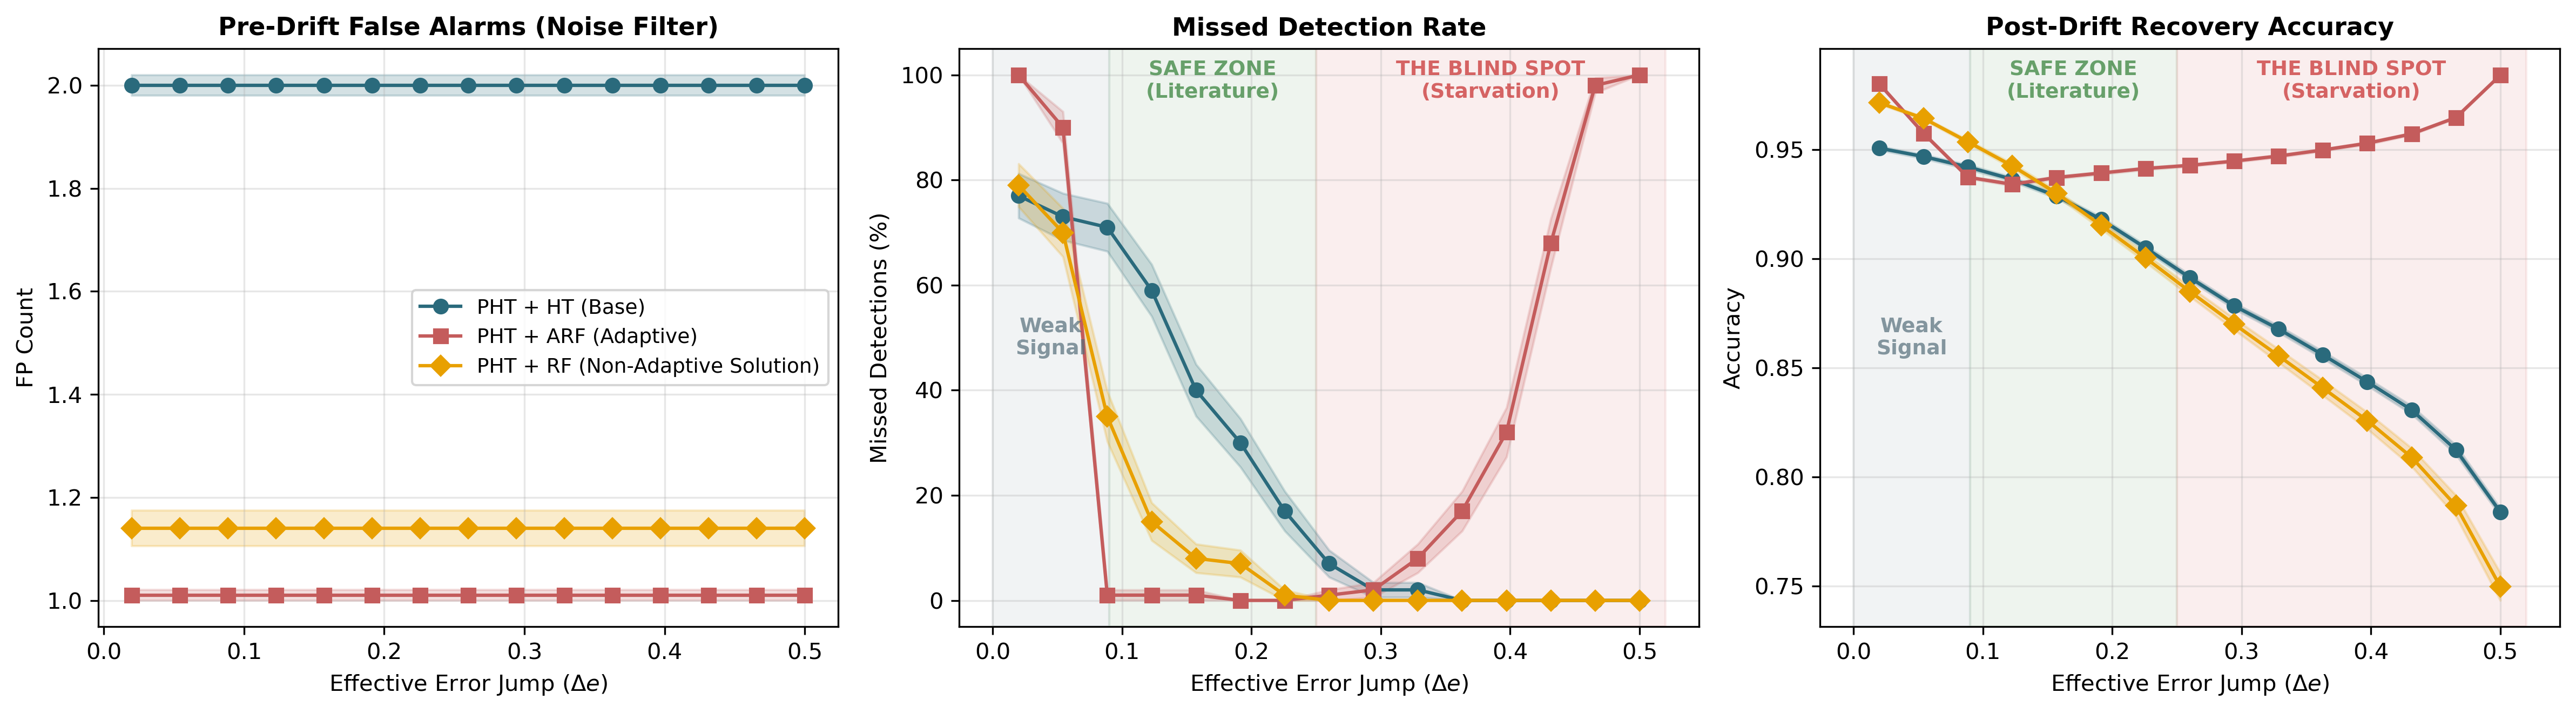
\includegraphics[width=0.90\textwidth]{Fig_R3_Regime_Crossover.png}
  \caption{The Regime Crossover and Architectural Resolution ($100$ streams/point, bands $=\pm 1$ SEM). \textbf{Left (Weak Signal):} models fail to trigger CUSUM. \textbf{Middle (Safe Zone, $\Delta e{\approx}0.15$):} ARF outperforms HT (literature consensus). \textbf{Right (Blind Spot, $\Delta e{\ge}0.25$):} the ARF's fast recovery starves the PHT (missed detections climb monotonically across the band, from $1\%$ at its first grid point $\Delta e{=}0.26$ to $100\%$ at $\Delta e{=}0.50$). A Non-Adaptive RF (yellow) inherits ARF's variance reduction (left) while keeping HT's persistent error signal (right), eradicating starvation (center).}
  \label{fig:crossover_and_solution}
\end{figure*}

As demonstrated in Figure~\ref{fig:crossover_and_solution}, deconstructing the metrics provides the physical mechanism behind the phenomenon and bridges our discovery with the literature consensus.

\textbf{1. The Weak Signal Zone ($\Delta e < 0.09$):} Models fail to accumulate sufficient signal within tolerance. The HT exhibits an artifactual miss rate reaching $77\%$ due to \emph{stochastic resonance}: its high variance generates random error bursts breaching the CUSUM threshold ($\lambda=25$). The ARF (red curve) suppresses this noise via Bagging variance reduction, avoiding early alarms.

\textbf{2. The Safe Zone ($\Delta e \in[0.09, 0.25]$):} In the magnitude zone typical of classic benchmarks, the ARF leverages \emph{background trees} to act as a powerful stochastic filter, perfectly stabilizing the CUSUM trajectory and halving pre-drift False Alarms compared to the HT (Fig.~\ref{fig:crossover_and_solution}, left).

\textbf{3. The Blind Spot Regime ($\Delta e \ge 0.25$):} Ensemble onset acceleration speeds up the ARF's post-drift recovery (Fig.~\ref{fig:crossover_and_solution}, right), and starvation follows (Fig.~\ref{fig:crossover_and_solution}, center): the evidence is erased before the external CUSUM accumulates it. The monitor is starved, driving missed detections to 100\% or producing delayed post-recovery alarms.

\noindent\textbf{On the absence of a closed-form crossover prediction.}
Classical first-passage bounds for transient CUSUM~\cite{tartakovsky_2023_transient,tartakovsky_2014} (Markov, Doob reflection, Siegmund ARL) predict a roughly \emph{uniform} missed-detection probability across $\Delta e \in [0.05, 0.50]$ under the canonical model ($\lambda{=}25$, $\delta_P{=}0.005$, $K_{\mathrm{ARF}}{\approx}18.5$, $\hat\alpha{\approx}0.98$), in contrast with the sharp transition of Fig.~\ref{fig:crossover_and_solution}. The empirical boundary thus does not reduce to canonical theory: it emerges from the joint dynamics of River's adaptive mean-tracking PHT~\cite{montiel_river_2021} (distinct from the fixed-$p_0$ model of Eq.~\eqref{eq:cusum}), the bimodal $\tau_{\mathrm{ARF}}$ in the Safe Zone, and noise swaps (Remark~\ref{rem:bgswap}). A derivation of $\Delta e_{\mathrm{crit}}$ jointly modelling these is left to future work.

The Blind Spot Phenomenon is thus not a contradiction of the literature, but its asymptotic extension.

\textbf{Validation on real-world data streams.}
To validate the regime crossover boundary beyond synthetic distributions, we evaluated the phenomenon on six real-world streams: the Bank Account Fraud (BAF) tabular benchmark~\cite{jesus_baf_2022} in its three temporal-split variants (Base, Variant I, Variant II), and three variants of the INSECTS benchmark~\cite{souza_insects_2020} (\emph{abrupt\_balanced}, \emph{gradual\_balanced}, \emph{incremental\_reoccurring\_balanced}). We compute F1 over 30 random seeds per variant, evaluating true detections via a bipartite Hopcroft-Karp matching protocol~\cite{hopcroft_karp_1973}. The effective error jump $\Delta e$ is estimated drift-by-drift via an adaptive window protocol $w_k = \min(5000, \min(\Delta t_{\mathrm{left}}, \Delta t_{\mathrm{right}})/3)$ to avoid the overlapping-window artefact that fixed-window estimators produce on closely-spaced engineered drifts.

\textbf{Empirical frontier calibration.}
The six streams populate the regime-crossover boundary of Section~\ref{sec:crossover} continuously (Table~\ref{tab:real_data_summary}); all INSECTS positions follow Souza et al.~\cite{souza_insects_2020}, Table~2. The three BAF variants sit at $\Delta e \approx 0$ (Weak Signal zone), where the blind spot is dormant and the HT/ARF F1 ratio is indistinguishable from unity. This reading is not an artefact of the estimator being measured on an adapting model: a reference tree forked at the end of the warm-up and never retrained reports the same $\Delta e \approx 0$ at the same canonical positions ($|\Delta e| < 0.001$, every interval covering zero). A frozen model cannot absorb a change, so a jump it does not see is not one adaptation has erased. Both trees in fact sit at the majority-class error rate, which on these streams is the fraud rate itself: no Hoeffding-tree pipeline acquires discriminative signal on BAF, so no error transient exists for any monitor to miss. BAF is therefore an explicit \emph{negative control} for the phenomenon, and the demonstration rests on the two high-magnitude INSECTS variants. INSECTS \emph{abrupt\_balanced} ($\Delta e \approx 0.07$) is a \emph{weak witness}: its five canonical jumps are heterogeneous and partly negative ($\Delta e \in \{0.68, -0.15, 0.24, -0.27, -0.13\}$) and both detectors fire near their false-alarm rate, so its marginal ARF advantage is not mechanistically attributable. The effect appears on the two high-magnitude variants, and through \emph{false-alarm flooding}, not starvation. On \emph{gradual\_balanced} ($\Delta e \approx 0.45$, single transition) PHT+HT detects genuinely ($7$ alarms, precision $0.14$, F1 $0.25$) whereas PHT+ARF($c{=}1$) sprays $86$ alarms (precision $0.012$, F1 $0.02$)---a $10.57\times$ F1 gap (sign test $p \le 2^{-29}$, the resolution floor of the two-sided test at $30$ seeds) driven entirely by precision; \emph{incremental\_reoccurring\_balanced} ($\Delta e \approx 0.39$) confirms the same mode more moderately ($1.61\times$, $p \le 2^{-29}$). We state this plainly: the predicted \emph{starvation} (recall $\to 0$) is observed only on the synthetic stationary streams (Bernoulli, ProteuS), while the real non-stationary streams exhibit its dual, \emph{flooding} (precision $\to 0$; Remark~\ref{rem:flooding}).\footnote{The evaluated set is the three balanced INSECTS variants with discrete change points held in the artifact repository. Table~2 of Souza et al.~\cite{souza_insects_2020} lists eleven streams, and the other eight are not evaluated: \emph{incremental\_balanced}, which has no discrete drift positions and so admits no tolerance matching, \emph{incremental\_abrupt\_balanced}, the five imbalanced variants, and \emph{out-of-control}. No $\Delta e$ is computed or reported for them.}

\begin{table*}[ht]
  \centering
  \caption{Real-world validation across six streams ($30$ seeds/cell). Drift positions follow Souza et al.~\cite{souza_insects_2020} Table~2 (`reoccurring\_balanced' retains $K{=}2$ in-stream transitions). F1 numerator is deterministic here; per-cell dispersion reflects classifier initialization. Significance: seed-level sign test, where $2 \cdot 10^{-9}$ is the resolution floor $2^{-29}$ of the two-sided test at $30$ seeds. $p_0$: the classifier's own mean error over the armed pre-change span, external detector disabled, median over seeds. The $c{=}1$ clock degrades monitoring via `false-alarm flooding' (precision collapse), not starvation: on `gradual\_balanced', PHT+ARF($c{=}1$) emits 86 alarms for one drift (precision $0.012$) vs 7 for PHT+HT ($0.14$). `abrupt\_balanced' is a weak witness (heterogeneous, partly negative jumps; neither beats false-alarm rate).}
  \label{tab:real_data_summary}
  \resizebox{\textwidth}{!}{\begin{tabular}{@{}lcccccccc@{}}
\toprule
Variant & $\Delta e$ & F1(PHT+HT) & F1(PHT+ARF$_{c=1}$) & F1(ADW+ARF$_{c=1}$) & Ratio HT/ARF & Sign test $p$ & $p_0$ HT & $p_0$ ARF$_{c=1}$ \\
\midrule
BAF Base & $\approx 0$ & $0.10$ & $0.10$ & $0.00$ & $1.00$ & --- & $0.012$ & $0.012$ \\
BAF Variant I & $\approx 0$ & $0.09$ & $0.11$ & $0.00$ & $0.83$ & --- & $0.011$ & $0.011$ \\
BAF Variant II & $\approx 0$ & $0.00$ & $0.00$ & $0.00$ & --- & --- & $0.011$ & $0.011$ \\
INSECTS abrupt\_balanced & $0.07$ & $0.13$ & $0.18$ & $0.48$ & $0.71$ & $4 \cdot 10^{-2}$ & $0.375$ & $0.262$ \\
INSECTS gradual\_balanced & $0.45$ & $0.25$ & $0.02$ & $0.06$ & $10.57$ & $2 \cdot 10^{-9}$ & $0.314$ & $0.164$ \\
INSECTS reoccurring\_balanced & $0.39$ & $0.31$ & $0.19$ & $0.16$ & $1.61$ & $2 \cdot 10^{-9}$ & $0.400$ & $0.232$ \\
\bottomrule
\end{tabular}
}
\end{table*}

\subsection{A Constructive Solution: The Non-Adaptive Ensemble}\label{sec:solution_rf}

The evaluation in Section~\ref{sec:crossover} shows that bagging itself does not starve the monitor: a static forest does not. Nor is tree-swapping the root cause of the erasure: within the adaptive forest, counterfactual arms that share one stream and fork at $\tau^*$ assign $\LearnSharePure\%$ of it to incremental learning with no tree replaced, $\SwapFirstShare\%$ to the first replacement and $\SwapRestShare\%$ to all later ones (Remark~\ref{rem:first_swap}). A \emph{Non-Adaptive Random Forest} (RF)---a static bagging of Hoeffding Trees operating without internal ADWINs---is the architecture that removes the starvation regime on the streams tested, wherever a cumulative-evidence monitor would otherwise lose the transient.

As demonstrated by the yellow curves in Figure~\ref{fig:crossover_and_solution}, deploying an RF fully resolves the phenomenon by decoupling variance reduction from adaptation. In the pre-drift phase (Fig.~\ref{fig:crossover_and_solution}, left), the RF provides the identical noise-filtering capability as the ARF, significantly reducing false alarms compared to the unstable HT baseline. In the post-drift phase (Fig.~\ref{fig:crossover_and_solution}, right), the RF's accuracy degrades in parallel with the HT, ensuring that the error signal remains persistent rather than transient. Consequently, the external PHT operates exactly as mathematically intended, removing starvation and maintaining a flawless $0\%$ missed detection rate even under massive structural shifts ($\Delta e = 0.50$, Fig.~\ref{fig:crossover_and_solution}, center).

To validate this architectural resolution under extreme realistic conditions, we evaluated both PHT and ADWIN monitors coupled with the static RF against the heteroscedastic ProteuS streams of Section~\ref{sec:proteus}; these rows now occupy the final block of Table~\ref{tab:results_concept}, generated under the same aligned method as the baselines. The empirical result is definitive \emph{for cumulative-evidence monitors}: while the default PHT + ARF systematically fails to detect any drift (F1 = 0.00) due to starvation, substituting the ARF with a static RF restores the pipeline. The PHT + RF achieves robust F1-scores from $0.73 \pm 0.05$ (IID Baseline) to $0.96 \pm 0.02$ (Cal. B)---the headline $0\%$ missed-detection figure above is a \emph{recall} statement, while this F1 ceiling is precision-limited by tolerance-window matching, not by any missed drift. A seed-level sign test confirms complete separation against the starved PHT + ARF ($913/1080$ vs $0/1080$ runs detected, all $30$ seeds favouring the RF, $p \le 2^{-29}$). The fix is therefore \emph{specific to the starvation regime}, not universal: for the windowed ADWIN monitor---not starved at $c = 1$ on these streams (Section~\ref{sec:proteus})---the adaptive ARF detects marginally \emph{more} than the static RF ($1070/1080$ vs $959/1080$; all $30$ seeds favouring the ARF, $p \le 2^{-29}$). The RF is thus the resolution where a cumulative monitor would otherwise starve, not a universal replacement for adaptation.

Furthermore, the Non-Adaptive RF keeps a stable Average Detection Delay across all GARCH regimes ($\mathrm{ADD} \approx 19$--$20$ for PHT, $\approx 12$--$14$ for ADWIN), confirming that static ensembles yield an uncontaminated error stream insensitive to the input heteroscedasticity.

This monitoring fidelity comes at a measurable predictive cost: as visible in Fig.~\ref{fig:crossover_and_solution} (right), the static RF's post-drift accuracy decays alongside HT and falls below ARF by up to $23.4$ percentage points at $\Delta e = 0.50$ (RF $\approx 0.750$ vs ARF $\approx 0.984$). The trade-off is therefore architectural rather than incidental: practitioners must size the ensemble for monitoring fidelity rather than predictive optimality. We treat this as a deliberate design choice and discuss extensions coupling static ensembles with dynamic CUSUM thresholds in Section~\ref{sec:limitations}.

% ══════════════════════════════════════════════════════════════════
\section{Discussion}\label{sec:discussion}

\begin{table*}[t]
  \centering
  \small
  \caption{Monitor families on the error stream at their deployed and equalised false-alarm
  levels, indexed by the pre-change error rate $p_0$ of the stream. Detection inside the
  exploitable transient and the pre-change alarm rate are means over $20$ magnitudes of $100$
  runs on the raw error stream; the delay is the median over magnitudes of the per-magnitude
  median. The equalised levels place ADWIN and KSWIN at the requirement of a CUSUM at
  $\lambda = 15$, derived with $\tau_{\mathrm{swap}}^{(1/M)} = 57.4$ in place of $W$; at the
  exploitable transient itself no ADWIN level in $(0, 1]$ matches that requirement. At $p_0 = 0$
  the null is degenerate and no false-alarm level is defined; only EDDM's arming state is reported
  there. EDDM carries its arming rate and median arming instant beside its delay.}
  \label{tab:family_order}
  \resizebox{\textwidth}{!}{%
  \begin{tabular}{llrlrrr}
    \toprule
    family & setting & $p_0$ & armed & pre-change alarms & detected in $W$ & median delay \\
    \midrule
    EDDM & published & $0.000$ & never, $0/1080$ & --- & $0.000$ & --- \\
    \midrule
    StrictCUSUM, $\lambda = 15$ & published & $0.024$ & --- & $0.000$ & $0.928$ & $35.0$ \\
    StrictCUSUM, $\lambda = 50$ & published & $0.024$ & --- & $0.000$ & $0.001$ & $1089.0$ \\
    PHT, $\lambda = 15$ & published & $0.024$ & --- & $0.000$ & $0.928$ & $33.5$ \\
    PHT, $\lambda = 50$ & published & $0.024$ & --- & $0.000$ & $0.000$ & --- \\
    ADWIN & published & $0.024$ & --- & $0.000$ & $0.885$ & $28.0$ \\
    ADWIN & equalised & $0.024$ & --- & $0.000$ & $0.926$ & $15.0$ \\
    KSWIN & published & $0.024$ & --- & $0.000$ & $0.458$ & $27.0$ \\
    KSWIN & equalised & $0.024$ & --- & $0.000$ & $0.337$ & $28.0$ \\
    EDDM & published & $0.024$ & $1.000$ at $t_{\mathrm{rel}} = +16$ & $0.020$ & $0.974$ & $17.5$ \\
    \midrule
    StrictCUSUM, $\lambda = 15$ & published & $0.069$ & --- & $0.000$ & $0.958$ & $31.5$ \\
    StrictCUSUM, $\lambda = 50$ & published & $0.069$ & --- & $0.000$ & $0.448$ & $440.0$ \\
    PHT, $\lambda = 15$ & published & $0.069$ & --- & $0.030$ & $0.942$ & $28.0$ \\
    PHT, $\lambda = 50$ & published & $0.069$ & --- & $0.000$ & $0.090$ & $391.0$ \\
    ADWIN & published & $0.069$ & --- & $0.000$ & $0.891$ & $32.0$ \\
    ADWIN & equalised & $0.069$ & --- & $0.000$ & $0.933$ & $18.5$ \\
    KSWIN & published & $0.069$ & --- & $0.000$ & $0.572$ & $27.2$ \\
    KSWIN & equalised & $0.069$ & --- & $0.000$ & $0.478$ & $28.8$ \\
    EDDM & published & $0.069$ & $1.000$ at $t_{\mathrm{rel}} = -554$ & $0.930$ & $0.022$ & $40.0$ \\
    \bottomrule
  \end{tabular}}
\end{table*}
% ══════════════════════════════════════════════════════════════════

\subsection{Practical Implications}
Default configurations (e.g., River's ARF at $c_{\mathrm{int}} = 1$) mask strong drifts from a cumulative monitor. Reliable monitoring is obtained with either a non-adaptive classifier, or an external clock faster than the internal one ($c_{\mathrm{ext}} < c_{\mathrm{int}}$); neither is necessary (Definition~\ref{def:decoupling}).

\begin{figure*}[t]
  \centering
  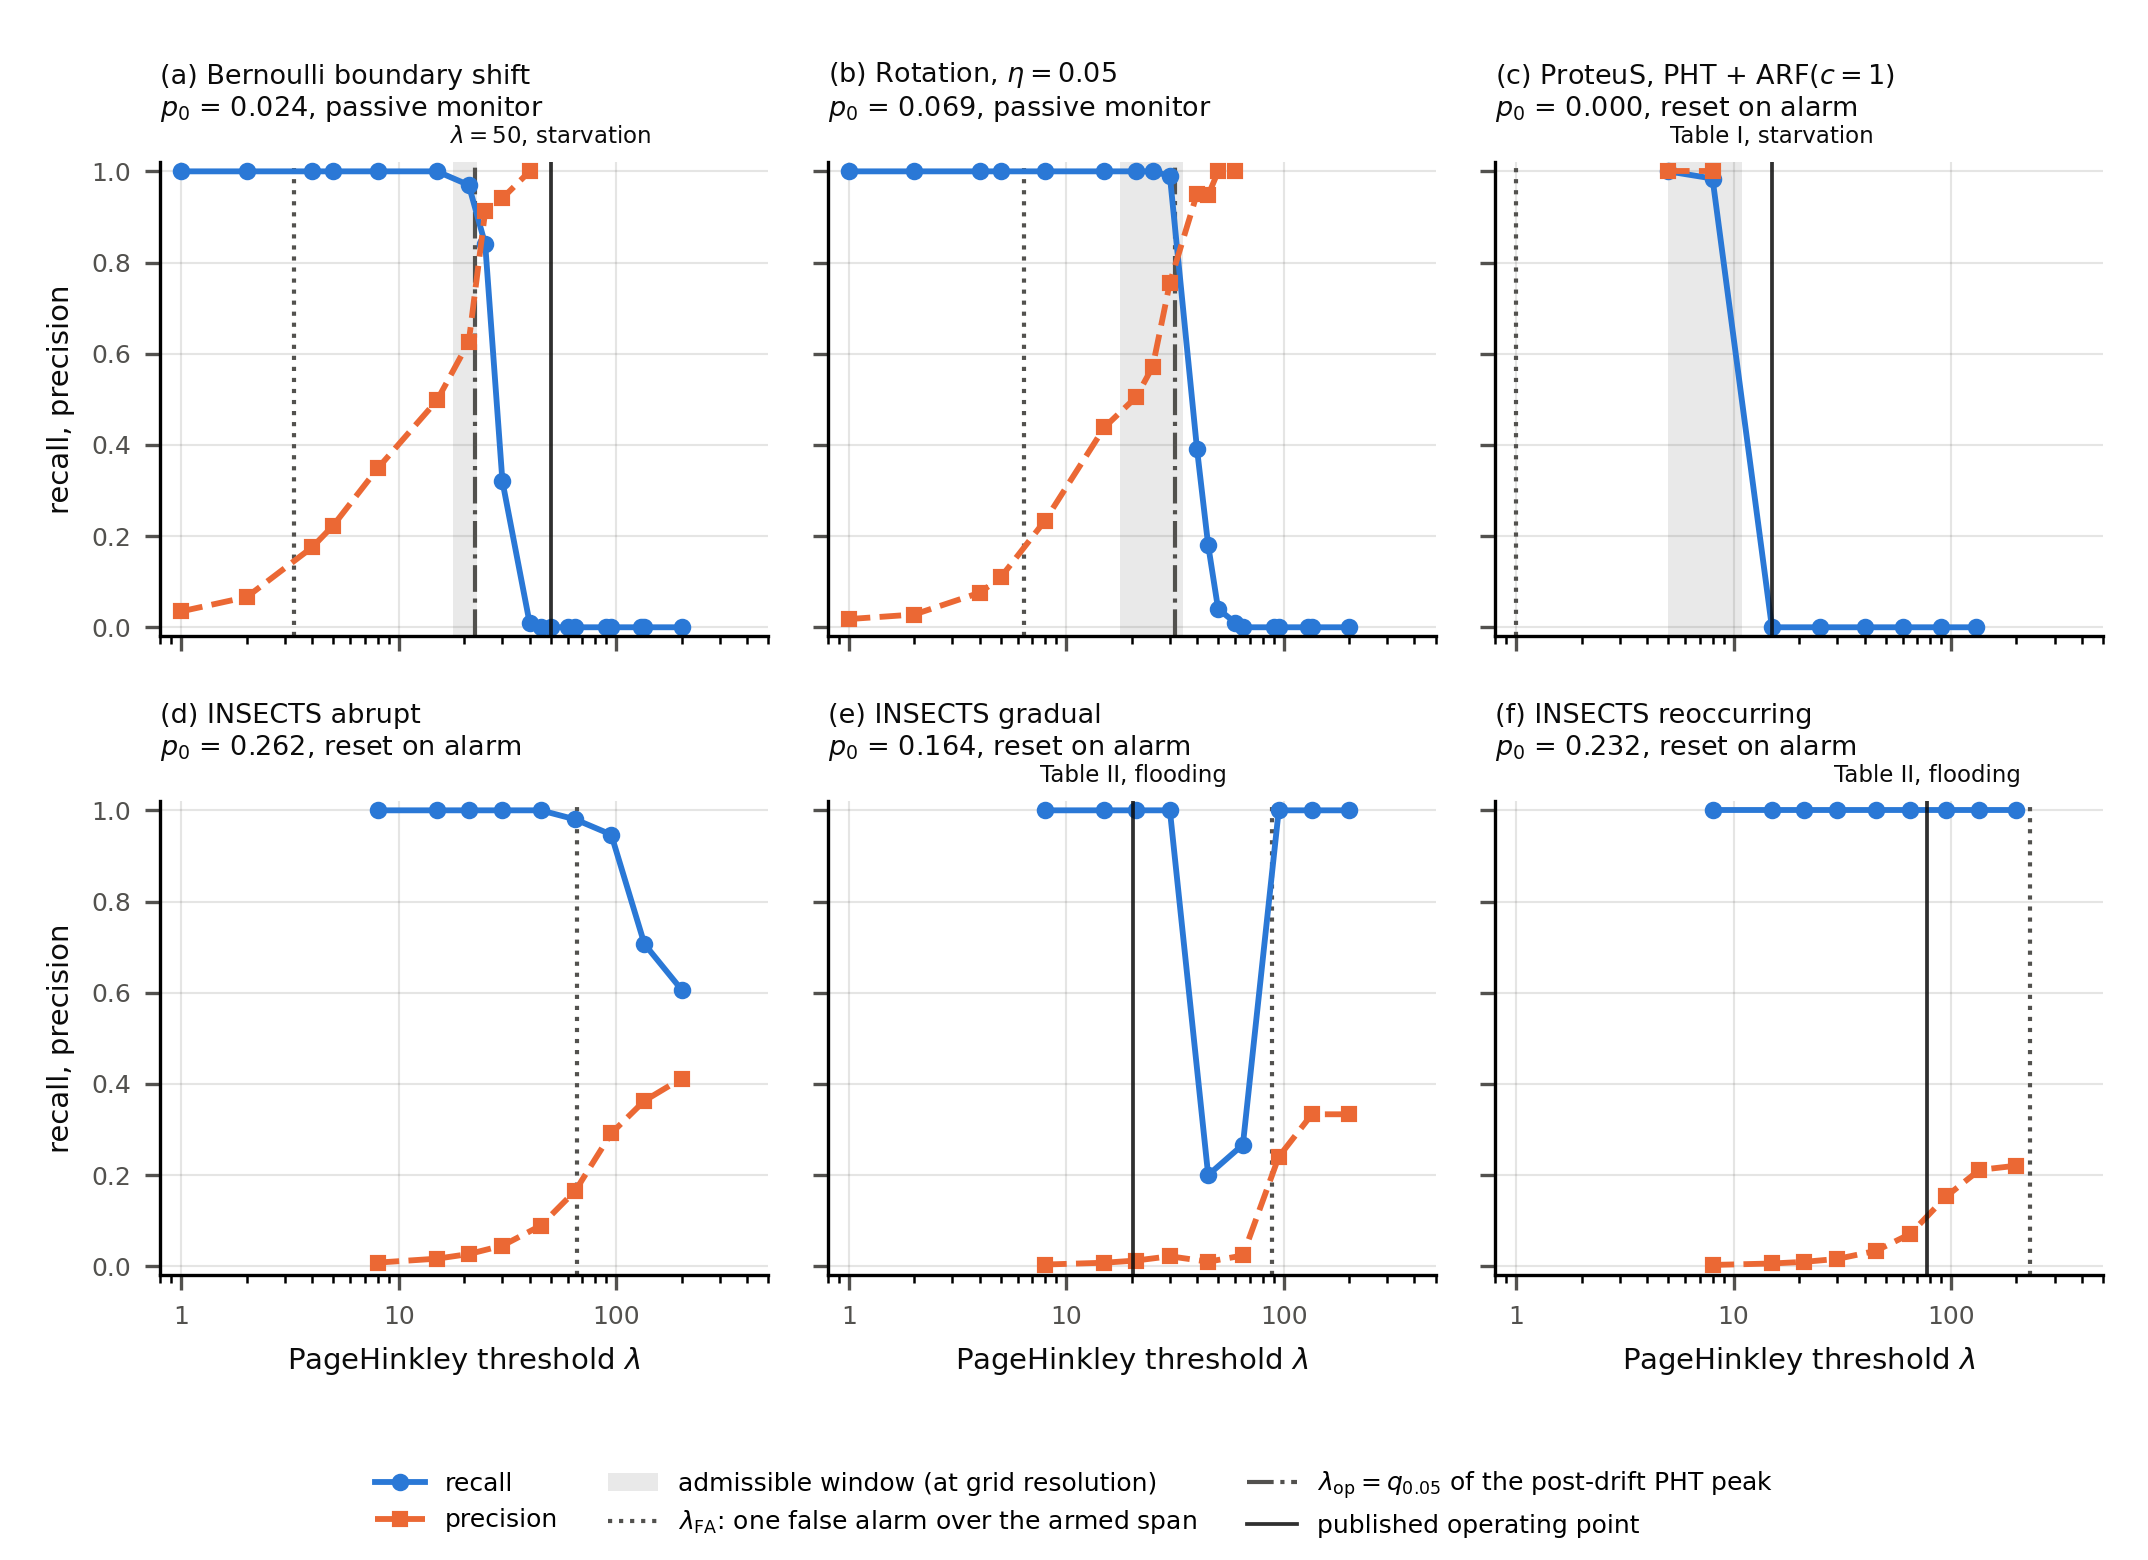
\includegraphics[width=\textwidth]{figures/Fig_S10_dual_mode.png}
  \caption{Starvation and flooding on one axis. Recall (solid) and precision (dashed) against the
    PageHinkley threshold on six streams; shaded: thresholds with recall $\ge 0.95$ and precision
    $\ge 0.5$, at the grid's resolution. Dotted: the threshold buying one false alarm over the armed
    pre-change span; dash-dot: the $5\%$ quantile of the post-drift statistic peak. (a,~b)~canonical
    and rotation families at $\Delta e = 0.327$, passive monitor; (c)~ProteuS; (d--f)~INSECTS,
    monitor and classifier reset on each alarm. Every published failure fails by one criterion:
    starvation by recall, flooding by precision. No threshold is admissible on INSECTS with the ARF
    at $c = 1$.}
  \label{fig:dual_mode}
\end{figure*}

\textbf{The Fundamental Tension.} Figure~\ref{fig:dual_mode} places starvation and flooding on one threshold axis. The tension is an envelope property, not a universal one. Instrumented on the canonical grid at $\delta_P = \DeltaPtext$, the measured evidence ceiling gives $q_{0.05}(S_{\max}) = \QlowFloorLo$ at $\Delta e = \DeFloorLo$ and $\QlowFloorHi$ at $\Delta e = \DeFloorHi$. The admissible set $\{\lambda \ge \LambdaFA\} \cap \{\lambda \le \lambda_{\mathrm{op}}\}$ is therefore empty for every envelope floored at or below $\DeFloorLo$, and non-empty for every envelope floored at or above $\DeFloorHi$; the boundary lies strictly inside that interval, measured at $\Delta e_c = \DeCrit$ ($95\%$ bootstrap CI $\DeCritCI$, $n=300$). Restricting the envelope to $[\EnvLo, \EnvHi]$, where the post-change class prior stays at $10\%$, leaves the admissible set non-empty. The infeasibility claim of the submitted version held only because the envelope reached below the detectability floor. This forces a choice among three architectural fixes:
\textbf{(S1) Detector-side:} Window-divergence monitors (e.g., KSWIN) do not accumulate evidence and are far less sensitive to a short transient; on the settings we test they restore detection at no predictive cost.
\textbf{(S2) Classifier-side:} A Static Random Forest ($\tau_{\mathrm{ARF}} = \infty$) removes the CUSUM tension at a $23.4$ percentage-point post-drift accuracy cost, isolating internal adaptation as the driver.
\textbf{(S3) Macro-architecture:} A two-tier protocol in which the external monitor commands the ensemble swap keeps S1's monitoring fidelity together with S2's long-term recovery.

\subsection{Limitations and Future Work}\label{sec:limitations}
\textbf{Limitations.} First, tracking internal swaps aggregates true detections with continuous background noise, preventing isolated ARL$_0$ comparisons. Second, evaluating adaptive pipelines on the canonical (ARL$_0$, ADD) plane confounds noise filtering with detection survival; resolving against the control threshold $\lambda$ is required to isolate the collapse. Third, the starvation boundary is stated distribution-free, and its tighter conditional form needs a conditional independence the shared generator does not deliver (Appendix~\ref{sec:dep_gate}); the shortfall of the measured acceleration ($4$--$8\times$) from the $M$-fold reference ($10\times$ at $M{=}10$) is carried mostly by the non-exponential delay law, not by inter-tree correlation (Section~\ref{sec:hydra}). Fourth, the ProteuS pre-drift error is identically zero on every run of both arms, so the false-alarm side of Table~\ref{tab:results_concept} is void: no threshold on those streams is bought at a false-alarm cost, the $\alpha$ sweep of KSWIN cannot move a false-alarm rate, and $\lambda = \LambdaFA$ is an operating threshold rather than a calibration. Finally, the phenomenon is regime-dependent: standard benchmarks (SEA, Hyperplane) operate at low magnitudes ($\Delta e \lesssim 0.15$), masking the starvation condition and shielding standard pipelines from the blind spot.

\textbf{Label latency.} The external monitor reads an error stream, and every error waits for its label. We measured delays of $l \in \{10, 50, 100, 500\}$ steps on the canonical and rotation families ($100$ seeds $\times$ $20$ magnitudes). The outcome depends on who waits. If only the monitor waits, erasure stays where it was and the alarm moves by $l$: detection before erasure at $\lambda = 15$ falls from $0.92$ to $0.24$ at $l = 500$ on the canonical family, with the evidence itself unchanged. If the classifier learns from the same delayed labels, adaptation recedes with them: the erasure instant moves by $0.998\,l$ at $l = 500$, the evidence read before it grows $2.5$-fold, and the starvation threshold $\lambda = 50$ detects $90\%$ of drifts instead of $5\%$. Latency penalises a monitor through the delay it adds \emph{beyond} the classifier's; a shared latency trades detection delay for a longer, larger transient.

\textbf{Future Work.} Three directions emerge. \emph{First}, extending Empirical Result~\ref{res:budget_sufficient}, which already covers Streaming Random Patches and leveraging bagging~\cite{bifet_leveraging_2010}, beyond its nine pipelines and six magnitudes. \emph{Second}, formalizing the externalized two-tier architecture (S3) or exploring windowed-detector pairings (e.g., ADWIN+ARF) that retain the ensemble's variance-reduction benefits without starvation. \emph{Third}, developing a closed-form derivation of the transition threshold ($\lambda^* \approx 15$--$25$) from the joint $\tau_{\mathrm{ARF}}$/CUSUM dynamics.

% ══════════════════════════════════════════════════════════════════
\section{Conclusion}\label{sec:conclusion}
% ══════════════════════════════════════════════════════════════════

We formalized the \textbf{blind spot} as a deficit of the evidence an adaptation leaves against the evidence a monitor's calibration requires, both in one unit (Definition~\ref{def:blindspot}). On the instrumented forests the roles separate: the internal ADWIN fixes the onset of adaptation; incremental learning with no tree replaced performs $\LearnSharePure\%$ of the erasure; and the first replacement carries more of the remainder than all later ones together ($\SwapFirstShare\%$ against $\SwapRestShare\%$) and sets the thresholded decision, with $\AbInitDetect$ detections in $100$ when replacement is suppressed from $\tau^*$ against $\NoSwapLeak$ when it is suppressed only after the first. Ensemble onset acceleration moves the onset earlier; it does not drive the erasure. No critical ensemble size is certifiable from the distribution-free envelope (Corollary~\ref{cor:mcrit}), and the race is measured instead. Windowed and distributional monitors are not exempt: read at the false-alarm level of a $\lambda = 50$ CUSUM, their requirements exceed the measured evidence ceiling as well (Remark~\ref{rem:split_measured}).

The reactivity condition of Definition~\ref{def:decoupling} is sufficient, not necessary. Below the detectability floor, bounding false alarms on heteroscedastic streams requires a threshold above the evidence ceiling and the admissible calibration set is empty; above it a calibration exists. The operational rule is to set the threshold from the false-alarm budget of the span the monitor will run armed over, on the error stream of the classifier it will be paired with, and to check that the resulting requirement lies below the measured ceiling. A distribution-based monitor such as KSWIN detects on ProteuS, whose pre-drift error is identically zero, at no predictive cost; on the instrumented Bernoulli family it is the weakest of the five monitors measured at equal false-alarm cost.

\appendix
% docs/manuscript/sections/prop3_v2.tex
% Appendix: the domain of Proposition 3, W as a random variable,
% and the proofs of thm:floor (tightened), prop:invariance and cor:split.
% Every numeral is read from results/S2_theory/tables/ or results/S6_synchronized_traces/tables/.
% Produced by experiments/S2_theory/{s2_arl0.py, s2_w_random.py, s2_eddm.py}.

\section{The Starvation Bound: Domain, Randomness of \texorpdfstring{$W$}{W}, and Proofs}\label{sec:prop3}

\subsection{Where Eq.~\eqref{eq:markov_bound} says anything}\label{sec:prop3_domain}

Proposition~\ref{prop:starvation} is sound: Azuma--Hoeffding applied to the
centred walk, Doob's maximal inequality on the exponential submartingale, a
union bound over the at most $W$ reflection restart points, with the
$\sqrt{W \ln(W/\varepsilon)}$ fluctuation margin retained and $s_0$ carried
explicitly. What was never stated is the set on which it is not vacuous.

\begin{definition}[Informative domain]\label{def:eq4_domain}
  Eq.~\eqref{eq:markov_bound} bounds a probability, so its content is
  $\min\{1,\, W e^{-\frac{2}{W}(\lambda - s_0 - \mu W)_+^2}\}$. Write
  \[
    \mathcal{D} \;:=\; \bigl\{ (W, \lambda) \;:\; \mu W < \lambda - s_0 \bigr\},
    \qquad \mu := \Delta e - \delta_P .
  \]
  Outside $\mathcal{D}$ the positive part vanishes, the exponential is $1$, and
  the bound returns $W \ge 1$: it is \emph{vacant}. Membership of $\mathcal{D}$
  is necessary but not sufficient --- $W e^{-\frac{2}{W}(\cdot)^2}$ must also
  fall below $1$ --- and the two criteria are reported separately below.
\end{definition}

Instantiated at $\delta_P = \DeltaPtext$, $s_0 = 0$, on the measured
estimators of $W$ (mean over $100$ seeds per magnitude, arm \texttt{full},
the argmax read on the charged walk at the declared tolerance) and
the threshold ladder $\lambda \in \{8, 15, 25, 50\}$, the $240$ pairs split
$188$ vacant and $52$ inside $\mathcal{D}$, of which $32$ yield a bound
strictly below $1$. At the canonical magnitude $\Delta e = 0.3268$:

\smallskip
\centerline{\begin{tabular}{lrrrrr}
  \toprule
  $W$ estimator & mean $W$ & $\mu W$ & $\lambda = 15$ & $\lambda = 25$ & $\lambda = 50$ \\
  \midrule
  $\tau_{\mathrm{swap}}^{(1/M)}$ & 57.4  & 18.2  & vacant & $1.0$ & $2.7\!\times\!10^{-14}$ \\
  $W_{\mathrm{argmax}}$          & 390.6 & 123.8 & vacant & vacant & vacant \\
  $\tau_{\mathrm{err}}(0.10)$    & 557.0 & 176.4 & vacant & vacant & vacant \\
  \bottomrule
\end{tabular}}
\smallskip

\noindent This is Remark~\ref{rem:transient_length} verified rather than
asserted: $\mu W = \SixMuWfirst$ at the first replacement and $\SixMuWerase$ at
erasure reproduce from the recomputation at the declared tolerance to the
printed precision ($W_{\mathrm{argmax}}$ is the argmax of the
$\delta_P = 0.01$ walk; the $611.9$ of the superseded $\delta_P = 0.005$ walk
is retired with it). The remark's
diagnosis is also correct and is the one that matters --- the hypothesis that
fails is the \emph{constant accumulation rate} $\mu$ across the window, not the
fluctuation term. The error excess decays inside the window; a bound that
charges it at rate $\mu$ for the whole of $W$ is bounding a trajectory that does
not occur.

Two readings deserve to be separated. Across the grid, Eq.~\eqref{eq:markov_bound}
is informative essentially only at $\lambda = 50$ under the first-swap window,
and at $\lambda = 25$ for $\Delta e \ge 0.436$. That is a narrow domain --- and
it contains the operating point at which the starvation certificate is stated.
The proposition is not vacuous where it is used; it is vacuous almost everywhere else.

\subsection{\texorpdfstring{$W$}{W} is a random variable}\label{sec:prop3_random}

Treating a random window as a constant is not admissible here.
Proposition~\ref{prop:starvation} is stated at a single $W$, and the campaign
measures a distribution whose spread straddles $\partial\mathcal{D}$. The
statement that bounds the ensemble of runs is therefore

\begin{equation}\label{eq:eq4_integrated}
  \mathbb{P}(S^* \ge \lambda)
  \;\le\;
  \mathbb{E}_W\Bigl[\min\bigl\{1,\, W e^{-\frac{2}{W}(\lambda - s_0 - \mu W)_+^2}\bigr\}\Bigr],
\end{equation}
the expectation taken over the law of $W$ at that magnitude, by conditioning on
$W$ and applying Eq.~\eqref{eq:markov_bound} pathwise.

\begin{remark}[The cap is not cosmetic, and it fixes a floor]\label{rem:eq4_cap}
  A run whose transient exceeds the horizon contributes $T_h = \SixHorizon$ to
  the uncapped integrand, so an uncapped ``bound'' reports $2500$ on a
  probability. Capped, such a run contributes exactly $1$, and
  \eqref{eq:eq4_integrated} is bounded below by the censoring fraction alone:
  $\mathbb{E}_W[\cdot] \ge \mathbb{P}(W \ge T_h)$ at every $\lambda$. On the
  arm integrated over, that fraction is $8.21\%$ ($162$ of $1{,}974$
  complete-case runs; $8.20\%$, $164$ of $2{,}000$, on the whole arm). Any
  claim that \eqref{eq:eq4_integrated} is small at some $\lambda$ is therefore
  bounded away from truth by the censoring before the drift magnitude is even
  consulted.
\end{remark}

Two estimators bracket the integral. The plug-in holds censored runs at their
censoring time and so understates $W$ and the bound; the parametric estimator
integrates the log-normal accelerated-failure-time law already fitted to these
traces with exact right censoring, and so extrapolates past the horizon. Over
the twenty magnitudes:

\smallskip
\centerline{\begin{tabular}{rccc}
  \toprule
  $\lambda$ & deterministic $\bar{W}$ & plug-in & parametric \\
  \midrule
   8 & $1.000$ & $1.000$ & $0.9994$--$1.000$ \\
  15 & $1.000$ & $1.000$ & $0.9902$--$1.000$ \\
  25 & $1.000$ & $1.000$ & $0.9487$--$0.9998$ \\
  50 & $1.000$ & $1.000$ & $0.7526$--$0.9951$ \\
  \bottomrule
\end{tabular}}
\smallskip

\noindent Treating $W$ as random does not repair Eq.~\eqref{eq:markov_bound};
it makes its vacancy unconditional. The deterministic and plug-in readings are
vacant at every magnitude and every threshold. The parametric reading is
formally non-vacant, and its best value over the whole grid is $0.753$: a bound
of $0.75$ on a crossing probability whose measured value is $0.000$ at
$\lambda = 50$. We report that as what it is --- the bound is not wrong, it is
empty --- and we do not present it as a repair.

\subsection{What actually carries the published result}\label{sec:prop3_loadbearing}

Proposition~\ref{prop:certificate} is deterministic. Its chain
$S_{\max}(H) \ge A_{\mathrm{swap}} \ge A_{\mathrm{sig}}(H) - H\delta_P$ uses no
distributional assumption, no rate model and no window length; it is an
inequality between three quantities measured on the same trajectory. Both
Definition~\ref{def:decoupling}(i-bis) and Empirical
Result~\ref{res:tension} route through $A_{\mathrm{swap}}$, and the
synchronised campaign states outright that $W^*$ is the wrong sufficient
statistic: at $\Delta e = 0.3268$, $\kappa$ exceeds its critical value by a
factor of $6$ to $18$ on $100\%$ of runs --- the gate that was supposed to
falsify the $\lambda = 50$ certificate --- and the certificate nonetheless holds,
with $0$ detections in $100$ runs, because the ceiling
$S_{\max} = 31.3$ (the reflected peak at the declared tolerance,
Remark~\ref{rem:split_measured}) is simply below $\lambda = 50$ however long
the transient lasts.

Proposition~\ref{prop:certificate} is therefore the load-bearing statement.
Proposition~\ref{prop:starvation} is a scope statement: it says where a
fluctuation argument can still say something about the crossing probability,
and \S\ref{sec:prop3_domain} says that this is a small set. The two are not in
competition and neither subsumes the other.

\paragraph{The removal branch, argued on both sides.}
Keeping Eq.~\eqref{eq:markov_bound} costs a proposition that is vacant at the
measured operating point under two of its three window estimators, and invites
a referee to ask why a bound that returns $\ge 1$ on $188$ of $240$ measured
configurations is in the paper at all. Removing it costs the only statement
that quantifies the fluctuation margin --- the $\sqrt{W \ln(W/\varepsilon)}$
term, which is what explains why the empirical crossover is a finite-width
stochastic transition rather than a sharp threshold --- and the only bridge to
the post-transient reading of Remark~\ref{rem:sufficient}.

The rule fixed before the domain table was computed retains it on a
non-empty informative domain and withdraws it on an empty one. The domain is
not empty: $32$ of $240$ measured pairs, including the $(\lambda = 50,
W = \tau_{\mathrm{swap}}^{(1/M)})$ pair at which the certificate is stated.
Eq.~\eqref{eq:markov_bound} is therefore \textbf{retained, restricted to
$\mathcal{D}$, and demoted}: it is presented as a scope statement about
fluctuation arguments, with its domain table, and never as the mechanism of the
blind spot. The mechanism is Proposition~\ref{prop:certificate}.

\subsection{Proofs}\label{sec:prop3_proofs}

\begin{proof}[Proof of Theorem~\ref{thm:floor}, and its tightening]
  The proof in \S\ref{sec:requirement} is complete as there stated, under the
  two hypotheses the theorem now names, and is not restated. Two points are
  recorded.

  \emph{The chain rule.} $\mathrm{KL}(P_1 \Vert P_0) = \sum_t \mathbb{E}_1
  \bigl[d(\pi_t \Vert \pi_t^{(0)})\bigr]$ holds for the laws of
  the $W$ observed errors in the conditional form, the expectation being over
  the filtration generated by the past. The product-of-marginals expression
  $\sum_t d(\bar{e}_t \Vert p_0)$ is a \emph{lower} bound on this sum ---
  $d$ is convex in its first argument, so
  $\mathbb{E}_1[d(\pi_t \Vert p_0)] \ge d(\mathbb{E}_1[\pi_t] \Vert p_0)$ ---
  and is never used as an upper bound. What the chord and $\chi^2$ steps
  need is that $\pi_t - p_0$ be confined to $[0, \Delta_{\max}]$ almost
  surely and that the conditional null rate be $p_0$ after every past, and
  those are hypotheses~(ii) and~(i), now stated on the theorem and measured
  at the operating point in \S\ref{sec:requirement}: the upper end of~(ii)
  at $\Delta_{\max} = 0.36$ (the frozen-at-$\tau^*$ arm), the lower end
  measured false only in the adapted tail past the transient. The earlier
  reading --- $\Delta_{\max}$ as a maximum of \emph{unconditional}
  expectations, $0.3268$ --- substituted a different constant and is retired
  with it.

  \emph{The relaxation.} The step $d(x \Vert y) \le (x-y)^2/(y(1-y))$ is the
  $\chi^2$ bound, applied $W$ times. It is unnecessary: $u \mapsto
  d(p_0 + u \Vert p_0)$ is convex on $[0, \Delta_{\max}]$ and vanishes at
  $u = 0$, so the chord through the endpoints gives
  $d(p_0+u \Vert p_0) \le (u/\Delta_{\max})\,d_{\max}$ with $d_{\max} :=
  d(p_0 + \Delta_{\max} \Vert p_0)$, whence $\mathrm{KL}(P_1 \Vert P_0) \le
  (d_{\max}/\Delta_{\max})(A + W\delta_P)$ and Eq.~\eqref{eq:floor_chord}.
  Since $d_{\max} \le \Delta_{\max}^2/(p_0(1-p_0))$ is the same $\chi^2$ bound
  applied once, \eqref{eq:floor_chord} is never weaker
  than~\eqref{eq:floor}. At $p_0 = 0.024$, $\Delta_{\max} = 0.36$ the ratio
  is $7.08$; over the sensitivity band $[0.015, 0.032]$ it runs from $9.51$ to
  $5.98$. The relaxation is loosest exactly where the measured base rate sits,
  which is why it was invisible at the assumed $p_0 = 0.05$.
  \textbf{Status: PROVED} (as stated, under its named hypotheses), and
  tightened.
\end{proof}

\begin{proof}[Proof of Proposition~\ref{prop:invariance}]
  Under hypothesis~(i), $A = (\Delta e - \delta_P)W$; substituting
  hypothesis~(ii), $W = K(\Delta e)^{-\alpha}$, gives
  $A = K(\Delta e)^{-\alpha}(\Delta e - \delta_P) =
  K(\Delta e)^{1-\alpha}(1 - \delta_P/\Delta e)$, which is
  Eq.~\eqref{eq:invariance}. At $\alpha = 1$ the prefactor is $1$ and
  $A = K(1 - \delta_P/\Delta e) \to K$ as $\Delta e/\delta_P \to \infty$,
  monotonically from below. \textbf{Status: PROVED UNDER STATED CONDITION.}

  The condition is the whole content of the caveat. Hypothesis~(i) is the
  rectangular surrogate, withdrawn on measurement: $A/A_{\mathrm{rect}}$ spans
  $2.70$ to $-14.12$ and changes sign. Hypothesis~(ii) holds at
  $\hat\alpha \approx 0.98$, and Eq.~\eqref{eq:invariance} then predicts a
  spread of $(\Delta e)^{0.02}$, a factor $1.03$ over
  $\Delta e \in [0.10, 0.50]$, against a measured factor of $1.76$ that is not
  monotone. The proposition is thus a true statement about a model the measurements contradict, and it explains $3\%$ of a $90\%$ effect. What
  survives is Remark~\ref{rem:invariance_measured}'s counterfactual: the same
  ceiling on the branch where adaptation is suppressed spreads by a factor of
  $133$ and is monotone.
\end{proof}

\begin{proof}[Proof of Corollary~\ref{cor:split}]
  Fix $W$, $\varepsilon$, $n_{\mathrm{stat}}$ and let $\alpha \to 0$. The
  $\varepsilon$-margin $\sqrt{(W/2)\ln(1/\varepsilon)}$ is common to the three
  and constant, so only the $\alpha$-price matters.

  \emph{CUSUM.} $\lambda(\alpha)$ is defined by
  $\alpha = W/\mathrm{ARL}_0(\lambda)$ with Siegmund's
  $\mathrm{ARL}_0(\lambda) = (e^{\theta^* \lambda} - \theta^*\lambda - 1)/
  (\theta^*\delta_P)$. Taking logarithms,
  $\theta^*\lambda = \ln(1/\alpha) + \ln(W\theta^*\delta_P) + \ln(1 +
  O(\theta^*\lambda e^{-\theta^*\lambda}))$, so
  $\lambda(\alpha) = \theta^{*-1}\ln(1/\alpha)\,(1+o(1))$: linear in
  $\ln(1/\alpha)$, with no $W$ in the leading term.

  \emph{ADWIN and KSWIN.} By Eqs.~\eqref{eq:Radwin}--\eqref{eq:Rkswin} the
  $\alpha$-prices are $\sqrt{(W/2)\ln(4W/\alpha)}$ and
  $\sqrt{n_{\mathrm{stat}}\ln(2/\alpha)}$, both
  $\Theta(\sqrt{\ln(1/\alpha)})$ at fixed $W$ and $n_{\mathrm{stat}}$.

  A linear function of $\ln(1/\alpha)$ exceeds any square-root function of it
  beyond a finite crossing point, so for every fixed budget $A$ there is
  $\alpha^\dagger > 0$ below which $R_{\mathrm{CUSUM}} > A \ge
  R_{\mathrm{ADWIN}} \wedge R_{\mathrm{KSWIN}}$ fails for the cumulative monitor
  alone. The $W$-scalings are read directly off the same three expressions:
  $\lambda(\alpha)$ carries no $W$; $\sqrt{(W/2)\ln(4W/\alpha)} \to 0$ as
  $W \to 0$ because $W\ln W \to 0$; and $\sqrt{n_{\mathrm{stat}}\ln(2/\alpha)}$
  carries no $W$ either. \textbf{Status: PROVED.}

  The last of those three corrects the submitted statement, which placed the
  $\alpha$-price of $R_{\mathrm{KSWIN}}$ ``inside a square root of $W$''.
  Eq.~\eqref{eq:Rkswin} contains no such $W$, and the correction matters: KSWIN
  escapes not because its requirement vanishes with the transient but because
  its $\alpha$-price is set by the statistic size, which the practitioner
  chooses, instead of by a threshold that must grow like $\ln(1/\alpha)$.
  Remark~\ref{rem:split_measured} evaluates all three at a common $\alpha$ and
  exhibits the crossing at $\ln(1/\alpha) = 16.34$ against the windowed two-sample 
  monitor and $18.97$ against the adaptive-window monitor.
\end{proof}

\subsection{EDDM}\label{sec:prop3_eddm}

No $R_{\mathrm{EDDM}}$ is delivered, and the requirement is withdrawn from the
family of \S\ref{sec:requirement}.

EDDM compares $p'_i + 2s'_i$, the cumulative mean and standard deviation of
inter-error distances since the last reset, against the running maximum of that
same path. Modelling the distances as geometric at rate $p_0$ before the change
and $p_1$ after, and writing $f$ for the post-change share of errors since the
reset, $d := 1/p$ and $\sigma^2 := (1-p)/p^2$,
\begin{equation}\label{eq:eddm_level}
  \mathrm{level}(f) =
  \frac{(1-f)d_0 + f d_1 + 2\sqrt{(1-f)\sigma_0^2 + f\sigma_1^2
        + f(1-f)(d_0-d_1)^2}}{d_0 + 2\sigma_0},
\end{equation}
decreasing from $\mathrm{level}(0) = 1$, so detection requires
$f \ge f^\dagger := \inf\{f : \mathrm{level}(f) < \beta\}$ and hence
$W_{\mathrm{EDDM}} = (n_0/p_1)\,f^\dagger/(1-f^\dagger)$ post-change steps,
with $n_0$ the pre-change error count since the last reset. The between-group
term $f(1-f)(d_0-d_1)^2$, which the normal approximation on geometric distances
omits, grows with the contrast at the same time as the mean falls, and the two
largely cancel: $f^\dagger$ is nearly invariant in the drift magnitude, $0.235$
to $0.240$ over $p_1 \in [0.10, 0.70]$, so $W_{\mathrm{EDDM}} \approx
0.31\, n_0/p_1$. It therefore shortens with the drift magnitude much as a
first-passage time does. What distinguishes it is the factor $n_0$: a threshold
test requires an \emph{absolute} amount of evidence, whereas EDDM requires a
fixed \emph{share} of its own history, so its requirement grows without bound as
the stationary phase lengthens. No first-passage bound carries such a term.

This closed form does not reproduce the measured collapse, and the rule fixed in
advance makes withdrawal the outcome in that case. At the ProteuS pre-change
history it returns $168$--$281$ steps against the normal approximation's $155$:
the same order of magnitude, not the ``no detection'' that $0$ alarms in
$1{,}080$ runs requires. Worse, it cannot be evaluated where the collapse is
measured: the ProteuS artifacts record $F_1$, ADD and seed and no error stream,
so neither $p_0$ nor $p_1$ nor the transient length is available there.

The one stream on which the inputs do exist cannot arbitrate either. On the
synchronised traces, the detector has not completed its $30$-error warm start at
the change point in $95\%$ of runs --- $1{,}000$ pre-change steps at
$p_0 = 0.024$ furnish about $24$ errors --- so every alarm is post-warm-start by
construction; on the \texttt{static} arm, which does warm up, it alarms
\emph{before} the change point in $60\%$ of runs. The decisive control is that
the three adaptive arms return the same alarm rate to within $0.08$, although
they differ by exactly the adaptation under study, and the \texttt{frozen} arm
never adapts at all. A statistic that cannot tell those three apart is not
reporting on drift.

The \emph{empirical} EDDM result is independent of this: $0$ detections in $1{,}080$ runs against $882$ for the same detector on a non-adaptive learner, sign test $p \approx 1.9\times10^{-9}$, is a measurement and stands on its own. What is not established is that a requirement $R_{\mathrm{EDDM}}$ of the form of Eqs.~\eqref{eq:Rcusum}--\eqref{eq:Rkswin} governs it.

\subsection{Proof status}\label{sec:prop3_status}

\centerline{\begin{tabular}{llp{0.42\linewidth}}
  \toprule
  Statement & Status & Condition \\
  \midrule
  Thm.~\ref{thm:floor} & PROVED & hypotheses (i)--(ii) stated and measured;
    tightened by Eq.~\eqref{eq:floor_chord} \\
  Prop.~\ref{prop:invariance} & PROVED UNDER STATED CONDITION &
    rectangular transient and $\alpha = 1$; both measured false \\
  Cor.~\ref{cor:split} & PROVED & at fixed $W$, $\varepsilon$,
    $n_{\mathrm{stat}}$, as $\alpha \to 0$ \\
  Prop.~\ref{prop:order} & PROVED & drift not resolved before the first
    replacement; holds on $1{,}835/1{,}836$ estimable runs \\
  $R_{\mathrm{EDDM}}$ & NOT PRODUCED & withdrawn; the empirical result stands \\
  \bottomrule
\end{tabular}}

% docs/manuscript/sections/dependence_v2.tex
% Stream S3, deliverable 1. Replaces the v63 material of sec:starvation_boundary: the equality of
% Eq. (eq:pmiss), the independence assumption behind it, the Correlation disclaimer, cor:mcrit and
% the numerical example. Also carries the resolution of the F22 contradiction, which belongs to
% sec:hydra and is referenced from there rather than patched into it.
% Every numeral is read from results/S3/. Produced by
% experiments/S3_dependence/{s3_gate_rng_factorization.py, s3_bounds.py, s3_competing_risks.py}.

\section{Inter-Tree Dependence and the Starvation Boundary}\label{sec:dependence}

The submitted version of Proposition~\ref{prop:starvation_boundary} asserted an \emph{equality}
for $P_{\mathrm{miss}}$ under a conditional independence of the per-tree delays that was never
demonstrated, against a \emph{deterministic} accumulation time $\tau_{\mathrm{det}}^*$. The main text
states the repaired proposition; this appendix derives its three components: the equality replaced
by a two-sided distribution-free envelope, the independence assumption by a named and measured
hypothesis, and $\tau_{\mathrm{det}}^*$ by the competing-risks formulation of
Section~\ref{sec:dep_race}.

\subsection{What the bound needs, and what positive correlation gives}\label{sec:dep_correlation}

The \emph{Correlation disclaimer} argued that because the $M$ trees are trained on the same stream
through Poisson-weighted bagging~\cite{gomes_arf_2017}, the delays $\tau_i$ are positively
correlated, and that the independence formula therefore \emph{overestimates} $P_{\mathrm{miss}}$.
The conclusion is right; the stated reason is not sufficient for it.

\begin{remark}[Positive correlation does not imply the bound]\label{rem:corr_insufficient}
  Writing $A_i := \{\tau_i \le s\}$, the inequality
  $\mathbb{P}(\min_i \tau_i \le s) \le 1 - [1 - F(s)]^M$ requires positive \emph{association of the
  indicators at the level $s$}, i.e.\ $\mathbb{P}(A_i \cap A_j) \ge F(s)^2$. Pearson correlation of
  the delays does not deliver that at every level. Take $M = 2$ and the exchangeable law placing
  mass $0.3$ on each of $(1, 100)$ and $(100, 1)$, $0.2$ on $(2,2)$ and $0.2$ on $(200,200)$. At
  $s = 2$: $F(2) = 0.5$, $\mathbb{P}(A_1 \cap A_2) = 0.20 < 0.25 = F(2)^2$, hence
  $\mathbb{P}(\min \le 2) = 0.80 > 0.75 = 1 - [1 - F(2)]^2$ --- the bound is violated --- while
  $\mathrm{Corr}(\tau_1, \tau_2) = +0.51$.
\end{remark}

What rescues the inequality here is not correlation but the \emph{common-factor} structure: the $M$
trees see one data stream, and conditioning on it is exactly the hypothesis of
Proposition~\ref{prop:min_jensen}. The disclaimer is restated on that mechanism below and is no
longer an assertion about a sign.

\subsection{Two bounds on the minimum}\label{sec:dep_bounds}

Throughout, $\tau_{\mathrm{ARF}} = \min_{1\le i\le M} \tau_i$ by Eq.~\eqref{eq:hydra}, $F$ is the
marginal CDF of one tree \emph{inside} the ARF, $s$ is a deterministic level, and $\mathcal{S}$
denotes the $\sigma$-field of the common data stream.

\begin{proposition}[Exchangeability bound]\label{prop:min_jensen}
  If $(\tau_1, \ldots, \tau_M)$ are exchangeable and conditionally independent given
  $\mathcal{S}$, then for every $s$
  \begin{equation}\label{eq:jensen_bound}
    \mathbb{P}\!\left(\min_i \tau_i \le s\right) \;\le\; 1 - \bigl[1 - F(s)\bigr]^M .
  \end{equation}
\end{proposition}

\begin{proof}
  Let $G_{\mathcal{S}}(s) := \mathbb{P}(\tau_i > s \mid \mathcal{S})$, which does not depend on $i$
  by exchangeability. Conditional independence gives
  $\mathbb{P}(\min_i \tau_i > s \mid \mathcal{S}) = G_{\mathcal{S}}(s)^M$. The map $x \mapsto x^M$
  is convex on $[0,1]$, so by Jensen's inequality and the tower property,
  \[
    \mathbb{P}\!\left(\min_i \tau_i > s\right) = \mathbb{E}\bigl[G_{\mathcal{S}}(s)^M\bigr]
      \;\ge\; \bigl(\mathbb{E}[G_{\mathcal{S}}(s)]\bigr)^M = \bigl[1 - F(s)\bigr]^M ,
  \]
  and Eq.~\eqref{eq:jensen_bound} follows by complementation.
\end{proof}

\begin{corollary}[Direction of the disclaimer]\label{cor:disclaimer}
  Under the hypothesis of Proposition~\ref{prop:min_jensen}, the independence formula is an
  \emph{upper} bound on $P_{\mathrm{miss}}$, not an approximation of unknown sign. This is the
  content the \emph{Correlation disclaimer} asserted, now derived; by
  Remark~\ref{rem:corr_insufficient} it does not follow from positive correlation alone.
\end{corollary}

\begin{proposition}[Distribution-free envelope]\label{prop:min_boole}
  For every $s$ and \emph{any} dependence structure whatever,
  \begin{equation}\label{eq:boole_bound}
    F(s) \;\le\; \mathbb{P}\!\left(\min_i \tau_i \le s\right) \;\le\; \min\bigl(1,\, M F(s)\bigr).
  \end{equation}
  Both ends are attained, so the envelope cannot be tightened without a dependence hypothesis.
\end{proposition}

\begin{proof}
  $\{\min_i \tau_i \le s\} = \bigcup_i A_i$ with $A_i := \{\tau_i \le s\}$. Sub-additivity gives
  $\mathbb{P}(\bigcup_i A_i) \le \sum_i \mathbb{P}(A_i) = M F(s)$, and a probability is at most
  $1$; monotonicity gives $\mathbb{P}(\bigcup_i A_i) \ge \mathbb{P}(A_1) = F(s)$. Attainment is the
  Fr\'echet--Hoeffding pair for a union of $M$ equiprobable events.
\end{proof}

\subsection{The shared generator does not factorise}\label{sec:dep_gate}

Whether Eq.~\eqref{eq:jensen_bound} may be used is a question about River's implementation, not
about the model. Instrumenting the forest generator on one trajectory
($M = 10$, $c_{\mathrm{int}} = 1$, $300$ warm-up and $200$ probe steps) gives a verdict.

\begin{remark}[Draw-stream factorisation, measured]\label{rem:rng_gate}
  River threads a single \texttt{random.Random} through the whole forest~\cite{montiel_river_2021}:
  \texttt{model.data[i].rng is model.\_rng} holds on all ten trees. Sharing the object is not
  decisive; the factorisation of the draw stream is. Two channels consume it. The Oza weight is a
  rejection loop costing $k+1$ uniforms for a returned weight $k$, so its cost is itself random;
  and with two features and \texttt{max\_features}$\,=\,$\texttt{'sqrt'} the feature subsample draws
  at every leaf creation, an event fixed by the drawing tree's own state. Measured: the draws
  consumed per (step, tree) range over $1$--$16$ with mean $7.07$, so no tree owns the deterministic
  residue class $\{i, M{+}i, 2M{+}i, \ldots\}$; and perturbing the state of one tree displaces
  $9839$ of the positions consumed by the others, the first at position $34$. The ensemble vote does
  not enter per-tree learning (\texttt{ARFClassifier.\_drift\_detector\_input} is
  $\mathbf{1}[\hat{y}_i \ne y]$ on the member's own prediction), so the trees are coupled through
  the generator or not at all.
\end{remark}

We therefore do \emph{not} use Eq.~\eqref{eq:jensen_bound} for any published quantity. It is stated
with its hypothesis named, and the claim is carried by the distribution-free
Eq.~\eqref{eq:boole_bound}. The criterion is conservative rather than sharp: a displacement of
positions proves state-dependence of the allocation, whereas a sequential allocation by adapted
stopping times would preserve independence on an idealised i.i.d.\ source. We record that gap
explicitly, and note that conditional independence given $\mathcal{S}$ is not a measurable property
of a deterministic generator at all --- conditioned on stream and seed, every delay is a constant.

\subsection{The single-tree plug-in is refuted by the measurement}\label{sec:dep_plugin}

Both bounds are statements about $F$, the marginal of a tree \emph{inside} the ARF. No artifact in
this work records it: Proposition~\ref{prop:starvation_boundary} substituted $\widehat{F}$, the
empirical CDF of the standalone HAT delays $\tau_{\mathrm{HAT}}$ at $M = 1$. That substitution is
testable at $M = 10$, because the instrumented ARF campaign measures
$\mathbb{P}(\tau_{\mathrm{ARF}} \le s)$ directly on the same seeds and magnitudes.

\begin{empresult}[The HAT marginal is not the member marginal]\label{res:plugin_refuted}
  Over the $80$ testable cells ($20$ magnitudes $\times$ $\lambda \in \{8, 15, 25, 50\}$, $M = 10$,
  $n = 100$ runs each), the plug-in bound $\min(1, M\widehat{F}(s))$ falls strictly below the Wilson
  $95\%$ lower end of the measured proportion in \textbf{$10$ cells} ($11$ for
  Eq.~\eqref{eq:jensen_bound}), all at $\lambda \le 25$. The mechanism is the left tail: at
  $\Delta e = \SixCanonDeltaE$ the fastest of $100$ HAT runs adapts at step $33$, so
  $\widehat{F}(25.25) = 0$ exactly, while $4$ of $100$ ARF runs have already adapted by that step.
  Symmetrically, the slowest member is up to twice as slow as $\widehat{F}$ predicts:
  $\mathbb{E}[\tau_{(10)}]$ measured against $\mathbb{E}[\max$ of $10$ draws from $\widehat{F}]$
  gives a ratio falling from $1.09$ at $\Delta e = 0.028$ to $0.49$ at $\Delta e = 0.498$.
\end{empresult}

The refutation is of the \emph{substitution}, not of either inequality:
Eq.~\eqref{eq:boole_bound} holds unconditionally for the true $F$. What the measurement establishes
is that the ARF member's delay law is \emph{more dispersed} than the HAT's at both tails, which is
what Poisson weighting and a one-feature split rule would produce. No numeral of
Eq.~\eqref{eq:pmiss} is therefore published through $\widehat{F}$, and the numerical example of the
v63 section is retracted rather than recomputed.

\subsection{Critical ensemble size, withdrawn}\label{sec:dep_mcrit}

\begin{remark}[Why $M_{\mathrm{crit}}$ does not survive]\label{rem:mcrit_withdrawn}
  Corollary~\ref{cor:mcrit} inverts Eq.~\eqref{eq:pmiss} in $M$. That inversion exists only for the
  exchangeability form: the distribution-free envelope \emph{saturates} as soon as $M F(s) \ge 1$,
  and in the saturated region $\min(1, M F(s))$ does not depend on $M$ at all. At $M = 10$
  saturation begins at $F \ge 0.10$, which is everywhere this work operates
  ($\widehat{F} = 0.28$ at $\lambda = 25$ and $0.49$ at $\lambda = 50$, both at
  $\Delta e = \SixCanonDeltaE$, saturating from $M = 4$ and $M = 3$ respectively). With
  Eq.~\eqref{eq:jensen_bound} unavailable by Remark~\ref{rem:rng_gate} and $\widehat{F}$ refuted by
  Empirical Result~\ref{res:plugin_refuted}, $M_{\mathrm{crit}}$ has neither a bound to invert nor a
  CDF to invert it on. It is withdrawn, and replaced by the measured incidence of
  Section~\ref{sec:dep_race}.
\end{remark}

What the proposition retains is the envelope of Eq.~\eqref{eq:boole_bound} stated on $F$, with the
equality of Eq.~\eqref{eq:pmiss} replaced by an inequality. That is strictly weaker than the v63
statement and is published as such. We note for completeness that the alternative --- withdrawing
the proposition entirely --- was considered: $\mathrm{Prop.}$~\ref{prop:certificate} is
deterministic, carries no distributional hypothesis, and already routes the published result
through $A_{\mathrm{swap}}$ (Definition~\ref{def:decoupling}, Empirical
Result~\ref{res:tension}). The envelope is retained because it remains informative
($\le 0.5$) at $132$ of the $384$ operating points of the grid $\Delta e \ge 0.24$,
$\lambda \in \{8, 15, 25, 50\}$, $M \ge 2$, and because it is the only statement that ties ensemble
size to miss probability without a distributional assumption.

\subsection{The race is a competing risk, not a threshold comparison}\label{sec:dep_race}

$\tau_{\mathrm{det}}$ is a stopping time. Replacing it by the scalar
$\tau_{\mathrm{det}}^* = \lambda/(\Delta e - \delta_P)$ discards its dispersion and its censoring,
and makes the race monotone in $\Delta e$ by construction. We estimate instead the cumulative
incidence of the two causes under a single administrative censoring at the common horizon
$t_c = 4000$ post-drift steps.

\begin{empresult}[Measured incidence of the race]\label{res:cif}
  On the instrumented campaign ($20$ magnitudes $\times$ $\SixSeeds$ seeds, paired-on-seed
  percentile bootstrap, $10{,}000$ replicates), the race carries \emph{no censored unit}:
  $\tau_{\mathrm{ARF}}$ is observed on every run at every magnitude, so a monitor that never crosses
  $\lambda$ has \emph{lost} the race rather than gone unobserved. At $\lambda = 50$ the monitor
  wins $0.0000$ of the $2{,}000$ runs --- $\mathbb{P}(\tau_{\mathrm{ARF}} < \tau_{\mathrm{det}}) = 1$
  with bootstrap band $[1.00, 1.00]$ at every magnitude --- and the five alarms it does raise
  ($0.25\%$) all fire after the ensemble has adapted. At $\lambda = 25$ the monitor wins $0.042$ on
  average, and \emph{non-monotonically}: $0.00$ at $\Delta e = 0.028$, a maximum of $0.32$ at
  $\Delta e = 0.141$, then $0.00$ from $\Delta e = 0.361$ upward. At $\lambda = \LambdaFA$ the
  measured miss probability at $M = 10$ rises from $0.26$ to $0.62$ across the grid.
\end{empresult}

The hump at $\lambda = 25$ is the starvation effect stated as a probability: a weak drift does not
move the error stream enough to cross $\lambda$ inside the window, and a strong one is erased before
the accumulation completes. It is invisible through $\tau_{\mathrm{det}}^*$, which is monotone in
$\Delta e$ by construction --- which is the substantive reason for removing the scalar, beyond its
being the wrong object.

\subsection{Effective ensemble size}\label{sec:dep_meff}

No artifact records the per-tree $\tau_i$; the instrumented campaign records four order statistics
per run, $\tau_{\mathrm{swap}}^{(q)}$ for $q \in \{0.10, 0.25, 0.50, 1.00\}$, i.e.\ $\tau_{(1)}$,
$\tau_{(3)}$, $\tau_{(5)}$, $\tau_{(10)}$ at $M = 10$. The residual dependence is therefore
bracketed, never point-estimated.

\begin{empresult}[Two bracketing estimates, reported as an interval]\label{res:meff}
  Method of moments under exchangeability, using the four order statistics through a trapezoidal
  quantile $L$-estimator of the run mean (calibrated at $+4.8\%$ on independent synthetic draws),
  returns $\widehat{\rho} \in [-0.021, 0.053]$ and $M_{\mathrm{eff}} \in [6.79, 12.28]$ across the grid.
  Direct order-statistic matching against $\widehat{F}$, which never passes through $\rho$, returns
  $M_{\mathrm{eff}}$ falling monotonically from $11.3$ to $5.1$. The two agree within a declared
  factor of $1.5$ at $13$ of $20$ magnitudes and \emph{disagree} at the remaining seven; both are
  reported and neither is averaged into the other. At $\Delta e = \SixCanonDeltaE$ the interval is
  $M_{\mathrm{eff}} \in [6.99, 9.16]$ against a nominal $M = 10$.
\end{empresult}

The disagreement is structured rather than noisy, and Empirical
Result~\ref{res:plugin_refuted} explains it: the direct route absorbs the marginal mismatch into
$M_{\mathrm{eff}}$, the moment route does not. \textbf{The measured within-run correlation of the
swap times is not distinguishable from zero.}

\subsection{The exponential reference, and what the shortfall is made of}\label{sec:dep_exponential}

\begin{remark}[Reading the multichart null]\label{rem:exponential_reference}
  The identity $\mathbb{E}[\tau_{(1:M)}] = \mathbb{E}[\tau_1]/M$ is a property of the exponential
  family, invoked in Section~\ref{sec:hydra} as a calibration reference. It is not a claim that the
  measured $\tau_{\mathrm{HAT}}$ is exponential, and it is not: a Lilliefors-style bootstrap
  Kolmogorov--Smirnov test ($N = 2000$ replicates, rate refitted on each) rejects exponentiality at
  \emph{all twenty} magnitudes, largest $p = 0.0030$. The two statements are consistent; they were
  written so that the first could be read as a property of the ARF, which it is not.
\end{remark}

Read as a quantitative null, the parallel-chart analogy~\cite{tartakovsky_2005_multichart} predicts
$10\times$ at $M = 10$, and Section~\ref{sec:hydra} attributes the measured shortfall to positive
inter-tree correlation. That attribution does not survive measurement. Evaluating the order
statistics of $\widehat{F}$ alone --- which would return exactly $M$ were $\widehat{F}$ exponential
--- gives an acceleration of $9.22\times$ at $\Delta e = \SixCanonDeltaE$ and $4.83\times$ at
$\Delta e = 0.141$, against measured factors of $7.99\times$ and $4.12\times$. The residual left for
dependence \emph{and} for the marginal mismatch of Empirical Result~\ref{res:plugin_refuted}
together is a factor of $0.87$ and $0.85$ respectively. \textbf{Non-exponentiality of the delay law,
not inter-tree correlation, accounts for most of the departure from $M$-fold}, and at
$\Delta e = 0.141$ for nearly all of it --- consistently with the near-zero $\widehat{\rho}$ of
Empirical Result~\ref{res:meff}. The decomposition is itself conditional on the refuted plug-in and
is reported as a bracket, never as a point attribution.

\subsection{Status of the v63 statements}\label{sec:dep_status}

\begin{center}\begin{tabular}{lll}
  \toprule
  object & v63 form & disposition \\
  \midrule
  \emph{Correlation disclaimer} & asserted sign & Cor.~\ref{cor:disclaimer}, proved; reason corrected \\
  Eq.~\eqref{eq:pmiss} & equality & Eq.~\eqref{eq:boole_bound}, two-sided envelope \\
  independence assumption & tacit & Prop.~\ref{prop:min_jensen}, named and \emph{measured to fail} \\
  $\tau_{\mathrm{det}}^*$ & deterministic scalar & removed; Emp.~Res.~\ref{res:cif} \\
  $\widehat{F}$ as member marginal & tacit & Emp.~Res.~\ref{res:plugin_refuted}, \emph{refuted} \\
  Cor.~\ref{cor:mcrit} & live corollary & \textbf{withdrawn} (Rem.~\ref{rem:mcrit_withdrawn}) \\
  numerical example & $M_{\mathrm{crit}} = 0$ at $r = 0.95$ & retracted with the plug-in \\
  $M$-fold exactness & read as a result & Rem.~\ref{rem:exponential_reference}, a reference \\
  \bottomrule
\end{tabular}\end{center}

Two quantities remain unmeasured and are named rather than estimated: the member marginal $F$
itself, and the false-alarm-budget-equalised form of the Hydra factor, which would require
recording the per-step pre-drift error stream of a single tree standalone and inside the ensemble.
Neither is approximated here.


% ──────────────────────────────────────────────────────────────────
\bibliographystyle{spmpsci}
\bibliography{IEEEabrv,articleA_biblio_v64}

\end{document}
